%%%%%%%%%%%%%%%%%%%%%%%%%%%%%%%%%%%%%%%%%%%%%%%%%%%%%%%%%%%%%%%%%%%%%%%  
%%% Short-Term Forecasting in SIR Systems:  
%%% Last edited by Ravi (June 9, 2015).  
%%%%%%%%%%%%%%%%%%%%%%%%%%%%%%%%%%%%%%%%%%%%%%%%%%%%%%%%%%%%%%%%%%%%%%%%  
  
\documentclass[11pt]{article} 
%\usepackage{latex8}  
\usepackage{times}  
%\usepackage{epsfig}  
%\usepackage{psfig}  
\usepackage{amsfonts}  
\usepackage{latexsym}  
\usepackage{amsmath}  
\usepackage[latin1]{inputenc}  
\usepackage{varioref}  
\usepackage{cite}  
  
\usepackage{fancybox}  
%% \usepackage{shadow}  
\usepackage{times}  
\usepackage{amsmath}  
\usepackage{amsfonts}  
\usepackage{latexsym}  
\usepackage{color}  
\usepackage{graphicx}  
\usepackage{subfig}  
\usepackage{lscape}  
\usepackage{url}

\usepackage{epigraph}  
%%\usepackage{patchcmd}  

%%\usepackage{framed}  

  
\setlength{\textheight}{9 in}  
\setlength{\textwidth}{6.3 in}  
\setlength{\oddsidemargin}{-0.0125 in}  
\setlength{\evensidemargin}{-0.0125 in}  
\setlength{\topmargin}{-0.5 in}  
\setlength{\parskip}{2pt}  

\setlength{\itemsep}{1pt}  

%% For use with the epigraph package

\setlength\epigraphwidth{10cm}
\setlength\epigraphrule{0pt}

%%\makeatletter
%%\patchcommand{\epigraph}{\@epitext{#1}}{\itshape\@epitext{#1}}{}{}
%%\makeatother
   
  
\newtheorem{theorem}{Theorem}[section]  
\newtheorem{lemma}[theorem]{Lemma}  
\newtheorem{corollary}[theorem]{Corollary}  
\newtheorem{fact}[theorem]{Fact}  
\newtheorem{claim}[theorem]{Claim}  
\newtheorem{observation}[theorem]{Observation}  
\newtheorem{definition}[theorem]{Definition}  
\newtheorem{proposition}[theorem]{Proposition}  
\newtheorem{example}[theorem]{Example}  
  
\newcommand{\calb}{\mbox{${\cal B}$}}  
\newcommand{\calc}{\mbox{${\cal C}$}}  
\newcommand{\calcp}{\mbox{${\cal C}'$}}  

\newcommand{\calco}{\mbox{$\mathcal{C}_1$}}
\newcommand{\calct}{\mbox{$\mathcal{C}_2$}}
\newcommand{\calcop}{\mbox{$\mathcal{C}_1'$}}
\newcommand{\calcodp}{\mbox{$\mathcal{C}_1''$}}

\newcommand{\calcdp}{\mbox{${\cal C}''$}}  
\newcommand{\calf}{\mbox{${\cal F}$}}  
\newcommand{\cale}{\mbox{${\cal E}$}}  
\newcommand{\cali}{\mbox{${\cal I}$}}  
\newcommand{\calp}{\mbox{${\cal P}$}}  
\newcommand{\cals}{\mbox{${\cal S}$}}  
\newcommand{\calt}{\mbox{${\cal T}$}}  
  
\newcommand{\calh}{\mbox{${\cal H}$}}  
\newcommand{\calr}{\mbox{${\cal R}$}}  
\newcommand{\cald}{\mbox{${\cal D}$}}  


\newcommand{\cnp}{\mbox{\textbf{NP}}}
\newcommand{\cnump}{\mbox{\textbf{\#P}}}

\newcommand{\ttrue}{\textsc{True}}
\newcommand{\tfalse}{\textsc{False}}
  
%% \newcommand{\reach}{{\textsc{Reachability}}}
%% \newcommand{\treach}{{$t$-\textsc{Reachability}}}

% box for end of proof  
\newcommand{\QED}{\hfill\rule{2mm}{2mm}\medskip}   

%% Additional newcommands from Anil.

\newcommand{\opt}{\text{OPT}}
\newcommand{\eopt}{E_{\text{OPT}}}
\newcommand{\prob}{\textsc{Spectral Radius Minimization}}
\newcommand{\expect}{\mathrm{Exp}}
\DeclareMathOperator*{\nodes}{nodes}
\DeclareMathOperator*{\walks}{walks}
\DeclareMathOperator*{\ct}{count}
  
  

\begin{document} 
%% !TEX root = ./gdsc-report.tex

\begin{titlepage}

{




%\center{\textcolor{red}{For Evaluation By PKDD Only --- Not for Public Use/Consumption\\
%To be Released at a Later Date}}

\normalsize
\rightline{\bf NDSSL Technical Report 16-088}
%\medskip
\vspace{0.2in}
\normalsize{\rightline{\today}}

\vspace{0.05in}
\noindent\begin{tabular}{r|p{0.75\textwidth}}
\rule[0.25in]{0pt}{0pt} & \\
Title:&\normalsize{Algorithmic theory of forecasting contagion dynamics} \\
      &\normalsize{over networks -- Part~I~:~ General graphs} \\
\rule[0.5in]{0pt}{0pt} & \\
Authors: &
\small{
Madhav V. Marathe\newline
S. S. Ravi\newline
Daniel J. Rosenkrantz\newline
Richard E. Stearns\newline
Anil K. Vullikanti}\\

%\institute{
%Virginia Bioinformatics Institute, Virginia Tech, Blacksburg, 
%VA 24061, USA.
%Email:~ \texttt{\{ckuhlman,akumar,mmarathe\}@vbi.vt.edu} \\ \and
%Computer Science Department, University at Albany -- SUNY, 
%Albany, NY 12222, USA.
%Email:~ \texttt{\{ravi,djr\}@cs.albany.edu}
%}

\rule[0.25in]{0pt}{0pt} & \\
Contact: &
\small{Madhav V. Marathe\newline
 Email: {\tt mmarathe@bi.vt.edu} \newline
 Tel.: +1 540 231 8832\newline
 Fax: +1 540 231 2891} \\
\rule[0.25in]{0pt}{0pt} & \\

%To Appear In: &
%%Submitted To: &
%\small{The 10th IEEE International Conference on e-Science (eScience 2014)}\\
%%\small{}\\


\rule[0.25in]{0pt}{0pt} & \\
Acknowledgments: & \small{
We thank our external collaborators and members of
the Network Dynamics and Simulation Science Laboratory (NDSSL) 
for their suggestions and comments. 
We convey our special thanks to Naren Ramakrishnan (Virginia Tech),
Alex Vespignani (Northeastern University) and the members of the 
IARPA EMBERS and NIH MIDAS projects for discussions on topics related to the paper.
This work has been partially supported by
DARPA NGS-2 program, DTRA CNIMS (Contract HDTRA1-11-D-0016-0001),
DTRA V\&V R\&D (DTRA Grant HDTRA1-11-1-0016),
NSF NetSE (NSF NetSE Grant CNS-1011769),
NSF CINET (NSF SDCI Grant OCI-1032677 and 
by the Intelligence
Advanced Research Projects Activity (IARPA) 
via Department of the Interior National Business Center
(DOI(/NBC) contract number D12PC00337).
The U.S. Government is authorized to reproduce and
distribute reprints for Governmental purposes notwithstanding 
any copyright annotation thereon.

\smallskip
\noindent
\textbf{Disclaimer:}~ The views and conclusions contained herein are those 
of the authors and should
not be interpreted as necessarily representing the 
official policies or endorsements, either expressed
or implied, of IARPA, DoI/NBC, or the U.S. Government.
%
%We thank our external collaborators
%and members of the Network Dynamics and Simulation Science Laboratory
%(NDSSL) for their suggestions and comments.  This work has been
%partially supported NSF Nets Grant CNS-0626964, NSF HSD Grant
%SES-0729441, NSF PetaApps Grant OCI-0904844, DTRA R\&D Grant
%HDTRA1-0901-0017, DTRA CNIMS Grant HDTRA1-07-C-0113, NSF CAREER CNS
%0845700 and NSF NETS CNS-0831633.
} \\
\rule[0.25in]{0pt}{0pt} & \\
\end{tabular}

\vfill

\rightline{\makebox[3.5in][l]{\vbox{\small
\noindent Network Dynamics and Simulation Science Laboratory\\
Biocomplexity Institute of Virginia Tech\\
Virginia Polytechnic Institute and State University\\
%%and\\
%%Computer Science Department, University at Albany -- SUNY
}}}

%\noindent\includegraphics[width=\textwidth]{VBI_VT_Logo.eps}
\title{}
\author{}
\date{}

%\textcolor{red}{For Evaluation By PKDD Only --- Not for Public Use/Consumption}

}

\bigskip\bigskip

\begin{center}
\fbox{\fbox{\Large{\textbf{Please Do Not Distribute}}}}
\end{center}

\thispagestyle{empty}

\end{titlepage}

%%\maketitle  

\begin{center}
\Large{\textbf{Algorithmic theory of Forecasting 
               Contagion Dynamics} \\ \smallskip
       \textbf{over Networks -- Part~I~:~ General Graphs}}
\end{center}

\medskip

\thispagestyle{empty}

\iffalse
%%%%%%%%%%%%%%%%%%%%%%%%%%%%%%%%%%%%%%%%%%%%%%%
\begin{center}
\textsc{Madhav V. Marathe}$^1$ \hspace{0.2in}
\textsc{S. S. Ravi}$^{2,3}$ \hspace{0.2in}
\textsc{Daniel J. Rosenkrantz}$^3$ \\ 
\vspace*{1ex}
\textsc{Richard E. Stearns}$^3$ \hspace{0.2in}
\textsc{Anil Vullikanti}$^1$ 
\end{center}

\setcounter{footnote}{1}
\footnotetext[1]{
Network Dynamics and Simulation Sciences Laboratory,
Biocomplexity Institute and 
Department of Computer Science, Virginia Tech,
Blacksburg, VA 24061.
\textsf{Email:} \texttt{\{mmarathe, ssravi, akumar\}@vbi.vt.edu}. \smallskip
}

\setcounter{footnote}{2}
\footnotetext[2]{
Network Dynamics and Simulation Sciences Laboratory,
Biocomplexity Institute, Virginia Tech,
Blacksburg, VA 24061.
\textsf{Email:} \texttt{ssravi@vbi.vt.edu}. \smallskip
}

\setcounter{footnote}{3}
\footnotetext[3]{
Department of Computer Science,
University at Albany -- State University of New York,
Albany, NY 12222. \newline
\textsf{Email:} \texttt{drosenkrantz@gmail.com} ~and~ 
                \texttt{thestearns2@gmail.com}
}
%%%%%%%%%%%%%%%%%%%%%%%%%%%%%%%%%%%%%%%%%
\fi

\begin{center}
\textbf{Abstract}
\end{center}

%%\begin{center}
%%\fbox{\textbf{To be revised.}}
%%\end{center}

The Susceptible-Infected-Recovered (SIR) model of disease
propagation is widely used in epidemiology.  
Under this model, we study short-term forecasting problems
where the goal is to predict a given system's 
behavior a few time steps into the future. 
An example of such a problem is the following: find
the probability that there will be at least $q$ new
infections at time $t$.
We show that several such forecasting problems are computationally
intractable even when the specified time horizon $t$ is as small as 2.
We also present a result that shows the difficulty of obtaining
approximate solutions to these forecasting problems.
We demonstrate that our complexity results are tight by 
showing that the problems
are efficiently solvable for appropriate lower values of $t$.
Our hardness results also hold for realistic social networks
(e.g. power-law networks, small world networks).
We also provide efficient randomized approximation
algorithms for some forecasting problems.
Further, we extend our results to many other epidemiologically
relevant measures and to several other epidemic models.

\bigskip\bigskip

\noindent
\textbf{Note:}~ This report consists of two parts. 
\begin{itemize}
\item
Part~1, an abbreviated version of this report,
presents an overview of the problems considered, statements of results and 
their implications.

\item
Part~2 contains formal statements of problems and results as well 
as detailed proofs.
\end{itemize}

\smallskip
\noindent
To ensure that both parts are reasonably self-contained,
some of the text in Part~1 also appears in Part~2.


%%\begin{center}
%%\fbox{\fbox{\Large{\textbf{Please Do Not Distribute}}}}
%%\end{center}

\iffalse
%%%%%%%
\bigskip\bigskip


\noindent
\textbf{Acknowledgments:}~ 
This work has been partially supported by
DTRA Grant HDTRA1-11-1-0016 and 
DTRA CNIMS Contract HDTRA1-11-D-0016-0010.
%%%%%%
\fi

\setcounter{page}{0}
\clearpage
\thispagestyle{empty}

\vspace*{4in}

\begin{center}
\fbox{\Large{\textbf{Part 1:~ Overview of Problems and Results}}}
\end{center}

\setcounter{page}{0}
\clearpage

%%% New commands for the three state values.
\newcommand{\sstate}{\mbox{$\mathbb{S}$}}
\newcommand{\istate}{\mbox{$\mathbb{I}$}}
\newcommand{\rstate}{\mbox{$\mathbb{R}$}}

%% New command for the set with the above three values.
\newcommand{\bset}{\mbox{\{\sstate, \istate, \rstate\}}} 

\baselineskip=1.05\normalbaselineskip

%%% Macros for problem names.

%%% General forms. -- Old version
\iffalse
%%%%%%%%%%%%%%%%%%%%%%%%%%%%%%%%%%%%%%%%%%%%%%%%%%%%%%%%%%%%
\newcommand{\tNewInfs}{\mbox{$t$}-\textsc{NewInf}\mbox{$(S)$}}
\newcommand{\tNewInfv}{\mbox{$t$}-\textsc{NewInf}\mbox{$(V)$}}
\newcommand{\tTotInfs}{\mbox{$t$}-\textsc{TotInf}\mbox{$(S)$}}
\newcommand{\tTotInfv}{\mbox{$t$}-\textsc{TotInf}\mbox{$(V)$}}
\newcommand{\tPeak}{\mbox{$t$}-\textsc{Peak}}
\newcommand{\tVuls}{\mbox{$t$}-\textsc{Vul}\mbox{$(S)$}}
\newcommand{\tVulv}{\mbox{$t$}-\textsc{Vul}\mbox{$(V)$}}
\newcommand{\tTotVuls}{\mbox{$t$}-\textsc{TotVul}\mbox{$(S)$}}
\newcommand{\tTotVulv}{\mbox{$t$}-\textsc{TotVul}\mbox{$(V)$}}
%%%%%%%%%%%%%%%%%%%%%%%%%%%%%%%%%%%%%%%%%%%%%%%%%%%%%%%%%%%%
\fi

%%% General forms. -- New version (July 25, 2017)
\newcommand{\tNewInfs}{\mbox{\textsc{Pr-Num-Inf-at}$\,(t, q, S)$}}
\newcommand{\tNewInfv}{\mbox{\textsc{Pr-Num-Inf-at}$\,(t, q, V)$}}
\newcommand{\tTotInfs}{\mbox{\textsc{Pr-Num-Inf-by}$\,(t, q, S)$}}
\newcommand{\tTotInfv}{\mbox{\textsc{Pr-Num-Inf-by}$\,(t, q, V)$}}
\newcommand{\tPeak}{\mbox{\textsc{Pr-Peak-Inf-at}$\,(t)$}}
\newcommand{\tVuls}{\mbox{\textsc{Pr-Inf-at}\mbox{$\,(t, S)$}}}
\newcommand{\tVulv}{\mbox{\textsc{Pr-Inf-at}\mbox{$\,(t, V)$}}}
\newcommand{\tTotVuls}{\mbox{\textsc{Pr-Inf-by}\mbox{$\,(t, S)$}}}
\newcommand{\tTotVulv}{\mbox{\textsc{Pr-Inf-by}\mbox{$\,(t, V)$}}}

%%% Versions with t = 2. (New: July 25, 2017)
\newcommand{\TwoNewInfs}{\mbox{\textsc{Pr-Num-Inf-at}$\,(2, q, S)$}}
\newcommand{\TwoNewInfv}{\mbox{\textsc{Pr-Num-Inf-at}$\,(2, q, V)$}}
\newcommand{\TwoTotInfs}{\mbox{\textsc{Pr-Num-Inf-By}$\,(2, q, S)$}}
\newcommand{\TwoTotInfv}{\mbox{\textsc{Pr-Num-Inf-By}$\,(2, q, V)$}}
\newcommand{\TwoPeak}{\mbox{\textsc{Pr-Peak-Inf-at}$\,(2)$}}
\newcommand{\TwoVuls}{\mbox{\textsc{Pr-Inf-at}\mbox{$\,(2, S)$}}}
\newcommand{\TwoVulv}{\mbox{\textsc{Pr-Inf-at}\mbox{$\,(2, V)$}}}
\newcommand{\TwoTotVuls}{\mbox{\textsc{Pr-Inf-by}\mbox{$\,(2, S)$}}}
\newcommand{\TwoTotVulv}{\mbox{\textsc{Pr-Inf-by}\mbox{$\,(2, V)$}}}

%%% Versions with t = 1. (New: July 25, 2017)
\newcommand{\OneNewInfs}{\mbox{\textsc{Pr-Num-Inf-at}$\,(1, q, S)$}}
\newcommand{\OneNewInfv}{\mbox{\textsc{Pr-Num-Inf-at}$\,(1, q, V)$}}
\newcommand{\OneTotInfs}{\mbox{\textsc{Pr-Num-Inf-by}$\,(1, q, S)$}}
\newcommand{\OneTotInfv}{\mbox{\textsc{Pr-Num-Inf-by}$\,(1, q, V)$}}
\newcommand{\OnePeak}{\mbox{\textsc{Pr-Peak-Inf-at}$\,(1)$}}
\newcommand{\OneVuls}{\mbox{\textsc{Pr-Inf-at}\mbox{$\,(1, S)$}}}
\newcommand{\OneVulv}{\mbox{\textsc{Pr-Inf-at}\mbox{$\,(1, V)$}}}
\newcommand{\OneTotVuls}{\mbox{\textsc{Pr-Inf-by}\mbox{$\,(1, S)$}}}
\newcommand{\OneTotVulv}{\mbox{\textsc{Pr-Inf-by}\mbox{$\,(1, V)$}}}

%%% Version with t = 3. (New: July 25, 2017)
\newcommand{\ThrNewInfs}{\mbox{\textsc{Pr-Num-Inf-at}$\,(3, q, S)$}}
\newcommand{\ThrNewInfv}{\mbox{\textsc{Pr-Num-Inf-at}$\,(3, q, V)$}}
\newcommand{\ThrTotInfs}{\mbox{\textsc{Pr-Num-Inf-by}$\,(3, q, S)$}}
\newcommand{\ThrTotInfv}{\mbox{\textsc{Pr-Num-Inf-by}$\,(3, q, V)$}}

  %%% Contains macros for problem names,

\noindent
{\Large\textbf{Background and Motivation}}

\epigraph{``Prediction is very difficult, especially if it's about the future".}
{--- \textup{Niels Bohr~ (1885--1962)}}  



\medskip
As large unexpected disease outbreaks are likely to have 
devastating economic consequences, there is increasing interest in
the development of systems that can provide early warnings regarding
epidemics.
This is borne out by the large number of epidemic forecasting challenges 
issued by various agencies; examples include 
the ``CHIKV Challenge'' by 
DARPA\footnote{\url{http://www.darpa.mil/news-events/2015-05-27}},
``Predict the Influenza Season Challenge'' by 
CDC\footnote{\url{https://www.federalregister.gov/documents/2013/11/25/2013-28198/announcement-of-requirements-and-registration-for-the-predict-the-influenza-season-challenge}},
the Dengue forecasting challenge by 
NOAA\footnote{\url{http://dengueforecasting.noaa.gov/}},
the NSF/NIH Ebola forecasting challenge and 
the IARPA Flu challenge \cite{Muthaiah_etal_2016}.
%%% Commented out since the URLs couldn't be found. -- Ravi
%% \textcolor{red}{URLs for these?}. 
%%%
There has also been a burst of activity on attempting to forecast different kinds of
phenomena such as epidemic outbreaks
\cite{nsoesie2013systematic,Nishiura:2011,Ohkusa:2011,Hall:2007,
Vespignani-BMC-2012, chakraborty:sdm14, Scarpino-Petri-2017},
cascades in social media and civil unrest
(e.g., \cite{Martin_etal_2016, Krishnan_etal_2016, Korkmaz_etal_2016,
Ramakrishnan:2014:BNE:2623330.2623373}).
The difficulty of forecasting geophysical phenomena 
such as earthquakes has also been noted in several papers
(e.g., \cite{Geller-1997,Geller-etal-1997}).
Many articles in a recent issue of \emph{Science} 
(Volume: 355, Issue: 6324, February 2017) point out
the difficulty of accurately forecasting the behaviors of
complex social systems \cite{Athey-2017,Bohannon-2017,Cederman-etal-2017,
Clauset-etal-2017,Hofman-etal-2017,Jasny-etal-2017,Kennedy-etal-2017,
Subrahmanian-etal-2017,Tetlock-etal-2017}.

\medskip
Despite a lot of work, epidemic forecasting remains poorly understood.  
A case in point is Google Flu Trends (GFT) 
\cite{ginsberg:nature08:flu-search-engine}. 
In its initial years, GFT
produced very good forecasts of flu incidence rates,
just based on search query results. 
However, the forecast accuracy decreased over time
(e.g., overestimates of the A/H3N2 epidemic
\cite{lazer:science14, olson:ploscb13}).
Since the spread of flu-like diseases is a complex stochastic process 
which depends on many time-varying factors \cite{Drake-2005, Drake-2006},
one cannot expect accurate long-term predictions
from a model such as GFT that relies on just one form of data.
It is pertinent to note that the data generated by GFT is being used at several 
institutions in developing new models for disease dynamics;
however, several fundamental questions regarding 
what can be forecast remain open.

\medskip
Many researchers have observed the need for carrying out
a systematic study of the various issues associated with forecasting 
contagion dynamics in networked systems.
Some of these observations are summarized below.

\begin{itemize}
\item
Drake \cite{Drake-2005, Drake-2006} observes that
while systems may provide good forecasts 
of some epidemic  measures (e.g., timing),
there are fundamental limits on the effectiveness
of such systems in forecasting other measures (e.g., final epidemic size).
Several important reasons (such as the nature of stochastic 
disease propagation models and high sensitivity of disease parameters
to changes in the environment)
are articulated in \cite{Drake-2005,Drake-2006}
to explain such limits. 

\item
Cheng, Adamic, Dow, Kleinberg and Leskovec \cite{Cheng_etal_2016}
address the question of predicting whether a cascade will continue
to grow in a social network.  
In particular, they focus on identifying the features of a cascade
that can help in predicting the future course of the cascade.
They remark that ``a robust way to formulate the problem of cascade
prediction remains an open problem".

\item
Martin, Hofman, Sharma, Anderson and Watts \cite{Martin_etal_2016}
examine the limits of predictability
in complex social systems; they observe that even a small degree of
uncertainty can limit predictability.
Further, they raise the question of whether a phenomenon that
one is trying to predict is itself inherently unpredictable or 
the available data and techniques are inadequate to develop a
reliable prediction.
In another article, Hofman, Sharma and Watts \cite{Hofman-etal-2017}
mention that ``theoretical limits to the predictive accuracy of
complex systems must be better characterized".

\item 
Lazer, Kennedy, King and Vespignani \cite{lazer:science14} use 
Google Flu Trends as an example to caution against the use of social media 
and search information as a substitute for traditional data collection
and analysis methods to predict epidemic measures.
They highlight the need for systematically ``studying the evolution of the
socio-technical systems that are embedded in our society".

\item
Shaman et al. \cite{Shaman-etal-2012,Shaman-etal-2013}
use a differential equation based model along with new
data analysis techniques to predict the timing of the peak number of
infections for influenza outbreaks.
They demonstrate the usefulness of their framework in
predicting the peak timing for the 2012--2013 season.
They suggest that their methods can be made more robust 
when additional data is available. 

\item 
Biggerstaff et al. \cite{Biggerstaff-etal-2016} discuss results from 
the Centers for Disease Control and Prevention's (CDC's) ``Predict the
2013--2014 Influenza Season Challenge". 
They conclude that ``forecasting has become technically feasible, but
further efforts are needed to improve the accuracy so that policy makers can
reliably use those predictions".

\item
May \cite{May-2006} points out that care must be exercised in
drawing conclusions about the dynamics of ecological systems when
there is uncertainty in the structure and parameters of the 
underlying network model. 
\end{itemize}

Beckage, Gross and Kauffman \cite{beckage:ecosphere11} 
point to another another challenge
for forecasting, which they refer to as ``computational irreducibility''---this 
is the property of systems where
the dynamics cannot be predicted without observing the evolution of the system.
However, this can be difficult if determining the properties associated with
the evolution of a system is itself computationally demanding---this is referred to as 
\emph{computational intractability}
\cite{GJ-1979}, and has been a cornerstone of modern theoretical computer science.
Indeed, many researchers (e.g., Buss, Papadimitriou and Tsitsiklis \cite{Buss-etal-1991},
Moore \cite{Moore-1990}, Wolfram \cite{Wolfram-1985, Wolfram-1986})
have observed that computational intractability results for discrete
dynamical systems provide an indication of the unpredictability 
(or ``chaotic" behavior) of such systems.
The theory of computational intractability has helped 
to classify computational problems into a number of 
classes, such as \textbf{P}, \cnp, \cnump, etc. 
(see e.g., \cite{GJ-1979} for an introduction to this topic).
Informally, problems that are \cnp-hard or \cnump-hard are unlikely to 
have efficient algorithms, that is, algorithms
which run in time that is a polynomial function of the input size.
Computationally intractable problems arise in various fields 
(e.g., Mathematics, Physics, Biology, Social Science, Computer Science, 
Operations Research).  
In the context of forecasting,
some computational intractability results that arise in 
testing weather forecasts are presented in \cite{Fortnow-etal-2009};
however, the model used in their work is different our network-based
epidemic model. 

\medskip
In this paper, we show that many fundamental problems related to 
short-term predictions of epidemic properties
are computationally intractable  
even when all the model parameters are known and 
assumed to be insensitive to changes in the environment.
Using the observations in \cite{Buss-etal-1991,Wolfram-1985,Wolfram-1986,Moore-1990},
these results are indicative of the unpredictability of epidemic dynamics
in networked systems.
Thus, our results bring out a fundamental difficulty of 
predicting disease parameters. 
%%A detailed discussion on the implications of our results is given later.
%%\cite{Drake-2005,Drake-2006,beckage:ecosphere11} 
%% even when all the model
%%parameters are known and assumed to be insensitive to changes
%%in the environment.

Many computational models for the study of
epidemics have been proposed in the literature (see e.g., 
\cite{Brauer-2008,marathe:cacm13,Britton-2009,kermack+m:SIR,epi-Bailey,
epi-Hethcote}).
%% These models are useful to public health officials in both 
%% predicting the spread of an epidemic and in developing measures
%% to contain the epidemic.
Our results hold under the well known
Susceptible-Infected-Recovered (or SIR) model 
initially proposed in \cite{kermack+m:SIR}, 
as well as under a broad class of 
related models, such as SI, SIS and probabilistic threshold 
(complex contagion) models. 
We note that our results hold for networked populations, and not
in homogeneous mixing of populations, where the SIR and similar
models were originally studied.
%%A precise description of the SIR model on networks is
%%presented in Section~\ref{sec:sir_dyn_system}.
%%As observed by a number of researchers 
%%(e.g., \cite{marathe:cacm13,SD-2012,Bansal_etal_2007,eubank:nature04,
%%newman:spread02,Cauchemez15022011}), contact patterns arising
%%in practice do not satisfy such homogeneity assumptions.

\bigskip

%\clearpage

\noindent
{\Large\textbf{Problems Studied}}

\medskip
\noindent
We introduce a number of short-term forecasting
problems under the SIR model. 
These problems can also be posed under other epidemic
models mentioned above.
An example of a problem (denoted by \tNewInfs) under this model 
is the following: given
a social network, the set of initially infected nodes, a subset $S$
of nodes, an integer $q \leq |S|$ and a time value $t$, find the probability 
that at least $q$ nodes of $S$ get infected \emph{at} time $t$.
Another problem (denoted by \tPeak) asks for the probability that
the number of new infections reaches a peak at time $t$.
Several such problems can be formulated and
Table~\ref{init:tab:prob_def} gives\footnote{All the tables appear on
pages 5, 6 and 7.} concise descriptions of the main problems
studied in our work. 

\bigskip

\noindent
{\Large\textbf{Summary of Results}}

\medskip
\noindent
%% The SIR model has been studied extensively. Many results
%% regarding the conditions under which the disease will spread rapidly and
%% techniques to control the spread have been reported (e.g., 
%% see \cite{epi-Hethcote,Britton-2009,Brauer-2008,marathe:cacm13} and the
%% references cited therein).
To our knowledge, only a few references \cite{LZ-2009,PS-2012,SD-2012}
have addressed the computational complexity issues related to forecasting 
under the SIR or other epidemic models\footnote{
We provide a summary of these results in Section~\ref{sse:related_work}
(in Part~2 of this report).}.
However, none of these references addresses short-term forecasting problems.
Our contributions can be summarized as follows.

\begin{enumerate}
\item For general graphs, we establish computational intractability results for
the four problems, namely \\
\tNewInfs,~ \tTotInfs,~ \tVuls{} and \tTotVuls,\\
even when the time horizon $t$ is as small as 2.
We also prove a result that provides an indication of the difficulty
of obtaining approximate solutions to any of these problems
for any $t \geq 2$.
In addition, we demonstrate the tightness of our intractability results 
by showing that the
four problems are efficiently solvable for $t = 1$.
Further, we show that the \tPeak{} problem is computationally
intractable even for $t = 1$.
We also present a randomized approximation scheme for the problem
\tTotVuls, for any fixed $t$ and any set $S$ of fixed size.
Table~\ref{init:tab:gen_results} provides precise statements of
our results for general graphs.

\item We extend the above intractability results to more
realistic social networks (e.g., networks with low diameter and
high clustering coefficient, power-law networks) and to networks
in which all the edges have the same transmission probability.
These results are shown in Table~\ref{init:tab:realistic_results}.

\item We also present extensions of our results to prove the intractability
of forecasting various epidemic measures introduced in \cite{TC+2016}.
These results are summarized in Table~\ref{init:tab:new_measures_results}.

\item Further, we extend our intractability results to
three other epidemic models, namely SI, SIS and PT
(probabilistic threshold).
These results are summarized in Table~\ref{init:tab:results_for_models}.
\end{enumerate}
In a companion paper \cite{Rosenkrantz_etal_2016}, we show that
many of the forecasting problems under the SIR model can be solved efficiently
when the treewidth \cite{Bod93} of the underlying graph is bounded.

%\bigskip


%\bigskip

\clearpage

\noindent
{\Large\textbf{Implications}}

\medskip\smallskip

\noindent
\textbf{1.~Unpredictability of epidemic dynamics sets in at a very early time.} \ 
Our results show that from a computational complexity point of view, 
epidemic dynamics becomes unpredictable even when the 
time horizon is as small as 2.
This is in contrast to previous complexity results on the unpredictability
of dynamical systems which needed an exponential number of time steps for
deterministic systems (e.g., PSPACE-hardness of reachability problems
for dynamical systems shown in \cite{BH+06}) and a polynomial number of time
steps for probabilistic systems (e.g., PSPACE-hardness of simulating 
quadratic dynamical systems shown in \cite{Arora-etal-1994}).

\medskip
\noindent
\textbf{2.~Unpredictability holds for both macroscopic and individual properties.} \ 
Our computational intractability results hold for predicting 
macroscopic properties (e.g., finding the probability that there will be at least
$q$ new infections at any time $t \geq 2$) as well as individual properties
(e.g., finding the probability that a specific node is infected at time $t = 3$
under the probabilistic threshold model) over a short time horizon.

\medskip
\noindent
\textbf{3.~Unpredictability holds even when prior knowledge regarding
the system behavior is available.} \ 
Most of our computational intractability results hold for any time value $t \geq 2$.
An examination of the proofs of these results shows that
from a worst-case stand point, the unpredictability results do not change
even if the behavior of the system is known for most previous time steps. 

\medskip
\noindent
\textbf{4.~The unpredictability results are pervasive.} \
Our unpredictability results hold for a variety of problems 
and contagion propagation models. 
The problem variants include predicting the number of new infections
at a certain time, the total number of infections up to a certain time,
the time and size of the peak number of new infections, etc.
The contagion models studied include SIR, SI, SIS and probabilistic
threshold. 
Furthermore, the complexity results hold for
several classes of networks such as power-law networks and small world
networks (e.g., complete graphs whose diameter is 1).

\medskip
\noindent
\textbf{5.~One random parameter is adequate for unpredictability.} \ 
Our complexity results rely on exactly one source of randomness, namely
the transmission probability. 
The results hold even when the remaining model parameters 
(e.g., the network structure, 
incubation time, infectious period, initially infected node)
are deterministic and do not vary over time.  

\medskip
\noindent
\textbf{6.~Provable predictability results for certain special cases.} \
For certain special forecasting problems, our results provide 
provably good approximations when the time horizon is fixed.
Such special cases include computing the expected number of infections,  
the probability of a node being infected by a certain time and the
probability that the total number of infections exceeds a specified 
count by a certain time.  
%%The last results are
%%interesting and are based on using an importance sampling technique.

\smallskip
In summary, our results show that one cannot expect to find
provably correct and efficient algorithms for predicting 
epidemic dynamics on networks.  
The results do not rule out heuristics that work well in practice;
they suggest that good algorithms that work across a range of inputs 
should exploit special properties of problem instances.

%%%%%%%%%% All the tables are here. %%%%%%%%%%%%%%%%%%%%%%%%%%%

\begin{table}[tbh]
\bigskip
\begin{center}
\begin{tabular}{|p{1.6in}|p{3.9in}|} \hline
\multicolumn{1}{|c|}{\textbf{Problem Name}} &
\multicolumn{1}{|c|}{\textbf{Description}} \\ \hline\hline
\tNewInfs{} & {Compute the probability that the number of new infections
              within a given subset $S$ of nodes \emph{at} time $t$
           is at least $q$.} \\ \hline
\tTotInfs{} & {Compute the probability that the total number of
              infections within a given subset $S$ of nodes \emph{by} time $t$ is
              at least $q$.} \\ \hline
\tVuls{} & {Compute the vulnerability of the nodes in subset $S$ \emph{at}
            time $t$ (i.e., the probability that \emph{all} the nodes
                         in the subset $S$ get infected
                         \emph{at} time $t$).} \\ \hline
\tTotVuls{}   & {Compute the vulnerability of the nodes
                             in $S$ \emph{by} time $t$
                 (i.e., the probability that \emph{all} the nodes in $S$ get infected
                             \emph{by} time $t$.)} \\ \hline
\tPeak{}   & {Compute the probability that the number of new infections in
              the network reaches a peak \emph{at} time $t$.} \\ \hline\hline
\end{tabular}
\end{center}
\caption{Concise descriptions of the forecasting
problems considered in the paper.
Problems \tVuls{} and \tTotVuls{} are special versions 
of \tNewInfs{} and \tTotInfs{} respectively with $q = |S|$.
When $S = V$ (the set of all nodes in the network), we denote
the first four problems by \tNewInfv, \tTotInfv,~ \tVulv{}~ and \tTotVulv{}~
respectively.
}
\label{init:tab:prob_def}
\end{table}


\begin{table}[tbh]
%%\begin{table}
\begin{center}
\begin{tabular}{|p{1.6in}|p{4.15in}|} \hline
\multicolumn{1}{|c|}{\textbf{Problem(s)}} & 
\multicolumn{1}{|c|}{\textbf{Result(s)}} \\ \hline\hline   
{\tNewInfs, \newline
\tTotInfs, \newline 
\tVuls{}~and \newline
\tTotVuls{}}
              & {(a)~ \cnump-hard for any~ $t \geq 2$ ~(Part~(1) of 
                     Theorem~\ref{thm:gen_hardness}). 

                \smallskip
                (b)~ For any $t \geq 2$, there is an $\epsilon > 0$ such
                     that unless \textbf{P} = \cnp, the quantity 
                     $\log{(2^n\,p^*)}$ cannot be efficiently approximated to
                     within the factor $n^{\epsilon}$, where $p^*$ is the solution
                     value and $n$ is the maximum number of nodes that can
                     get infected at $t = 1$. (Part~(2) of \newline
                     Theorem~\ref{thm:gen_hardness}). %\newline
               } \\ \hline
{\tPeak{}}  & {\cnump-hard for  any $t \geq 1$~ (Part~(3) of
               Theorem~\ref{thm:gen_hardness}).
              } \\ \hline\hline
{\tNewInfs, \newline
\tTotInfs, \newline
\tVuls{}~and \newline
\tTotVuls{}}
            & {Efficiently solvable for~ $t = 1$~
                     (Part~(1) of Corollary~\ref{cor:gen_easy_time_1}).} \\ \hline
{Compute the expected number of new infections at time $t$} 
            & {Efficiently solvable for~ $t = 1$~ and~ $t = 2$~
                     (Corollary~\ref{cor:expected_number_infected_time_2}).} \\ \hline
{\tTotVuls{}}  & {Randomized approximation scheme for 
                 any fixed $t$ and any set $S$ of fixed size~ 
                 (Theorem \ref{thm:totvul_approx}).
              } \\ \hline\hline
\end{tabular}
\end{center}
\caption{Results for forecasting problems over general graphs.
(The theorems and corollaries mentioned in the above table
appear in Part~2 of this report.)
\bigskip} 
\label{init:tab:gen_results}
\end{table}

\begin{table}[tbh]
%%\begin{table}
\begin{center}
\begin{tabular}{|p{1.6in}|p{3.9in}|} \hline
\multicolumn{1}{|c|}{\textbf{Problem}} & 
\multicolumn{1}{|c|}{\textbf{Result(s)}} \\ \hline\hline   
{\TwoNewInfv{}} & {\cnump-hard even when both the diameter 
                      and the average clustering coefficient are 1
                       (Part~(1) of Theorem~\ref{thm:dia_cc}).
                 } \\ \hline
{\TwoTotInfv{}} & {\cnump-hard even when both the diameter 
                       and the average clustering coefficient are 1
                       (Part~(2) of Theorem~\ref{thm:dia_cc}).
                 } \\ \hline
{\tNewInfv{}}   & {(a)~ \cnump-hard for any $t \geq 2$ 
                      even when all edge probability values \newline
                      are less than 1 ~(Part~(1) of 
                      Theorem~\ref{thm:gen_hardness_prob_not_one}). \newline
                  (b)~ \cnump-hard for any $t \geq 3$ even when 
                       all edge probability values \newline
                       are equal to $0.5$~
                       (Theorem~\ref{thm:gen_hardness_prob_half}). \newline
                  (c)~ \cnump-hard for any $t \geq 2$ even 
                       for power-law graphs\newline 
                       (Theorem~\ref{thm:hardness_power_law}).
                 } \\ \hline
{\tTotInfv{}}   & {(a)~ \cnump-hard for any $t \geq 2$ 
                       even when all edge probability values \newline
                       are less than 1 ~(Part~(2) of
                       Theorem~\ref{thm:gen_hardness_prob_not_one}). \newline
                  (b) \cnump-hard for any $t \geq 3$ even when 
                      all edge probability values \newline 
                      are equal to $0.5$~
                      (Theorem~\ref{thm:gen_hardness_prob_half}).
                 } \\ \hline\hline
\end{tabular}
\end{center}
\caption{Extensions of intractability results to more realistic networks.
(Proofs of the  theorems mentioned in the above table
appear in Part~2 of this report.)}
\label{init:tab:realistic_results}
\end{table}

\begin{table}[tbh]
\begin{center}
\begin{tabular}{|c|l|}\hline
\multicolumn{1}{|c|}{\textbf{Problem}} &
\multicolumn{1}{|c|}{\textbf{Result}} \\ \hline\hline
Peak Value Forecasting (PVF) & \cnump-hard \\ \hline
Take-Off Value Forecasting (TOVF) & \cnump-hard \\ \hline
Take-Off Time Forecasting (TOTF) & \cnump-hard for any $t \geq 1$ \\ \hline
Intensity Duration Forecasting (IDF) & \cnump-hard for any duration $\tau \geq 2$ \\ \hline
Epidemic Speed Forecasting (ESF) & \cnump-hard \\ \hline
Total Attack Rate Forecasting (TARF) & \cnump-hard for any $t \geq 2$ \\ \hline\hline
\end{tabular}
\end{center}
\caption{Results for Forecasting Problems for Various Epidemiological
Measures defined in \cite{TC+2016}.
(The definitions of the problems mentioned in this table
are given in Part~2 (Section~\ref{sse:ext_measures}) of this report.
Formal statements of the results mentioned
in the table are given in Theorem~\ref{thm:hardness_new_measures} 
(Section~\ref{sse:ext_measures}).)}
\label{init:tab:new_measures_results}
\end{table}

\begin{table}[tbh]
\begin{center}
\begin{tabular}{|p{1.5in}|p{4in}|}\hline
\multicolumn{1}{|c|}{\textbf{Model}} &
\multicolumn{1}{|c|}{\textbf{Results}} \\ \hline\hline
{SI Model} & {(a) \tNewInfs, \tTotInfs{} and \tPeak{} are 
             \cnump-hard for any $t \geq 2$. \smallskip  \newline
           (b) There is a randomized approximation scheme for \newline
           \tTotVuls{} when $t$ and $|S|$ are fixed.
           (The quantity being approximated is the probability that each
            node in $S$ gets infected at least once by time $t$.)} \\ \hline
SIS Model & {(a) \tNewInfs, \tTotInfs{} and \tPeak{}
             are \cnump-hard for any $t \geq 2$.\smallskip  \newline
           (b) There is a randomized approximation scheme for \newline
           \tTotVuls{} when $t$ and $|S|$ are fixed.} \\ \hline
Probabilistic Threshold (PT) Model & {(a) \tNewInfs, \tTotInfs{} and \tPeak{} are
            \cnump-hard for any $t \geq 2$. \smallskip  \newline
           (b)  \tVuls{} is \cnump-hard for any fixed $t \geq 3$ even
              when $|S| = 1$;~ however, the problem is
           efficiently solvable for any $S$ for $t = 1$ and $t = 2$.} \\ \hline\hline
\end{tabular}
\end{center}
\caption{Summary of Results for Forecasting Problems Under Various Models
(Proofs of these results appear in Section~\ref{sse:ext_models} of Part~2.)}
\label{init:tab:results_for_models}
\end{table}

%%%%%%%%%% End of TABLES %%%%%%%%%%%%%%%%%%%%%%%%%%%


%%%%%%%%%%%%%%%%%%%% From here on, all subsequent text has been %%%%%%%%%%%%%
%%%%%%%%%%%%%%%%%%%% commented out.                             %%%%%%%%%%%%%

\iffalse
%%%%%%%%%%%%%%%%%%%%%%%%%%%%%%%%%%%%%%%%%%%%%%%%%%
\medskip
\noindent
A direct consequence of our results is that several basic forecasting 
problems that arise in the context of contagion dynamics cannot 
be solved efficiently, unless widely believed hypotheses in complexity
theory turn out to be false.
These intractability results hold even when 
the time horizon is as small as 2.
Further, one cannot even hope for efficient
algorithms that produce provably approximate solutions to the 
forecasting problems.
Recall that the forecasting problems
remain computationally intractable for
realistic social networks (e.g., small world networks, 
power law networks).
As a consequence, algorithms that
produce exact (or provably approximate) solutions for
large social networks that arise in practice
are unlikely to run in a reasonable amount of time.

\medskip
Other researchers 
(e.g., \cite{Drake-2005,Drake-2006, Martin_etal_2016,May-2006,beckage:ecosphere11})
have attributed the difficulty of making accurate 
forecasts to the uncertainty in the values of model parameters.
While parameter uncertainty is indeed a source of difficulty,
our results point to a fundamental computational limitation on
accurate (or approximate) forecasts, even when the 
model parameters are known exactly and are 
insensitive to changes in the environment.
Thus, our results supplement the reasons discussed in 
\cite{Drake-2005,Drake-2006, Martin_etal_2016,May-2006,beckage:ecosphere11}
by bringing out another intrinsic difficulty associated with
predicting parameters of contagion dynamics.

\medskip
Our randomized approximation schemes show that for forecasting
problems involving small subpopulations and a small time horizon,
one can obtain provably good approximations efficiently. 
These results suggest that restricting to a suitable 
subpopulation is a useful step in obtaining reliable and nearly optimal
forecasts related to contagion dynamics.
%%%%%%%%%%%%%%%%%%%%%%%%%%%%%%%%%%%%%%%%%%%%%%%%%%
\fi

\iffalse
%%%%%%%%%%%%%%%%%%%%%%%%%%%%%%%%%%%%%%%%%%%%%%%%%%%%
\bigskip

\noindent
{\Large\textbf{Remarks About the Techniques Used}}

\medskip
\noindent
The \cnump-hardness results and the difficulty of approximating
the solution value shown in Table~\ref{init:tab:gen_results}
are obtained through reductions from the problem of counting
the number of satisfying assignments to the Monotone 2SAT problem
studied in \cite{Vad-2001,Zu-1996}.
We prove the efficient solvability of the problems for $t = 1$ by 
developing a dynamic programming algorithm for a more
general problem that encompasses \tNewInfs,
\tTotInfs, \tVuls{} and \tTotVuls.
The randomized approximation scheme for \tTotVuls{}
(when $t$ and $|S|$ are fixed) is based on a reduction to the
problem of counting the number of satisfying assignments to
a Boolean formula in disjunctive normal form (DNF). 
In establishing some of the results for 
realistic (e.g., small world) networks 
(see Table~\ref{init:tab:realistic_results}),
we use FKG inequalities from probability theory \cite{FKG_1971}.
The results presented in Tables~\ref{init:tab:new_measures_results}
and \ref{init:tab:results_for_models} use appropriate modifications
of the constructions used to prove the results mentioned in 
Table~\ref{init:tab:gen_results}.
%%%%%%%%%%%%%%%%%%%%%%%%%%%%%%%%%%%%%%%%%%%%%%%%%%%%
\fi

   %% Overview of problems and results (Part 1)

\clearpage
\setcounter{page}{0}
\thispagestyle{empty}

\vspace*{4in}

\begin{center}
\fbox{\Large{\textbf{Part 2:~ Details Regarding Problem Formulations and Results}}}
\end{center}

\setcounter{page}{0}
\setcounter{section}{0}
\setcounter{table}{0}
\clearpage
\baselineskip=1.29\normalbaselineskip

\section{Introduction} \label{sec:intro}

\epigraph{``Prediction is very difficult, especially if it's about the future".}
{--- \textup{Niels Bohr~ (1885--1962)}}  

\medskip
As large unexpected disease outbreaks are likely to have 
devastating economic consequences, there is increasing interest in
the development of systems that can provide early warnings regarding
epidemics.
This is borne out by the large number of epidemic forecasting challenges 
issued by various agencies; examples include 
the ``CHIKV Challenge'' by 
DARPA\footnote{\url{http://www.darpa.mil/news-events/2015-05-27}},
``Predict the Influenza Season Challenge'' by 
CDC\footnote{\url{https://www.federalregister.gov/documents/2013/11/25/2013-28198/announcement-of-requirements-and-registration-for-the-predict-the-influenza-season-challenge}},
the Dengue forecasting challenge by 
NOAA\footnote{\url{http://dengueforecasting.noaa.gov/}},
the NSF/NIH Ebola forecasting challenge and 
the IARPA Flu challenge \cite{Muthaiah_etal_2016}.
%%% Commented out since the URLs couldn't be found. -- Ravi
%% \textcolor{red}{URLs for these?}. 
%%%
There has also been a burst of activity on attempting to forecast different kinds of
phenomena such as epidemic outbreaks
\cite{nsoesie2013systematic,Nishiura:2011,Ohkusa:2011,Hall:2007,
Vespignani-BMC-2012, chakraborty:sdm14, Scarpino-Petri-2017},
cascades in social media and civil unrest
(e.g., \cite{Martin_etal_2016, Krishnan_etal_2016, Korkmaz_etal_2016,
Ramakrishnan:2014:BNE:2623330.2623373}).
The difficulty of forecasting geophysical phenomena 
such as earthquakes has also been noted in several papers
(e.g., \cite{Geller-1997,Geller-etal-1997}).
Many articles in a recent issue of \emph{Science} 
(Volume: 355, Issue: 6324, February 2017) point out
the difficulty of accurately forecasting the behaviors of
complex social systems \cite{Athey-2017,Bohannon-2017,Cederman-etal-2017,
Clauset-etal-2017,Hofman-etal-2017,Jasny-etal-2017,Kennedy-etal-2017,
Subrahmanian-etal-2017,Tetlock-etal-2017}.

\medskip
Despite a lot of work, epidemic forecasting remains poorly understood.  
A case in point is Google Flu Trends (GFT) 
\cite{ginsberg:nature08:flu-search-engine}. 
In its initial years, GFT
produced very good forecasts of flu incidence rates,
just based on search query results. 
However, the forecast accuracy decreased over time
(e.g., overestimates of the A/H3N2 epidemic
\cite{lazer:science14, olson:ploscb13}).
Since the spread of flu-like diseases is a complex stochastic process 
which depends on many time-varying factors \cite{Drake-2005, Drake-2006},
one cannot expect accurate long-term predictions
from a model such as GFT that relies on just one form of data.
It is pertinent to note that the data generated by GFT is being used at several 
institutions in developing new models for disease dynamics;
however, several fundamental questions regarding 
what can be forecast remain open.

\medskip
Many researchers have observed the need for carrying out
a systematic study of the various issues associated with forecasting
contagion dynamics in networked systems.
Some of these observations are summarized below.

\begin{itemize}
\item
Drake \cite{Drake-2005, Drake-2006} observes that
while systems may provide good forecasts 
of some epidemic  measures (e.g., timing),
there are fundamental limits on the effectiveness
of such systems in forecasting other measures (e.g., final epidemic size).
Several important reasons (such as the nature of stochastic 
disease propagation models and high sensitivity of disease parameters
to changes in the environment)
are articulated in \cite{Drake-2005,Drake-2006}
to explain such limits. 

\item
Cheng, Adamic, Dow, Kleinberg and Leskovec \cite{Cheng_etal_2016}
address the question of predicting whether a cascade will continue
to grow in a social network.  
In particular, they focus on identifying the features of a cascade
that can help in predicting the future course of the cascade.
They remark that ``a robust way to formulate the problem of cascade
prediction remains an open problem".

\item
Martin, Hofman, Sharma, Anderson and Watts \cite{Martin_etal_2016}
examine the limits of predictability
in complex social systems; they observe that even a small degree of
uncertainty can limit predictability.
Further, they raise the question of whether a phenomenon that
one is trying to predict is itself inherently unpredictable or 
the available data and techniques are inadequate to develop a
reliable prediction.
In another article, Hofman, Sharma and Watts \cite{Hofman-etal-2017}
mention that ``theoretical limits to the predictive accuracy of
complex systems must be better characterized".

\item 
Lazer, Kennedy, King and Vespignani \cite{lazer:science14} use 
Google Flu Trends as an example to caution against the use of social media 
and search information as a substitute for traditional data collection
and analysis methods to predict epidemic measures.
They highlight the need for systematically ``studying the evolution of the
socio-technical systems that are embedded in our society".

\item
Shaman et al. \cite{Shaman-etal-2012,Shaman-etal-2013}
use a differential equation based model along with new
data analysis techniques to predict the timing of the peak number of
infections for influenza outbreaks.
They demonstrate the usefulness of their framework in
predicting the peak timing for the 2012--2013 season.
They suggest that their methods can be made more robust 
when additional data is available. 

\item 
Biggerstaff et al. \cite{Biggerstaff-etal-2016} discuss results from 
the Centers for Disease Control and Prevention's (CDC's) ``Predict the
2013--2014 Influenza Season Challenge". 
They conclude that ``forecasting has become technically feasible, but
further efforts are needed to improve the accuracy so that policy makers can
reliably use those predictions".

\item
May \cite{May-2006} points out that care must be exercised in
drawing conclusions about the dynamics of ecological systems when
there is uncertainty in the structure and parameters of the 
underlying network model. 
\end{itemize}

Beckage, Gross and Kauffman \cite{beckage:ecosphere11} 
point to another another challenge
for forecasting, which they refer to as ``computational irreducibility''---this 
is the property of systems where
the dynamics cannot be predicted without observing the evolution of the system.
However, this can be difficult if determining the properties associated with
the evolution of a system is itself computationally demanding---this is referred to as 
\emph{computational intractability}
\cite{GJ-1979}, and has been a cornerstone of modern theoretical computer science.
Indeed, many researchers (e.g., Buss, Papadimitriou and Tsitsiklis \cite{Buss-etal-1991},
Moore \cite{Moore-1990}, Wolfram \cite{Wolfram-1985, Wolfram-1986})
have observed that computational intractability results for discrete
dynamical systems provide an indication of the unpredictability 
(or ``chaotic" behavior) of such systems.
The theory of computational intractability has helped 
to classify computational problems into a number of 
classes, such as \textbf{P}, \cnp, \cnump, etc. 
(see e.g., \cite{GJ-1979} for an introduction to this topic).
Informally, problems that are \cnp-hard or \cnump-hard are unlikely to 
have efficient algorithms, that is, algorithms
which run in time that is a polynomial function of the input size.
Computationally intractable problems arise in various fields 
(e.g., Mathematics, Physics, Biology, Social Science, Computer Science, 
Operations Research).  
In the context of forecasting,
some computational intractability results that arise in 
testing weather forecasts are presented in \cite{Fortnow-etal-2009};
however, the model used in their work is different our network-based
epidemic model. 

\medskip
In this paper, we show that many fundamental problems related to 
short-term predictions of epidemic properties
are computationally intractable  
even when all the model parameters are known and 
assumed to be insensitive to changes in the environment.
Using the observations in \cite{Buss-etal-1991,Wolfram-1985,Wolfram-1986,Moore-1990},
these results are indicative of the unpredictability of epidemic dynamics
in networked systems.
Thus, our results bring out a fundamental difficulty of 
predicting disease parameters. 
%%A detailed discussion on the implications of our results is given later.
%%\cite{Drake-2005,Drake-2006,beckage:ecosphere11} 
%% even when all the model
%%parameters are known and assumed to be insensitive to changes
%%in the environment.

Many computational models for the study of
epidemics have been proposed in the literature (see e.g., 
\cite{Brauer-2008,marathe:cacm13,Britton-2009,kermack+m:SIR,epi-Bailey,
epi-Hethcote}).
%% These models are useful to public health officials in both 
%% predicting the spread of an epidemic and in developing measures
%% to contain the epidemic.
Our results hold under the well known
Susceptible-Infected-Recovered (or SIR) model 
initially proposed in \cite{kermack+m:SIR}, 
as well as under a broad class of 
related models, such as SI, SIS and probabilistic threshold 
(complex contagion) models. 
We note that our results hold for networked populations, and not
in homogeneous mixing of populations, where the SIR and similar
models were originally studied.
%%A precise description of the SIR model on networks is
%%presented in Section~\ref{sec:sir_dyn_system}.
%%As observed by a number of researchers 
%%(e.g. \cite{marathe:cacm13,SD-2012,Bansal_etal_2007,eubank:nature04,
%%newman:spread02,Cauchemez15022011}), contact patterns arising
%%in practice do not satisfy such homogeneity assumptions.
%%%%%
%%%%% Up to this, the material is the same as that in sec_00.tex.
%%%%%
A precise description of the SIR model on networks is
presented in Section~\ref{sec:sir_dyn_system}.
As observed by a number of researchers 
(e.g. \cite{marathe:cacm13,SD-2012,Bansal_etal_2007,eubank:nature04,
newman:spread02,Cauchemez15022011}), contact patterns arising
in practice do not satisfy such homogeneity assumptions.

\medskip

\noindent
\textbf{Our contributions.}
In this paper, we introduce a number of short-term forecasting
problems under the SIR model. 
We show that several such forecasting problems are computationally
intractable even when the specified time value $t$ is as small as 2.
Our results also hold for realistic social networks
(e.g. power-law networks, networks with low diameter).
We demonstrate that our complexity results are tight by 
showing that the problems
are efficiently solvable for appropriate lower values of $t$.
Further, we provide efficient randomized approximation 
algorithms for some forecasting problems.
We also show how our results can be extended to the 
forecasting measures introduced in \cite{TC+2016} and to
three other epidemic models.  
The SIR model has been studied extensively. Many results
regarding the conditions under which the disease will spread rapidly and
techniques to control the spread have been reported (e.g. 
see \cite{epi-Hethcote,Britton-2009,Brauer-2008,marathe:cacm13} and the
references cited therein).
To our knowledge, only a few references have addressed 
computational complexity issues for problems under the SIR model.
We will provide a summary of these results in Section~\ref{sse:related_work}.

\medskip

\noindent
\textbf{Implications.}

\medskip\smallskip

\noindent
\textbf{1.~Unpredictability of epidemic dynamics sets in at a very early time.} \ 
Our results show that from a computational complexity point of view, 
epidemic dynamics becomes unpredictable even when the 
time horizon is as small as 2.
This is in contrast to previous complexity results on the unpredictability
of dynamical systems which needed an exponential number of time steps for
deterministic systems (e.g., PSPACE-hardness of reachability problems
for dynamical systems shown in \cite{BH+06}) and a polynomial number of time
steps for probabilistic systems (e.g., PSPACE-hardness of simulating 
quadratic dynamical systems shown in \cite{Arora-etal-1994}).

\medskip
\noindent
\textbf{2.~Unpredictability holds for both macroscopic and individual properties.} \ 
Our computational intractability results hold for predicting 
macroscopic properties (e.g., finding the probability that there will be at least
$q$ new infections at any time $t \geq 2$) as well as individual properties
(e.g., finding the probability that a specific node is infected at time $t = 3$
under the probabilistic threshold model) over a short time horizon.

\medskip
\noindent
\textbf{3.~Unpredictability holds even when prior knowledge regarding
the system behavior is available.} \ 
Most of our computational intractability results hold for any time value $t \geq 2$.
An examination of the proofs of these results shows that
from a worst-case stand point, the unpredictability results do not change
even if the behavior of the system is known for most previous time steps. 

\medskip
\noindent
\textbf{4.~The unpredictability results are pervasive.} \
Our unpredictability results hold for a variety of problems 
and contagion propagation models. 
The problem variants include predicting the number of new infections
at a certain time, the total number of infections up to a certain time,
the time and size of the peak number of new infections, etc.
The contagion models studied include SIR, SI, SIS and probabilistic
threshold. 
Furthermore, the complexity results hold for
several classes of networks such as power-law networks and small world
networks (e.g., complete graphs whose diameter is 1).

\medskip
\noindent
\textbf{5.~One random parameter is adequate for unpredictability.} \ 
Our complexity results rely on exactly one source of randomness, namely
the transmission probability. 
The results hold even when the remaining model parameters 
(e.g., the network structure, 
incubation time, infectious period, initially infected node)
are deterministic and do not vary over time.  

\medskip
\noindent
\textbf{6.~Provable predictability results for certain special cases.} \
For certain special forecasting problems, our results provide 
provably good approximations when the time horizon is fixed.
Such special cases include computing the expected number of infections,  
the probability of a node being infected by a certain time and the
probability that the total number of infections exceeds a specified 
count by a certain time.  
%%The last results are
%%interesting and are based on using an importance sampling technique.

\smallskip
In summary, our results show that one cannot expect to find
provably correct and efficient algorithms for predicting 
epidemic dynamics on networks.  
The results do not rule out heuristics that work well in practice;
they suggest that good algorithms that work across a range of inputs 
should exploit special properties of problem instances.

\iffalse
%%%%%%%%%%%%%%%%%%%%%%%%%%%%%%%%%%%%%%%%%%%%%%%%%%%%%%%
Our results indicate that, in general, the basic forecasting 
problems that arise in the context of contagion dynamics cannot 
be solved efficiently even for a time horizon as small as 2,
unless standard assumptions of complexity
theory turn out to be false.
Further, our results show that one cannot even hope for efficient
algorithms that produce provably approximate estimates of the 
actual probability values. 
In addition, the fact that our computational intractability results hold
realistic social networks (e.g. small world networks, power law networks)
points out that, in general, algorithms that
produce exact (or provably approximate) forecasts are unlikely to
run in a reasonable amount of time on large 
social networks that arise in practice.

\medskip
Other researchers 
(e.g. \cite{Drake-2005,Drake-2006, Martin_etal_2016,May-2006,beckage:ecosphere11})
have attributed the difficulty of making accurate 
forecasts to the uncertainty in the values of model parameters.
While parameter uncertainty is a source of difficulty,
our results point out that 
there is a fundamental computational limitation on
accurate (or approximate) forecasting, even when the 
model parameters are \emph{known exactly}. 
Thus, our results supplement the reasons discussed in 
\cite{Drake-2005,Drake-2006, Martin_etal_2016,May-2006,beckage:ecosphere11}
by bringing out another intrinsic difficulty 
of predicting parameters of contagion dynamics even when all the model
parameters are assumed to be insensitive to changes
in the environment.

\medskip
Our randomized approximation schemes show that for forecasting
problems involving small subpopulations and a small time horizon,
one can indeed obtain provably good approximate solutions efficiently. 
These results suggest that restricting to a suitable 
subpopulation is a useful step in obtaining reliable and nearly optimal
forecasts related to contagion dynamics.
%%%%%%%%%%%%%%%%%%%%%%%%%%%%%%%%%%%%%%%%%%%%%%%%%%%%%%%
\fi

\medskip

\noindent
\textbf{Organization.}~
The remainder of this paper is organized as follows.
In Section~\ref{sec:sir_dyn_system}, we provide precise definitions
of the probabilistic process underlying the SIR model using the
terminology of discrete probabilistic dynamical systems \cite{BH+2011}.
In Section~\ref{sec:prob_form}, we use this model
to develop rigorous formulations of the various short-term 
forecasting problems, summarize our contributions and discuss related work. 
In Section~\ref{sec:general_results}, we present complexity
results for various forecasting problems for general graphs.
Section~\ref{sec:realistic} extends these results to realistic social
networks (e.g. networks with small diameter and large average clustering
coefficient and networks with power-law degree distributions).
Section~\ref{sec:poly_versions} complements our hardness results by
presenting some efficiently solvable and efficiently approximable 
versions of forecasting problems.
Section~\ref{sec:extensions} shows how our results can be extended to 
other forecasting measures introduced in \cite{TC+2016} and to three
other epidemic models.
Conclusions and suggestions for future work are provided 
in Section~\ref{sec:concl}.
   %% Introduction.
\section{SIR Systems as Stochastic Dynamical Systems}
\label{sec:sir_dyn_system}

A general model for \emph{stochastic}
synchronous dynamical systems (SSyDSs) was introduced in \cite{BH+2011}.
In this section, we point out that SIR systems are a special form of SSyDSs.
Each SSyDS \cals{} has three components, namely a domain \cald{}
(i.e., a finite set of permissible state values),
an underlying graph $G(V,E)$ with $n$ nodes and 
a collection ${\cal F} = \{f_1, f_2, \ldots, f_n\}$ of functions,
where $f_i$ is the \textbf{local transition function}
associated with node $v_i \in V$,
$1 \leq i \leq n$.
In the context of SIR systems, the domain \cald{} is
is the set \{\sstate, \istate, \rstate\}.
Some additional terminology is needed to specify
the local transition functions for SIR systems. 
For any node $v \in V$, the \textbf{neighborhood} of $v$, denoted
by $N_v$, contains each node $u$ such that the edge $\{u,v\}$ is in $E$. 
Each edge $e = \{u,v\} \in E$ is associated with a 
\textbf{transmission probability} $p_e$. 
A {\bf configuration} of an SIR system at time $t$ is an $n$-vector   
$(b_1^t, b_2^t, \ldots, b_n^t)$,  
where $b_i^t \in \cald$ is the value of the state of 
node $v_i$ at time $t$, $1 \leq i \leq n$.  

A single transition of an SIR system from one configuration to another is   
obtained by updating the state of each node $v_i$ \emph{synchronously}
using the corresponding local transition function $f_i$ whose 
specification is as follows.
\begin{description}
\item{(a)} If the state of $v_i$ at time $t$ is \rstate, then
the state of $v_i$ at time $t+1$ is also \rstate.
(Thus, once a node reaches the state \rstate, it remains
in that state forever.)

\item{(b)} If the state of $v_i$ at time $t$ is \istate, then
the state of $v_i$ at time $t+1$ is \rstate.
(Thus, each node remains in state \istate{} for exactly one 
time unit.)

\item{(c)} If the state of $v_i$ at time $t$ is \sstate, then 
the state of $v_i$ at time $t+1$ is determined by the following 
stochastic process.
Let $X_i(t) \subseteq N_{v_i}$ denote the set of neighbors of 
$v_i$ whose state is \istate{} at time $t$, and
let $\pi(i,t)$ be defined as follows. 
\begin{center}
\begin{tabular}{lcll} 
$\pi(i,t)$  & = & 0 & \textrm{if}~ $X_i(t) ~=~ \emptyset$ \\ 
            & = & $1 - \displaystyle{\prod_{u \in X_i(t)} 
                         (1 - p_{\{u,v_i\}}})$ &
                \textrm{otherwise.} 
\end{tabular}
\end{center}
The state of $v_i$ at time $t+1$ is \istate{} 
with probability $\pi(i,t)$ and \sstate{} with probability $1 - \pi(i,t)$.
\end{description}

\noindent
\textbf{Explanation for the Equation for $\pi(i,t)$:}~
If $X_i(t) = \emptyset$, none of $v_i$'s neighbors 
can infect $v_i$ at time $t$. 
Thus, $v_i$ remains in state \sstate{} at time $t+1$.
Otherwise, at time $t$, each node $u \in X_i(t)$ 
tries to infect $v_i$, \emph{independently} of the other nodes in $X_i(t)$,
with probability $p_{\{u,v_i\}}$, the transmission probability of
the edge $\{u,v_i\}$.
The expression for $\pi(i,t)$ shown above
gives the probability that at least one of 
these attempts is successful.

\medskip
Initially (i.e., at $t = 0$), one or more nodes are in state \istate{}
and the other nodes are in state \sstate.
Starting from the given initial configuration $\calc_0$, the system
goes through a sequence of configurations over time.
If the configuration at time $t$ is $\calc_t$, the next configuration
$\calc_{t+1}$ is called a \textbf{successor} of $\calc_t$.
Since the system is stochastic, there may be more than one successor
for a given configuration.
For a general SSyDS, one of the successors of a configuration \calc{}
may be \calc{} itself.
Such a configuration is called a \textbf{pseudo fixed point}.
In addition, an SSyDS may also have a configuration \calc{} such that
the only successor of \calc{} is \calc{} itself; such a configuration
is called a \textbf{true fixed point}.
As we observe in Section~\ref{sse:prelim}, for any SIR system,
every pseudo fixed point is a true fixed point. 
%% Any configuration \calc{} which is its own successor is
%% called a \textbf{fixed point}. 

\medskip
We say that an SIR system is \textbf{uniform} if all the edges in
the underlying graph have the same transmission probability $p$.
Also, we say that a node $v$ \textbf{gets infected} 
during an execution of an SIR system 
if the state of $v$ changes to \istate{} at
some time during the execution.
The \textbf{vulnerability} of a node $v$
is the probability that $v$ gets infected during 
a run of the SIR system \cite{EK+2005}.
%%a run of the SIR system \cite{EK+2005}.

\begin{figure}[tbh]
\rule{\textwidth}{0.01in}
\begin{minipage}[t]{0.5\textwidth}
%%\vspace*{0.2in}
\medskip
%%\mbox{
\begin{center}
\input{sir_example.pdf_t}
\end{center}
%%}
\medskip
\end{minipage}
%% \hspace*{0.1in}
\hfill
\begin{minipage}[t]{0.5\textwidth}
\vspace*{0.3in}
\begin{center}
\begin{tabular}{|c|l|}\hline
\textbf{Time} & \textbf{Configuration} \\ \hline\hline
0 & $(\istate, \sstate, \sstate, \sstate, \sstate, \sstate, \sstate)$ \\ \hline 
1 & $(\rstate, \istate, \istate, \sstate, \sstate, \sstate, \sstate)$ \\ \hline 
2 & $(\rstate, \rstate, \rstate, \sstate, \istate, \sstate, \istate)$ \\ \hline 
3 & $(\rstate, \rstate, \rstate, \istate, \rstate, \sstate, \rstate)$ \\ \hline 
4 & $(\rstate, \rstate, \rstate, \rstate, \rstate, \sstate, \rstate)$ \\ \hline 
\end{tabular}
\end{center}
\medskip
\end{minipage}
\caption{The graph of an SIR system and one possible sequence of its
configurations, leading to a fixed point at time $t = 4$. 
(Each configuration is a 7-tuple $(s_0, s_1, s_2, s_3, s_4, s_5, s_6)$,
where $s_i \in$ \{\sstate, \istate, \rstate\} is the
state of node $v_i$, $0 \leq i \leq 6$.)
}
\label{fig:sir_example}
\smallskip
\rule{\textwidth}{0.01in}
\end{figure}

\begin{example} \label{ex:sir_example}
%%\noindent
%%\textbf{Example 2.1:}~
The graph of an SIR system consisting of seven 
nodes is shown in Figure~\ref{fig:sir_example}.
The nodes are labeled $v_0$ through $v_6$ and the transmission
probability of each edge is also shown.
Suppose at $t = 0$, node $v_0$ is in state \istate{} and all
other nodes are in state \sstate. 
Starting from this initial configuration, one possible sequence of 
configurations that the system may
go through before reaching a fixed point at time $t = 4$ is shown
in the table in the figure.

As shown in that table, at $t = 1$, nodes $v_1$ and $v_2$ get infected,
$v_0$ changes to state \rstate{} and other nodes remain in state \sstate.
Further, at $t = 2$, nodes $v_4$ and $v_6$ get infected,
$v_1$ and $v_2$ change to state \rstate{} and nodes $v_3$ and $v_5$
remain in state \sstate.
Given the configuration at time $t = 1$, the probability that $v_4$
gets infected at time $t = 2$ can be computed as follows.
The infected neighbors of $v_4$ are $v_1$ and $v_2$, and the
transmission probabilities of the edges $\{v_1, v_4\}$ and $\{v_2, v_4\}$
are $3/4$ and $1/2$ respectively.
Thus, the probability that $v_4$ gets infected at time $t = 2$ is
given by $1 - (1-3/4)(1-1/2)$ = $1 - 1/8$ = $7/8$.
In a similar manner, the probability that node $v_6$ gets infected
at $t = 2$ is $1 - (1-1/2)$ = $1/2$.

We note that at $t = 3$, node $v_6$ (which was infected at $t = 2$)
causes $v_3$ to get infected.
At $t = 4$, the system reaches a fixed point with node $v_5$ in
state \sstate{} and all other nodes in state \rstate. \hfill $\Box$
\end{example}

\medskip
Following \cite{BH+2011},
the \textbf{generalized phase space} ${\cal P}_{\cal S}$
of an SIR system ${\cal S}$ is a directed graph defined as follows.
There is a node in ${\cal P}_{\cal S}$ for
each configuration of \cals.
There is a directed edge
from the node representing configuration $\calc_1$ to that representing
configuration $\calc_2$ if the probability that the system will reach
$\calc_2$ from $\calc_1$ in one step is (strictly) greater than zero.
In ${\cal P}_{\cal S}$, the directed edge from $\calc_1$ to $\calc_2$
is associated with a positive number $p$, $0 < p \leq 1$,
representing the probability of the corresponding 1-step transition.
Thus, the generalized phase
space represents the \textbf{Markov chain} \cite{MU-2005}
for the SIR system.
For an SIR system with $n$ nodes over the 
domain \{\sstate, \istate, \rstate\},
the number of possible configurations is $3^n$.
Thus, the size of the Markov chain of an SIR system
is \emph{exponential} in the size of the system's representation.
   %% SIR a SSyDS -- Model definitions.
\section{Short-Term Forecasting Problems for SIR Systems}
\label{sec:prob_form}

\iffalse
%%%%%%%%%%%%%%%%%%% These definitions have been moved to prob_names.tex %%%%%%%%%

%%% Macros for problem names.

%%% General forms.
\newcommand{\tNewInfs}{\mbox{$t$}-\textsc{NewInf}\mbox{$(S)$}}
\newcommand{\tNewInfv}{\mbox{$t$}-\textsc{NewInf}\mbox{$(V)$}}
\newcommand{\tTotInfs}{\mbox{$t$}-\textsc{TotInf}\mbox{$(S)$}}
\newcommand{\tTotInfv}{\mbox{$t$}-\textsc{TotInf}\mbox{$(V)$}}
\newcommand{\tPeak}{\mbox{$t$}-\textsc{Peak}}
\newcommand{\tVuls}{\mbox{$t$}-\textsc{Vul}\mbox{$(S)$}}
\newcommand{\tVulv}{\mbox{$t$}-\textsc{Vul}\mbox{$(V)$}}
\newcommand{\tTotVuls}{\mbox{$t$}-\textsc{TotVul}\mbox{$(S)$}}
\newcommand{\tTotVulv}{\mbox{$t$}-\textsc{TotVul}\mbox{$(V)$}}

%%% Versions with t = 2.
\newcommand{\TwoNewInfs}{\mbox{$2$}-\textsc{NewInf}\mbox{$(S)$}}
\newcommand{\TwoNewInfv}{\mbox{$2$}-\textsc{NewInf}\mbox{$(V)$}}
\newcommand{\TwoTotInfs}{\mbox{$2$}-\textsc{TotInf}\mbox{$(S)$}}
\newcommand{\TwoTotInfv}{\mbox{$2$}-\textsc{TotInf}\mbox{$(V)$}}
\newcommand{\TwoPeak}{\mbox{$2$}-\textsc{Peak}}
\newcommand{\TwoVuls}{\mbox{$2$}-\textsc{Vul}\mbox{$(S)$}}
\newcommand{\TwoVulv}{\mbox{$2$}-\textsc{Vul}\mbox{$(V)$}}
\newcommand{\TwoTotVuls}{\mbox{$2$}-\textsc{TotVul}\mbox{$(S)$}}
\newcommand{\TwoTotVulv}{\mbox{$2$}-\textsc{TotVul}\mbox{$(V)$}}

%%% Versions with t = 1.
\newcommand{\OneNewInfs}{\mbox{$1$}-\textsc{NewInf}\mbox{$(S)$}}
\newcommand{\OneNewInfv}{\mbox{$1$}-\textsc{NewInf}\mbox{$(V)$}}
\newcommand{\OneTotInfs}{\mbox{$1$}-\textsc{TotInf}\mbox{$(S)$}}
\newcommand{\OneTotInfv}{\mbox{$1$}-\textsc{TotInf}\mbox{$(V)$}}
\newcommand{\OnePeak}{\mbox{$1$}-\textsc{Peak}}
\newcommand{\OneVuls}{\mbox{$1$}-\textsc{Vul}\mbox{$(S)$}}
\newcommand{\OneVulv}{\mbox{$1$}-\textsc{Vul}\mbox{$(V)$}}
\newcommand{\OneTotVuls}{\mbox{$1$}-\textsc{TotVul}\mbox{$(S)$}}
\newcommand{\OneTotVulv}{\mbox{$1$}-\textsc{TotVul}\mbox{$(V)$}}

%%% Version with t = 3.
\newcommand{\ThrNewInfs}{\mbox{$3$}-\textsc{NewInf}\mbox{$(S)$}}
\newcommand{\ThrNewInfv}{\mbox{$3$}-\textsc{NewInf}\mbox{$(V)$}}
\newcommand{\ThrTotInfs}{\mbox{$3$}-\textsc{Tot}\mbox{$(S)$}}
\newcommand{\ThrTotInfv}{\mbox{$3$}-\textsc{Tot}\mbox{$(V)$}}
%%%%%%%%%%%%%%%%%%% End of problem names %%%%%%%%%
\fi

\subsection{Problems Considered}
\label{sse:prob_formulation}

For simplicity, we will represent an SIR
system by the underlying graph $G(V,E)$, with the
understanding that the transmission probability for each
edge $e \in E$ is also given.
It can be seen from the discussion in Section~\ref{sec:sir_dyn_system}
that the graph and the transmission probability values completely
specify all local transition functions. 
We will also use the phrase ``initial configuration" of the
system to mean the configuration at time $t = 0$.
We now present formal definitions of the forecasting problems 
studied in this paper.
In each case, the goal is to compute the probability 
of a certain event; the long name of a problem describes the
corresponding event.
We begin with a problem whose goal is to compute
the probability that a certain number of 
new infections occur at time $t$. 

\medskip

\noindent
\textbf{(1)~ Number of New Infections in a set $S$ at a Given Time}~ (\tNewInfs)

\medskip
\noindent
\underline{Instance:}~ An SIR system $G(V,E)$ along with its initial
configuration \cali; set $S \subseteq V$; integers $q \leq |S|$ and $t \geq 1$.

\smallskip
\noindent
\underline{Requirement:}~ The probability of the following
event:~ the number of nodes in $S$ which get infected at time 
$t$ is at least $q$.

\medskip
The next problem concerns the total number of 
infections that occur by a given time $t$. 
Using $g(S, j)$ to denote the number of nodes from set $S$ in state \istate{}
at time $j$ (in a stochastic outcome), we note that the total number of infections 
within set $S$ by
time $t$ is given by $\sum_{j=0}^{t} g(S, j)$ (in that outcome).

\medskip
\noindent
\textbf{(2)~ Total Number of Infections in a set $S$ by a Given Time}~ (\tTotInfs)

\medskip
\noindent
\underline{Instance:}~ An SIR system $G(V,E)$ along with its initial
configuration \cali; set $S \subseteq V$; integers $q \leq |V|$ and $t \geq 1$.

\smallskip
\noindent
\underline{Requirement:}~ The probability of the following event:~
the number of nodes
in $S$ which are infected by time $t$ is at least $q$.

\medskip
The next two problems concern the probability that all the nodes
in a specified subset $S$ get infected. 
This probability is referred to as the \textbf{vulnerability} of the set $S$
\cite{BB+2009}.

\medskip
\noindent
\textbf{(3)~ Vulnerability of a set $S$ at a Given Time}~ (\tVuls)

\medskip
\noindent
\underline{Instance:}~ An SIR system $G(V,E)$ along with its initial
configuration \cali;~ a subset of nodes $S \subseteq V$;~ an integer $t \geq 1$.

\smallskip
\noindent
\underline{Requirement:}~ The probability of the following
event:~ \emph{all} the nodes in $S$ get infected ~\emph{at}~ time $t$. 

\medskip
We note that the result of the \tVuls{} problem is the
probability that \emph{all} nodes in $S$ get infected 
\emph{simultaneously at} time $t$.

\medskip
\noindent
\textbf{(4)~ Vulnerability of a set $S$ by a Given Time}~ (\tTotVuls)

\medskip
\noindent
\underline{Instance:}~ An SIR system $G(V,E)$ along with its initial
configuration \cali;~ a subset of nodes $S \subseteq V$;~ an integer $t \geq 1$.

\smallskip
\noindent
\underline{Requirement:}~ The probability of the following
event:~ all the nodes in $S$ get infected ~\emph{by}~ time $t$. 

\medskip
Note the difference
between the problems \tVuls{} and \tTotVuls{}--in the latter problem, 
the nodes in $S$ are not required to get infected
simultaneously at time $t$.

\medskip
Problems \tVuls{} and \tTotVuls{} are special versions 
of \tNewInfs{} and \tTotInfs{} respectively with $q = |S|$.
For simplicity, we will continue to use \tVuls{} and \tTotVuls.

\medskip
When $S = V$ (i.e., the set of all nodes),
the above four problems are denoted by 
\tNewInfv, \tTotInfv, \tVulv{} and \tTotVulv{}
respectively.

\medskip
The next problem considers 
the time at which the number of new
infections (among all the nodes of the network)
reaches a peak (i.e., attains a maximum value).

\medskip
\noindent
\textbf{(5)~ Peak Time}~ (\tPeak)

\medskip
\noindent
\underline{Instance:}~ An SIR system $G(V,E)$ along with its initial
configuration \cali;~ an integer $t \geq 1$.

\smallskip
\noindent
\underline{Requirement:}~ The probability of the following event:~
the largest number of new infections in the network occurs at time $t$.

\medskip

\noindent
\textbf{Note:}~
Concise descriptions of
the problems defined above are shown in Table~\ref{tab:prob_def}.

\medskip
\begin{table}[tbh]
\begin{center}
\begin{tabular}{|p{1.6in}|p{3.9in}|} \hline
\multicolumn{1}{|c|}{\textbf{Problem Name}} & 
\multicolumn{1}{|c|}{\textbf{Description}} \\ \hline\hline   
\tNewInfs{} & {Compute the probability that the number of new infections 
              within a given subset $S$ of nodes \emph{at} time $t$ 
           is at least $q$.} \\ \hline
\tTotInfs{} & {Compute the probability that the total number of 
              infections within a given subset $S$ of nodes \emph{by} time $t$ is 
              at least $q$.} \\ \hline
\tVuls{} & {Compute the probability that \emph{all} the nodes 
                         in a given subset $S$ get infected 
                         \emph{at} time $t$.} \\ \hline
\tTotVuls{}   & {Compute the probability that \emph{all} the nodes 
                             in a given subset $S$ get infected 
                             \emph{by} time $t$.} \\ \hline
\tPeak{}   & {Compute the probability that the number of new infections in the
              network reaches a peak at time $t$.} \\ \hline\hline
\end{tabular}
\end{center}
\caption{Concise descriptions of the forecasting 
problems considered in the paper.
Problems \tVuls{} and \tTotVuls{} are special versions 
of \tNewInfs{} and \tTotInfs{} respectively with $q = |S|$.
When $S = V$ (the set of all nodes in the network), we denote
the first four problems by \tNewInfv, \tTotInfv, \tVulv{} and \tTotVulv{}
respectively.
}
\label{tab:prob_def}
\end{table}

\subsection{Other Definitions} 
\label{sse:other_def}

\subsubsection{Some Graph Theoretic Measures and Notation}
\label{sec:graphdefs}

We now define some graph theoretic measures which will be used
in subsequent sections;
additional information regarding these measures can be
found in \cite{newman_2010}.
Given an undirected graph $G(V,E)$, the \textbf{length of a path} between two
nodes $u$ and $v$ is the number of edges in the path.
The length of a shortest path between $u$ and $v$ will be denoted by
$d_G(u,v)$; when the graph is clear from the context, we will just denote it by $d(u, v)$.
The \textbf{diameter} of a graph, denoted by $\delta(G)$, is given by
\[
\delta(G) ~=~ \max \{d(u,v) ~:~ u,v \in V\}.
\]
For any node $v \in V$, recall that $N_v$ denotes the set of neighbors of $v$
(i.e., the set of nodes which are adjacent to $v$ in $G$).
Further, let $G_v(N_v, E_v)$ denote the subgraph of $G$ induced on
the node set $N_v$.
The \textbf{clustering coefficient} of $v$, denoted by $CC(v)$, 
is the ratio of the number of edges in $G_v$ to the maximum possible
number of edges in $G_v$.
Thus, the value of $CC(v)$ can be computed using the following expression:
\[
CC(v) ~=~ \frac{2|E_v|}{|N_v|(|N_v| - 1)}.
\]
As the name implies, the \textbf{mean clustering coefficient} 
is the average\footnote{
If $v$ is an isolated node (i.e., has no incident edges), the convention
is to set $CC(v) = 0$.
An alternative approach to deal with isolated nodes in
computing the mean clustering coefficient is presented in \cite{Kaiser-2008}.
}
of the clustering coefficients of all the nodes.
We use $\Delta$ to denote the maximum degree of any node in $G$
and $\mathcal{P}(s, v, t)$ to
denote the set of all paths of length $t$ between $s$ and $v$ in $G$.

\subsubsection{Monte Carlo Sampling}
\label{sss:monte_carlo}

Monte Carlo sampling, a standard approach for approximating the quantities
considered in this paper, has been applied in a large number of domains
\cite{hammersley64}.  
To present the relevant details, assume that we want to estimate
the mean $\mu_Z$ of a random variable $Z$.
Let $Z_1$, $Z_2$, $\ldots$, $Z_N$ denote $N$ randomly sampled values of $Z$.
Further, let $S=Z_1+\ldots+Z_N$.  
As discussed in \cite{dagum:focs95}, for 
$N = O((1/\epsilon^2)\ln{(1/\delta}))$, $S/N$ gives an approximation to $\mu_Z$
with \emph{absolute} error $\epsilon$. 
In this paper, we focus on 
obtaining a \emph{relative} approximation, also called an
$(\epsilon, \delta)$-approximation, for given parameters 
$\epsilon$, $\delta$  $\in (0,1)$.
A relative approximation of $\mu_Z$ is an estimate $\widehat{\mu_Z}\:$ such that 
\[
\Pr\left[\,|\widehat{\mu_Z}-\mu_Z| \,\geq\, \epsilon\mu_Z\,\right] 
        ~\leq~ \delta.
\]
\noindent
Unlike the absolute approximation, the running time for
such a relative approximation is a function of $\mu_Z$ and $\sigma^2_Z$
(the variance of $Z$). 
In general, 
$\mu_Z$ and $\sigma^2_Z$ are not known, so precise running time bounds
for Monte Carlo methods are challenging to obtain.
Dagum et al. \cite{dagum:focs95} develop an algorithm that
determines the number of samples $N$ to obtain an $(\epsilon, \delta)$-approximation,
such that $N$ is within a constant factor of the optimal. 
In general, the minimum number of samples need not be 
polynomially bounded; thus, the algorithm
of \cite{dagum:focs95} is not guaranteed to run in polynomial time.


\subsubsection{Boolean Satisfiability Problems} 
\label{sss:boolean_sat}

Some known results regarding two forms
of Boolean satisfiability problems 
will be used in the subsequent sections of this paper.
We mention these problems and results below.

\newcommand{\mtsat}{\mbox{\#M2SAT}}
\newcommand{\dnfsat}{\mbox{\#DNFSAT}}

\medskip
\noindent
\textbf{I.~ Number of Satisfying Assignments to Monotone 2SAT}~ (\mtsat)

\medskip
\noindent
\underline{Instance:}~ A set $X = \{x_1, x_2, \ldots, x_n\}$ of
Boolean variables and a collection 
$C = \{C_1, C_2, \ldots, C_m\}$ clauses,
where each clause $C_j = (x_a \vee x_b)$ for some variables $x_a$ and
$x_b$ $\in X$.

\smallskip
\noindent
\underline{Requirement:}~ Compute the number of assignments 
to the variables in $X$ that satisfy all the clauses in $C$. 

\medskip
It is shown in \cite{Vad-2001} that \mtsat{} is \cnump-hard.
Problems which are \cnump-hard are widely believed to 
computationally intractable \cite{GJ-1979}.
Without loss of generality, we will assume throughout this paper
that any given instance of ~\mtsat{} consists of
at least two variables and at least two clauses.

\medskip
The following result which provides an 
indication of the difficulty of obtaining an approximate solution to the
\mtsat{} problem is established in \cite{Zu-1996}.

\begin{theorem}\label{thm:m2sat_zuckerman}
There is an $\epsilon > 0$ such that if the logarithm of the number of satisfying
assignments to an \mtsat{} instance with $n$ variables can be approximated to within 
a factor of $O(n^{\epsilon})$ in polynomial time, then \textbf{P} = \cnp. \QED
\end{theorem}

We will use the above theorem in establishing the difficulty of approximating
some of the short-term forecasting problems defined above.

\medskip
In \mtsat, the Boolean formula considered is in 
Conjunctive Normal Form (CNF); that is, the formula
has the form $\displaystyle{\bigwedge_{j=1}^m C_j}$, with 
each clause $C_j$ being a disjunction of literals, $1 \leq j \leq m$. 
The following problem uses a dual form of Boolean
functions, namely the Disjunctive Normal Form (DNF).

\medskip

\noindent
\textbf{II.~ Probability of Satisfying a DNF Boolean Formula}~ (\dnfsat)

\smallskip
\noindent
\underline{Instance:}~ A set $X = \{x_1, x_2, \ldots, x_n\}$ of
Boolean variables, a formula 
$F = \displaystyle{\bigvee_{i=1}^{m} D_j}$, where each term $D_j$
is a conjunction of literals formed from the variables in $X$,
$1 \leq j \leq m$; parameters $p_1$, $p_2$, $\ldots$, $p_n$,
where  $p_i \in [0,1]$, $1 \leq i \leq n$, such that 
variable $x_i$ independently takes on the value 1
with probability $p_i$, $1 \leq i \leq n$.

\smallskip
\noindent
\underline{Requirement:}~ Compute the probability that the formula $F$ is satisfied.

\medskip
It is known that \dnfsat{} is \cnump-hard \cite{GJ-1979}.
For a given instance of \dnfsat, let $p^*$ denote the actual
probability that the DNF formula $F$ is satisfied.
For given parameters $\epsilon, \delta\in(0, 1)$, we say that a vale $\hat{p}$
is an $(\epsilon, \delta)$-\textbf{approximation} of $p^*$, if
$\Pr\left[\,|\hat{p} - p^*|\geq \epsilon p^*\right] \leq \delta$. 
Karp et al. \cite{karp:jc85} present the following result
which will be used later in this paper.

\begin{theorem}\label{thm:num_dnf_prob_approx}
There is an $(\epsilon, \delta)$-approximation algorithm to~ \dnfsat{} 
with a running time of\\ $O((1/\epsilon^2)nm^2\log{(1/\delta}))$,
where $n$ and $m$ denote respectively the number of variables
and product terms in the DNF formula. \QED
\end{theorem}

\subsection{A Preliminary Result} 
\label{sse:prelim}

Here, we state and prove a preliminary result which will be used
in the subsequent sections of this paper.

\begin{proposition}\label{pro:sir_fixed_point}
(a) For any SIR system, every pseudo fixed point is a true fixed point.~
(b) Every SIR system with $n$ nodes reaches a fixed point 
in at most $n$ time steps.
\end{proposition}

\noindent
\textbf{Proof of Part (a):}~ Consider any configuration \calc{} of an SIR
system.
If the state of some node $v$ in \calc{} is \istate, then \calc{}
cannot be a pseudo or true fixed point since the state of $v$ will change 
to \rstate{} in the next time step.
Thus, if \calc{} is a pseudo or true fixed point, the state of each
node in \calc{} must be either \sstate{} or \rstate.
In such a configuration, no node can change state; 
that is, \calc{} is a true fixed point.

\smallskip
\noindent
\textbf{Proof of Part (b):}~
From the proof of Part~(a), 
it can be seen that whenever a configuration $\calc_t$ at time $t$ 
transitions into 
a different configuration $\calc_{t+1}$ at time $t+1$, the state 
of at least one node changes from \istate{} to \rstate. 
Since the number of nodes in the system is $n$ and nodes 
reaching state \rstate{} stay in that state forever, 
the system reaches a configuration with no node in state \istate{} 
after at most $n$ transitions. 
Such a configuration is a fixed point. \QED

\subsection{Summary of Contributions}
\label{sse:results_summary}

We now summarize the main contributions of this paper.
\begin{enumerate}
\item For general graphs, we establish computational intractability results for 
the four problems, namely \tNewInfs,~ \tTotInfs,~ \tVuls{}~ and~ \tTotVuls,
even when the time horizon $t$ is as small as 2.
We also prove a result that provides an indication of the difficulty
of obtaining approximate solutions to any of these problems 
for any $t \geq 2$. 
In addition, we observe that our hardness results are tight by showing that the
four problems are efficiently solvable for $t = 1$.
Further, we show that the \tPeak{} problem is computationally
intractable even for $t = 1$. 
We present a randomized approximation scheme for the problem
\tTotVuls, for any fixed $t$ and any set $S$ of fixed size.
We also show that the expected number of new infections at $t = 1$ and
$t = 2$ can  be computed efficiently. 
Table~\ref{tab:gen_results} provides statements of
our results for general graphs.

\item We extend the above intractability results to more
realistic social networks (e.g. networks with low diameter and
clustering coefficient and power-law networks) and to networks
in which all the edges have the same transmission probability.
Statements of these results appear in Table~\ref{tab:realistic_results}.

\item We further extend our results to prove the intractability 
of forecasting various epidemic measures introduced in \cite{TC+2016}.
These results are summarized in Table~\ref{tab:new_measures_results} 
(Section~\ref{sec:extensions}).

\item We also extend our intractability results to
three other epidemic models, namely SI, SIS and
probabilistic threshold.
These results are summarized in Table~\ref{tab:results_for_models} 
(Section~\ref{sec:extensions}).
\end{enumerate}
In a companion paper \cite{Rosenkrantz_etal_2016}, we have shown that
many of the forecasting problems under the SIR model can be solved efficiently
when the treewidth \cite{Bod93} of the underlying graph is bounded. 

\medskip

\begin{table}[tbh]
%%\begin{table}
\begin{center}
\begin{tabular}{|p{1.6in}|p{4.15in}|} \hline
\multicolumn{1}{|c|}{\textbf{Problem(s)}} & 
\multicolumn{1}{|c|}{\textbf{Result(s)}} \\ \hline\hline   
{\tNewInfs,\newline
\tTotInfs,\newline 
\tVuls{}~and \newline
\tTotVuls{}}
              & {(a) \cnump-hard for any~ $t \geq 2$ ~(Part~(1) of 
                     Theorem~\ref{thm:gen_hardness}). 

                \smallskip
                (b) For any $t \geq 2$, there is an $\epsilon > 0$ such
                     that unless \textbf{P} = \cnp, the quantity 
                     $\log{(2^n\,p^*)}$ cannot be efficiently approximated to
                     within the factor $n^{\epsilon}$, where $p^*$ is the solution
                     value and $n$ is the maximum number of nodes that can
                     get infected at $t = 1$. (Part~(2) of \newline  
                     Theorem~\ref{thm:gen_hardness}). %\newline
               } \\ \hline
{\tPeak{}}  & {\cnump-hard for  any $t \geq 1$~ (Part~(3) of
               Theorem~\ref{thm:gen_hardness}).
              } \\ \hline\hline
{\tNewInfs,\newline
 \tTotInfs, \newline
\tVuls{}~and \newline
\tTotVuls{}}
            & {Efficiently solvable for~ $t = 1$~
                     (Part~(1) of Corollary~\ref{cor:gen_easy_time_1}).} \\ \hline
{Compute the expected number of new infections at time $t$}              
            & {Efficiently solvable for~ $t = 1$~ and~ $t = 2$~
                     (Corollary~\ref{cor:expected_number_infected_time_2}).} \\ \hline
{{\tTotVuls{}} and \newline
{\tTotInfs{}}}  & {Randomized approximation scheme for 
                 any fixed $t$ and any set $S$ of fixed size~ 
                 (Section~\ref{sec:poly_versions}).
                 %(Theorems \ref{thm:tvuldnf} and \ref{thm:totinfdnf}).
              } \\ \hline\hline
\end{tabular}
\end{center}
\caption{Results for forecasting problems over general graphs\bigskip} 
\label{tab:gen_results}
\end{table}

\begin{table}[tbh]
%%\begin{table}
\begin{center}
\begin{tabular}{|p{1.6in}|p{3.9in}|} \hline
\multicolumn{1}{|c|}{\textbf{Problem}} & 
\multicolumn{1}{|c|}{\textbf{Result(s)}} \\ \hline\hline   
{\TwoNewInfv{}} & {\cnump-hard even when both the diameter 
                      and the average clustering coefficient are 1
                       (Part~(1) of Theorem~\ref{thm:dia_cc}).
                 } \\ \hline
{\TwoTotInfv{}} & {\cnump-hard even when both the diameter 
                       and the average clustering coefficient are 1
                       (Part~(2) of Theorem~\ref{thm:dia_cc}).
                 } \\ \hline
{\tNewInfv{}}   & {(a)  \cnump-hard for any $t \geq 2$ 
                      even when all edge probability values \newline
                      are less than 1 ~(Part~(1) of 
                      Theorem~\ref{thm:gen_hardness_prob_not_one}). \newline
                  (b)  \cnump-hard for any $t \geq 3$ even when 
                       all edge probability values \newline
                       are equal to $0.5$~
                       (Theorem~\ref{thm:gen_hardness_prob_half}). \newline
                  (c)  \cnump-hard for any $t \geq 2$ even 
                       for power-law graphs \newline 
                       (Theorem~\ref{thm:hardness_power_law}).
                 } \\ \hline
{\tTotInfv{}}   & {(a)  \cnump-hard for any $t \geq 2$ 
                       even when all edge probability values \newline
                       are less than 1 ~(Part~(2) of
                       Theorem~\ref{thm:gen_hardness_prob_not_one}). \newline
                  (b) \cnump-hard for any $t \geq 3$ even when 
                      all edge probability values \newline 
                      are equal to $0.5$~
                      (Theorem~\ref{thm:gen_hardness_prob_half}).
                 } \\ \hline\hline
\end{tabular}
\end{center}
\caption{Extensions of intractability results to more realistic networks}
\label{tab:realistic_results}
\end{table}


\subsection{Related Work}
\label{sse:related_work}

Several researchers have studied the dynamics of various diseases
under the SIR model 
(see e.g. \cite{marathe:cacm13,Britton-2009,BB+2009,Brauer-2008,
Salathe-Jones-2010,Ferrari-etal-2006} and the references cited therein).
Only a limited amount of work has been reported on
the computational complexity of problems that arise 
in the context of SIR disease dynamics. 
To our knowledge, we are the first to address complexity issues concerning
the short-term forecasting problems under the SIR model.
In contrast to our work (where the focus
is on short-term events), all of the known complexity results are for the case
when the epidemic has run its course and the network has reached a fixed point. 
We now summarize the known results.
When $t$ is not fixed,
Shapiro and Delgado-Eckert \cite{SD-2012} point out that the 
\cnp-hardness of the \tVuls{} problem follows from its direct relationship to
the two-terminal reliability problem for networks \cite{Ball-1980,Colbourn-1987},
even when the set $S$ consists of just a single node.
Several groups of researchers \cite{SD-2012,PS-2012,LZ-2009} 
have observed that computing the expected number of infections 
under the SIR model is computationally intractable.
Laumanns and Zenklusen \cite{LZ-2009} present two additional results.
They show that there is an efficient randomized approximation scheme 
for the problem of computing the expected number of infections.
They also show that even obtaining a constant factor approximation for the 
probability of a large number of infections (i.e., an infection size 
$\geq \alpha n$, where $\alpha < 1$ is a constant and $n$ is the number
of nodes in the graph) is computationally intractable.
Peyrard and Sabbadin \cite{PS-2012} consider a version where there is a
nonnegative cost associated with each node and the goal is to compute
the expected infection cost. 
They give a divide-and-conquer algorithm for the problem and compare its
performance experimentally with an approximation algorithm based 
on Monte Carlo simulations.

\medskip
For the sake of completeness, we briefly discuss papers that 
address forecasting problems in other contexts.
Empirical methods to forecast civil unrests
and other population-related events based on social media data are discussed in 
\cite{Korkmaz_etal_2016,Muthaiah_etal_2016}.
Cheng et al. \cite{Cheng_etal_2014} study the problem
of predicting the sizes of cascades in social networks such as Facebook and Twitter.
Martin et al. \cite{Martin_etal_2016} attribute the difficulty 
of predicting behaviors of complex social networks two factors, namely
the insufficiency of data or models and the unpredictability of
complex social systems.
These observations are consistent with those made by 
Drake \cite{Drake-2005,Drake-2006} in the context of 
epidemiological models.
Krishnan et al. \cite{Krishnan_etal_2016} consider information
propagation in networks where initially two or more nodes in the
network  have the information.
Using a large Twitter data set, 
they present a comprehensive set of experimental results
for predicting the size and shape of the forest created
by the diffusion process.

   %% Problem definitions and summary of results

%% \section{Computational Intractability Results for Forecasting 
%% Problems Over a Collection of Configurations}
\section{Computational Intractability Results for 
General Networks}
\label{sec:general_results}

%\newcommand{\cali}{\mbox{${\cal I}$}}  

%%\newcommand{\ThrTotInf}{\mbox{$3$}-\textsc{TotInf}}

\subsection{Overview}
\label{sse:results_overview}

In this section, we show that the forecasting problems 
defined in Section~\ref{sse:prob_formulation} are computationally
intractable in general even for small values of $t$.
We start with a result (Theorem~\ref{thm:gen_hardness}) 
to convey how a known computationally intractable problem (namely, \mtsat)
can be reduced to forecasting problems under the SIR model.
%% We also demonstrate that this basic result is tight by showing that 
%% the version of forecasting problems which are \cnump-hard{}
%% for $t = 2$ are efficiently solvable for $t = 1$. 
In Section~\ref{sec:realistic},
we show how these hardness results can be extended 
to restricted classes of graphs 
(such as graphs with low diameter or high average 
clustering coefficient and power law graphs).

\subsection{Results for General Graphs}
\label{sse:gen__results}

\begin{theorem}\label{thm:gen_hardness} \leavevmode
\begin{description}
\item{(1)} For any $t \geq 2$,~ the problems~ \tNewInfs,~ \tTotInfs,~ \tVuls{} 
and~ \tTotVuls{} are~ \cnump-hard. 

\item{(2)}
Unless \textbf{P} = \cnp, 
for each of the problems \tNewInfs, \tTotInfs, \tVuls{} and
\tTotVuls{} and for any $t \geq 2$,
there is a constant $\epsilon > 0$
such that if $p^*$ is the actual solution value,
the quantity $\log{(2^n\,p^*)}$ cannot be approximated to within the factor
$O(n^{\epsilon})$ in polynomial time, where $n$
is the maximum number of nodes that can get infected at time $t-1$. 

\item{(3)} Problem~ \tPeak{} is~ \cnump-hard ~for any $t \geq 1$.
\end{description}
\end{theorem}


%% \medskip
\noindent
\textbf{Proof:}~ 

\noindent
\textbf{Proof of (1):} We first provide a single reduction that establishes the
\cnump-hardness of all the four problems for $t = 2$.
We then show how the reduction can be modified to obtain the results 
for any $t \geq 3$.

\medskip
We begin by establishing the hardness results for $t = 2$. 
The reduction is from the \mtsat{} problem defined in 
Section~\ref{sss:boolean_sat}.
Let the given instance of \mtsat{} consist of the
set $X = \{x_1, x_2, \ldots, x_n\}$ of $n$ Boolean variables and
set $C = \{C_1, C_2, \ldots, C_m\}$ of $m$ clauses, 
where each clause $C_j = (x_a \vee x_b)$ for some variables $x_a$ and
$x_b$ $\in X$.
The graph $G(V,E)$ and the other components of the \TwoNewInfs{} 
problem instance are constructed as follows.
\begin{description}
\item{(a)} The node set $V$ consists of three pairwise disjoint subsets
$V_0$, $V_1$ and $V_2$.
Node set $V_0 = \{s\}$ contains just one node.
Node set $V_1 = \{v_1, v_2, \ldots, v_n\}$ contains $n$ nodes, 
with node $v_i$ corresponding to Boolean variable $x_i$, $1 \leq i \leq n$. 
We refer to these nodes as {\bf variable nodes}.
Node set $V_2 = \{w_1, w_2, \ldots, w_m\}$ contains $m$ nodes, 
with node $w_j$ corresponding to clause $C_j$, $1 \leq j \leq m$. 
We refer to these nodes as {\bf clause nodes}.
Thus, $|V| ~=~ m+n+1$.
%% Node set $V_2$ is partitioned into $m$ subsets $W_1$, $W_2$, \ldots $W_m$,
%% where subset $W_j = \{w_j^1, w_j^2, \ldots, w_j^{n+1}\}$ 
%% corresponds to clause $C_j$ and contains $n+1$ nodes, $1 \leq j \leq m$.
%% (Thus, $V$ has a total of $(m+1)(n+1)$ nodes.)

\item{(b)} The edge set $E$ consists of two disjoint sets $E_1$ and $E_2$.
Here, $E_1 = \{\{s, v_i\}: 1 \leq i \leq n\}$.
For clause $C_j = (x_a \vee x_b)$ of the \mtsat{} instance,
$E_2$ has the two edges $\{v_a, w_j\}$ and
$\{v_b, w_j\}$, $1 \leq j \leq m$.
%% $\{v_b, w^r_j\}$, $1 \leq r \leq n+1$ and $1 \leq j \leq m$.
Thus, $|E| ~=~ n+2m$. 

\item{(c)} 
%% The transmission probabilities on the edges are
%% chosen as follows.
For each edge in $E_1$, the transmission probability is set to $1/2$;~ 
for each edge in $E_2$, the transmission probability is set to $1$. 

\item{(d)} Initially, node $s$ is in state \istate{} and all
other nodes are in state \sstate.

\item{(e)} For all the four problems, $V_2$ serves 
as the set $S$. 
For the \TwoNewInfs{} and \\
\TwoTotInfs{} problems, the quantity $q$ in specifying 
event \cale{} is given by $q = |V_2| = m$.
\end{description}

\begin{figure}[tbh]
\rule{\textwidth}{0.01in}
%%\vspace*{0.2in}
\smallskip
\noindent
Boolean variable set $X = \{x_1, x_2, x_3\}$.

\smallskip
Clause set $C = \{(x_1 \vee x_2),~ (x_1 \vee x_3),~ (x_2 \vee x_3)\}$.

\medskip
%%\mbox{
\begin{center}
\input{tnew_inf_reduction.pdf_t}
\end{center}
%%}
\caption{An example for the reduction presented in
the proof of Part~(1) of Theorem~\ref{thm:gen_hardness}.
Parts (a) and (b) of the figure show the resulting
graphs of the SIR system for $t = 2$ and $t = 4$ respectively.
}
\label{fig:tnewinf_proof}
\smallskip
\rule{\textwidth}{0.01in}
\end{figure}

This completes the construction and 
it can be seen the construction can be carried out in polynomial time.
For problem \TwoNewInfs{} 
the goal is to compute the probability of the following event \cale:
the number of new infections at $t = 2$ is at least $m = |S|$.  
For problem \TwoTotInfs{} 
the goal is to compute the probability of the following event \cale':
the total number of infections by $t = 2$ is at least $m = |S|$.  
Since our reduction sets $m = |S|$, these two problems also correspond to 
\TwoVuls{} and \TwoTotVuls{} respectively.

\medskip
An example of this construction is shown in
Figure~\ref{fig:tnewinf_proof}(a).
We first prove the correctness of the reduction for the \TwoNewInfs{}
problem.
The proof for \TwoTotInfs{} follows from this result
via simple observations.

\medskip
\noindent
\textbf{Correctness of the reduction for}~ \TwoNewInfs:~
We start with the following claim.

\medskip
\noindent
\textbf{Claim 1:}~ Let \cale{} denote the event that at least 
$m$ nodes of $V_2$ get infected at $t = 2$.
Further, let $N$ denote the number of satisfying assignments 
to the \mtsat{} instance.
The probability that the event \cale{} is equal to $N/2^n$.

\noindent
\textbf{Proof of Claim 1:}~ By our construction, only nodes in $V_1$
can get infected at time $t = 1$.
Further, since each node stays in state \istate{} for only one time
unit, only nodes in $V_2$ may get infected at time $t = 2$.
Since \cale{} requires at least $m$ new infections at time $t = 2$
and $V_2$ contains exactly $m$ nodes, event \cale{} is the same
as the event that all nodes in $V_2$ get infected at $t = 2$.

Call any subset of $V_1$ an \textbf{infection pattern}.
Since $V_1$ is in one-to-one correspondence with the 
Boolean variable set $X$, there is a
simple one-to-one correspondence between
the set of assignments to the variables in $X$
and the set of infection patterns of $V_1$: 
each infection pattern $P \subseteq V_1$ corresponds to the truth
assignment that sets the variables corresponding to the nodes in $P$
to \texttt{True} and the remaining variables to \texttt{False}. 
Since the transmission probability of each edge in $E_1$ is $1/2$,
the probability of each infection pattern is $1/2^n$. 

We now argue that each infection pattern corresponding to a satisfying
assignment for the \mtsat{} instance causes all nodes in $V_2$
to get infected at time $t = 2$, and that
each infection pattern corresponding to a non-satisfying
assignment for the \mtsat{} instance causes a \emph{proper} subset of 
$V_2$ to get infected at time $t = 2$.
The proof is in two parts.

\noindent
\underline{Part 1.1:}~
Consider any infection pattern that corresponds to a
satisfying assignment.
Since the assignment satisfies all clauses, at time $t = 2$,
each node $w_j \in V_2$ has at least one edge to a node 
in state \istate{} in $V_1$.
Further, since all the transition probabilities for the edges in $E_2$ are 1,
each node $w_j \in V_2$ gets infected at $t = 2$. 

\noindent
\underline{Part 1.2:}~
Consider any infection pattern that corresponds to a
non-satisfying assignment.
Then, there is at least one clause $C_j$ that is not satisfied.
The corresponding node $w_j$ has two neighbors, say $v_a$ and $v_b$,
in $V_1$, and both $v_a$ and $v_b$ are in state \sstate{} at the 
end of time step $t = 1$.
Therefore, $w_j \in V_2$ cannot be infected at time $t = 2$.
In other words, only a proper subset of $V_2$ get infected at $t = 2$.

Therefore, the probability of the event \cale{} is the same as
the probability that an assignment chosen uniformly randomly from
the set of all assignments satisfies all the clauses of the given
\mtsat{} instance.
Since the latter probability is $N/2^n$, Claim~1 follows. 

In view of Claim~1, if the probability of event \cale{} can be computed 
efficiently, then $N$, the number of satisfying assignments
of the given \mtsat{} instance can also be computed efficiently. 
This establishes the \cnump-hardness of \TwoNewInfs.


\medskip
\noindent
\textbf{Correctness of the reduction for}~ \TwoTotInfs:~
First consider the case where $t = 2$.
We note that in graph $G$, the earliest time at which any node in 
$V_2$ can get infected is $t = 2$.
Therefore, the probability that all $m$ nodes in $V_2$ get infected
\emph{by} time $t = 2$ is equal to the probability that they get infected
at time $t = 2$.
This shows the \cnump-hardness of \tTotInfs{} for $t = 2$.
The construction for any $t \geq 3$ is identical to that presented for
the \tNewInfs{} problem above.

\medskip
\noindent
\textbf{Correctness of the reduction for}~ \TwoVuls:~
Since set $S = V_2$, the solution value for \tVuls{} 
is the same as that for \tNewInfs.
Thus, the \cnump-hardness of \tVuls{} for any $t \geq 2$ 
follows from the above result for \tNewInfs.

\medskip
\noindent
\textbf{Correctness of the reduction for}~ \TwoTotVuls:~
Since set $S = V_2$, the solution value for \tTotVuls{} 
is the same as that for \tTotInfs.
Thus, the \cnump-hardness of \tTotVuls{} for any $t \geq 2$ 
follows from the above result for \tTotInfs.

\medskip
\noindent
\textbf{Extension of the results for any}~ $t \geq 3$:~
The \cnump-hardness of \tNewInfs{} for any $t \geq 3$ can be 
proven through a simple modification to the above construction.
The graph $G(V,E)$ constructed above is
augmented as follows.
Given an integer $t \geq 3$, we construct a simple path 
$\langle s_0, s_1, \ldots, s_{t-3}\rangle$
consisting of $t-2$ new nodes and add an edge from $s_{t-3}$ to $s$.
The transmission probability for all the new edges is set to 1.
At time 0, node $s_0$ is in state \istate{} and all 
other nodes are in state \sstate. 
(An example of this construction for $t = 4$ is shown in
Figure~\ref{fig:tnewinf_proof}(b).)
The new nodes and edges added to $G$ ensure that 
node $s$ gets infected at time $t-2$.
The requirement is to compute the probability that at least $m$
nodes in $V_2$ get infected at time $t$.  
It can be verified that the probability of this event is the
same as the probability that an assignment chosen uniformly
randomly satisfies all the clauses of the \mtsat{} instance.
It can be seen that the construction also establishes
the \cnump-hardness of \tTotInfs{} for any $t \geq 3$.
Since the instances resulting from these constructions 
actually correspond to \TwoVuls{} and \TwoTotVuls,
we also obtain \cnump-hardness of those two problems 
for any $t \geq 3$.

\medskip
This completes the proof of Part~(1).

\medskip
\noindent
\textbf{Proof of Part (2):}~ 
We use the same reduction from \mtsat{} given in Part~(1).
For any of the four problems, let $p^*$ denote the actual solution
value.
As shown in the proof of Part~(1), $p^* = N/2^n$, where $n$ and $N$
denote respectively the number of variables in and the number of satisfying
assignments of the given \mtsat{} instance.
Thus, $N = 2^n\,p^*$.
By Theorem~\ref{thm:m2sat_zuckerman}, there is an $\epsilon > 0$ such that
$N = 2^n\,p^*$ cannot be approximated to within the factor 
$O(n^{\epsilon})$ in polynomial time, unless \textbf{P} = \cnp.
In our transformation, $n = |V_1|$, the maximum number of nodes that 
can be infected at time $t-1$.
The last two statements together imply the result of Part~(2). 

\medskip
\noindent
\textbf{Proof of Part (3):}~ We first show that \OnePeak{} is
\cnump-hard. 
This is done by modifying the construction presented in
the proof of Part~(1) above as follows.

\begin{description}
\item{(a)} Node set $V_0$ is unchanged.
Node set $V_1$ is partitioned into two sets $V_{11}$ and $V_{12}$,
where $V_{11} = \{y_1, y_2, \ldots, y_r\}$
consists of $r = m(n+2)-n-1$ nodes and $V_{12} = \{v_1, v_2, \ldots v_n\}$
consists of $n$ nodes. 
($V_{12}$ is in one-to-one correspondence
with the set $X$ of Boolean variables of the~ \mtsat{} instance.) 
Also, $V_2$ is partitioned into $m$ subsets $W_1$, $W_2$, \ldots $W_m$,
where subset $W_j = \{w_j^1, w_j^2, \ldots, w_j^{n+2}\}$ 
corresponds to clause $C_j$ and contains $n+2$ nodes, $1 \leq j \leq m$.
Thus,  $|V| = 2m(n+2)$. 

\item{(b)} The edge set $E$ consists of three disjoint sets 
$E_1$, $E_2$ and $E_3$.
Here, $E_1 = \{\{s, v_i\}: 1 \leq i \leq n\}$ and
$E_2 = \{\{s, y_i\}: 1 \leq i \leq r\}$.
For each clause $C_j = (x_a \vee x_b)$ of the~ \mtsat{} instance
($1 \leq j \leq m$),
$E_3$ has the $2(n+2)$ edges $\{v_a, w_j^{\ell}\}$ and
$\{v_b, w_j^{\ell}\}$, $1 \leq \ell \leq n+2$. 
Thus, $|E| ~=~ 3m(n+2)-1$. 

\item{(c)} 
For each edge in $E_1$, the transmission probability is set to $1/2$; 
for each edge in $E_2 \cup E_3$, 
the transmission probability is set to $1$. 

\item{(d)} Initially, node $s$ is in state \istate{} and all
other nodes are in state \sstate.

\item{(e)} The event \cale{} ~whose probability is to be
computed is the following: the peak infection occurs at $t = 1$. 
\end{description}
In the following, we refer to any subset of $V_{12}$
as an \textbf{infection pattern}.
To specify an equation for the probability of event \cale,
we need the following claim. 

\medskip
\noindent
\textbf{Claim 2:}~ In the instance of the \OnePeak{} problem
constructed above, the peak occurs at either $t = 1$ or $t = 2$. 

\noindent
\textbf{Proof of Claim 2:}~ We first observe that at $t = 0$, only
one node (namely, $s$) is infected.
Further, at $t = 1$, all
the $r = m(n+2)-n-1$ nodes in $V_{11}$ get infected.
Using our assumption that $m \geq 2$ and $n \geq 2$,
it can be seen that $r \geq 5$. 
Thus, the peak cannot occur at $t = 0$.
To show that a peak cannot occur at values of $t > 0$,
except possibly for $t = 1$ or $t = 2$, 
we have two cases to consider. 

\noindent
\underline{Case 2.1:}~ Integer $t$ is \emph{odd}. 

Since we are excluding $t = 1$, $t$ is odd and $t \geq 3$.
For any such value of $t$, it can be seen from our construction
that new infections may occur only among the nodes in $V_{12}$. 
Note that $|V_{12}| = n$ and $r = m(n+2)-n-1 > n$ (since $m \geq 2$). 
Now, since at least $r > n$ new infections occur at $t = 1$, 
a peak cannot occur at any odd value of $t \geq 3$.

\noindent
\underline{Case 2.2:}~ Integer $t$ is \emph{even}. 

Since we are excluding $t = 0$ and $t = 2$, 
$t$ is even and $t \geq 4$.
For any such value of $t$, it can be seen from our construction
that new infections may occur only among the nodes in $V_2$. 
To show that the number of new infections in $V_2$ cannot 
be a peak for even values of $t \geq 4$, 
we consider the following two subcases.    

\noindent
\underline{Subcase 2.2.1:}~ The infection pattern at $t = 1$ 
is the empty set.

In this case, at $t = 2$, no new infections occur; 
that is, the system reaches a fixed point at $t = 2$. 
In other words, the number of new infections at all even values 
of $t \geq 2$ is 0.
Consequently, a peak cannot occur at even values of $t \geq 4$.  

\noindent
\underline{Subcase 2.2.2:}~ The infection pattern at $t = 1$ 
is non-empty.

Suppose node $v_i \in V_{12}$ is infected at $t = 1$. 
The Boolean variable $x_i$ corresponding to $v_i$ occurs
in at least one clause $C_j$ of the \mtsat{} instance.
In other words, for this case, the number of new infections at $t = 2$ is
at least $|W_j| = n+2$.
Therefore, the number of new infections that can occur 
for any even value of $t \geq 4$ is at most 
$|V_2| - (n+2)$ = $(m-1)(n+2)$ 
which can be seen to be less than $r = m(n+2)-n-1$.
Since at least $r$ new infections occur at $t = 1$, a peak cannot
occur at even values of $t \geq 4$.
This completes the proof of Case~3.2 and also that of Claim~3.

\medskip
\noindent
\textbf{Claim 3:}~
Let $N$ denote the number of satisfying assignments 
to the~ \mtsat{} instance.
The probability of the event \cale{} is equal to $1-(N/2^n)$.

\noindent
\textbf{Proof of Claim 3:}~ 
In view of Claim 3, it is enough to show that the probability that 
the peak occurs at $t = 2$ is $N/2^n$.
To do this, we show the following: (i) every infection pattern corresponding to
a satisfying assignment to the~ \mtsat{} instance causes
the peak infection to occur at time $t = 2$ and (ii)
every infection pattern corresponding to
a non-satisfying assignment causes the peak infection to
occur at time $t = 1$. 

\noindent
\underline{Part 3.1:}~ Consider any infection pattern corresponding
to an assignment that satisfies all the clauses.
The largest number of new infections at $t = 1$ is bounded by $|V_1|$
= $|V_{11}| + |V_{12}|$ = $m(n+2)-1$.
Now consider the number of nodes infected at time $t = 2$.
Since the infection pattern satisfies all the clauses, at $t = 2$
all the $m(n+2)$ nodes in $V_2$ get infected.
In other words, the peak occurs at $t = 2$. 

\medskip
\noindent
\underline{Part 3.2:}~ Consider any infection pattern corresponding
to a non-satisfying assignment.
Since $s$ is in state \istate{} at time $t = 0$ and the
transmission probability of each edge in $E_1$ is 1,
all the $r = m(n+2)-n-1$ nodes in $V_{11}$ get infected at $t = 1$.
In other words, the number of nodes infected at $t = 1$ is
at least $m(n+2)-n-1$.
Since the infection pattern corresponds to a non-satisfying
assignment, at most $(m-1)(n+2)$ nodes are infected at $t = 2$.
It is easy to verify that the number of new infections at $t = 2$ is
less than that at $t = 1$.
In other words, the peak occurs at $t = 1$.

Therefore, the probability of the event \cale{} is the same as
the probability that an assignment chosen uniformly randomly from
the set of all assignments does \emph{not} satisfy 
all the clauses of the given \mtsat{} instance.
Since the latter probability is $1-(N/2^n)$, Claim~4 follows. 

The \cnump-hardness of \OnePeak{} ~follows from Claim~3.

The \cnump-hardness of \tPeak{} for any $t \geq 2$ can be 
established in a manner similar to that of Part~(1). 
(The only difference is the path $\langle s_0, s_1, \ldots, s_{t-2}\rangle$
that augments the graph contains $t-1$ nodes.)
\QED

We close this section with two remarks.

\medskip

\noindent
\textbf{Remark 1:}~
The formal result stated in Part~(2) of 
Theorem~\ref{thm:gen_hardness} shows the difficulty of 
approximating the quantity $\log(2^n\,p^*)$, where
where $P^*$ is the solution value for the appropriate forecasting
problem and $n$ is the maximum number of nodes that 
can get infected at time $t-1$.
Given the underlying graph, we note that it is easy to compute the
value of $n$; it is simply the number of nodes which are at a
distance of at most $t-1$ from
any of the nodes which are in state \istate{} at $t = 0$.
Therefore, the result of Part~(2) indeed shows the difficulty 
of approximating the value of $p^*$. 

\medskip

\noindent
\textbf{Remark 2:}~ Recall that problems \tNewInfv, \tTotInfv,
\tVulv{} and \tTotVulv{} consider all nodes of the
underlying graph.
Of these four problems, we note that \tVulv{} is easy to
solve in view of the following observations.

\begin{description}
\item{(a)}
If none of the nodes of the SIR system are in state \istate{} at $t = 0$, 
then for any $t \geq 1$, no infections can occur.
Thus, the answer to the \tVulv{} problem is zero in this case
for all $t \geq 0$.

\item{(b)} If all the nodes of the SIR system are in state \istate{} at $t = 0$, 
then the answer to the problem is 1 for $t = 0$ and 
0 for for any $t \geq 1$ (since all the nodes change to 
state \rstate{} at $t = 1$).

\item{(c)}
If the number of nodes in state \istate{} at $t = 0$ is at least 1 but
\emph{less than} $|V|$, then the nodes in $V$ cannot
get simultaneously infected at any time $t \geq 0$; thus, the solution
value in this case is 0 for all $t \geq 0$.
\end{description}
The following result shows that the other three problems, namely
\tNewInfv,\\ \tTotInfv{} and \tTotVulv{} remain 
computationally intractable.

\begin{theorem} \label{thm:hardness_for_whole_set} \leavevmode
\begin{description}
\item{(1)}
For any $t \geq 2$, the problems \tNewInfv, \tTotInfv{} ~and \\
\tTotVulv{} are \cnump-hard. 
\item{(2)}
Unless \textbf{P} = \cnp,
for each of the problems \tNewInfv, \tTotInfv{} and
\tTotVulv{} and for any $t \geq 2$,
there is a constant $\epsilon > 0$
such that if $p^*$ is the actual solution value,
the quantity $\log{(2^n\,p^*)}$ cannot be approximated to within the factor
$O(n^{\epsilon})$ in polynomial time, where $n$
is the maximum number of nodes that can get infected at time $t-1$.
\end{description}
\end{theorem}

This theorem can be proved through appropriate modifications to
the construction given in the proof of 
Theorem~\ref{thm:gen_hardness}.
The details appear in the appendix.
   %% Intractability results for Forecasting Problems:
                 %% General networks.

%%%%%%%%%%%%%%%%%%%%%%%%%%%%%%%%%%%%%%%%%%%%%%%%%%%%%%%%%%%%%%%%%%%%%%%  
%%% Short-Term Forecasting in SIR Systems - Section 5:  
%%% Last edited by Ravi (Nov. 6, 2016).  
%%%%%%%%%%%%%%%%%%%%%%%%%%%%%%%%%%%%%%%%%%%%%%%%%%%%%%%%%%%%%%%%%%%%%%%%  
  
\section{Complexity Results for More Realistic Social Networks}
\label{sec:realistic}


In this section, we shall show how the results of the 
previous section can be extended to SIR systems whose
underlying graphs are closer to actual social networks. 
For brevity, we present these extensions for the 
\tNewInfv{} and \tTotInfv{} problems. 
%%As in Section \ref{sec:general_results},
%%we will consider these problems for set $S=V$, which will not be specified below.
%%\textbf{(Must verify that these extensions also hold for
%%other problems.)}


\subsection{Making All Edge Probabilities Below 1}

%% \textsf{We may not need this subsection since the next
%% subsection shows how all the probability values can be 
%% made 1/2.}

\begin{theorem}\label{thm:gen_hardness_prob_not_one}
The following forecasting problems are \cnump-hard,
even when all the transmission probabilities are less than one:
(1) \TwoNewInfv{} ~and~
(2)  \TwoTotInfv{}.
\end{theorem}

\noindent
\textbf{Proof:}~  

\noindent
\textbf{Proof of (1):}
%For the proof for the \TwoNewInfv{} problem. 
We use the same construction as in the proof for the \TwoNewInfv{} problem 
in Part~(1) of Theorem \ref{thm:gen_hardness}, 
except that each edge incident on a node in $V_2$ is 
assigned a transmission probability $p_c$ such that 
$( 1 - 1/2^n)^{1/m} < p_c <1$.  
As before, any infection pattern (i.e., a subset of $V_1$)
corresponding to a non-satisfying
assignment results in zero probability of event \cale{}.  
Now consider an infection pattern, say $\alpha$,
corresponding to a satisfying assignment.
This infection pattern  gives each
node in $V_2$ at least one neighbor that is infected at time $t =
1$.  Therefore, the conditional probability, given infection pattern
$\alpha$, that any given node in $V_2$ is infected at time $t = 2$
is at least $p_c$ and less than 1.  
The conditional probability,
given infection pattern $\alpha$, that all $m$ nodes in $V_2$ are
infected at time $t = 2$ is at least $p_c^m$ and less than 1.

Let $N$ be the number of satisfying assignments, and $P_m$ be the
total probability that there are at least $m$ nodes infected at
time $t = 2$.  
Since each infection pattern corresponding to a
satisfying assignment has probability $1/2^n$ of occurring, we
obtain $$p_c^m N/2^n \leq P_m < N/2^n.$$
Since  $p_c > ( 1 - 1/2^n)^{1/m}$, we have that 
$$( 1 - 1/2^n) N/2^n < P_m < N/2^n.$$
Since there is at least one clause, the assignment where all variables
have value {\tt false} is non-satisfying, so $N < 2^n$. Therefore,
$$( 1 - 1/2^n) N = N - N/2^n > N-1.$$
This yields 
$$(N-1)/2^n < P_m < N/2^n.$$
Consequently, 
$\displaystyle{N = \left\lceil 2^n P_m \right\rceil}$.
Thus, if the probability value $P_m$ can be computed efficiently,
then $N$, the number of satisfying assignments to the 
\mtsat{} instance can also be computed efficiently.
This completes the proof of Part~(1) of the theorem.

\medskip
\noindent
\textbf{Proof of (2):}
%We start with the proof for the \TwoTotInfv{} problem.
We use the same construction as in the proof of
Part~(2) of  Theorem \ref{thm:gen_hardness},
except that each edge incident on a node in $V_2$ is assigned a
transmission probability $p_c$ such that 
$( 1 - 1/2^n)^{1/{mn}} < p_c <1$.  
As before, any infection pattern corresponding to a
non-satisfying assignment results in zero probability of event \cale{}.  
Now consider an infection pattern corresponding to a
satisfying assignment, say infection pattern $\alpha$.  
The conditional probability, given infection pattern $\alpha$, 
that all $mn$ nodes in $V_2$ are infected at time 
$t = 2$ is at least $p_c^{mn}$ and less than 1.

Let $N$ be the number of satisfying assignments, and $P_q$ be the
total probability that there are at least $q$ nodes infected at
time $t = 2$.  
Since each infection pattern corresponding to a
satisfying assignment has probability $1/2^n$ of occurring, we obtain
$$p_c^{mn} N/2^n \leq P_q < N/2^n.$$
Since  $p_c > ( 1 - 1/2^n)^{1/{mn}}$, we have  
an equation similar to that in Part~(1):
$$( 1 - 1/2^n) N/2^n < P_q < N/2^n.$$
Thus, 
$N = \displaystyle{\left\lceil 2^n P_q \right\rceil}$,
and this completes the proof of Part (2) of the theorem.
\QED


\subsection{Making All Edge Probabilities Equal to Half}

\begin{theorem}\label{thm:gen_hardness_prob_half}
For any $t \geq 3$, the following forecasting problems are \cnump-hard,
even when the transmission probabilities are all equal to $1/2$:
(1)  \tNewInfv{} ~and~ 
(2)  \tTotInfv{}.
\end{theorem}

\noindent
\textbf{Proof:}~  

\noindent
\textbf{Proof of (1):}
We start with the proof for the \TwoNewInfv{} problem.
Recall that $n$ and $m$ denote respectively the number of variables and
clauses in the given instance of~ \mtsat.
Let
\begin{equation}\label{eqn:k_new_defn}
k = - \left\lfloor \frac{\ln (1- (1-1/2^n)^{1/m} )}{\ln(4/3)} 
        \right\rfloor + 1.
\end{equation}
The following claim establishes a bound on the value of $k$.

\medskip
\noindent
\textbf{Claim 5:} The value of
$k$ defined by Equation~(\ref{eqn:k_new_defn})
is bounded by a linear function of $n$.

\medskip
\noindent
\textbf{Proof of Claim 5:}~
Note that for a given $n$, the value of $k$ increases with $m$.
Also note that since each clause contains two variables and
no clause is repeated, $m < n^2$.

Consider the quantity $\epsilon = 1/(n^2 2^n)$.
We want to show that $(1 - \epsilon)^{n^2} > (1-1/2^n)$.
From the Binomial Theorem \cite{Rosen-2011},
$$(1 - \epsilon)^{n^2} = \sum_{i=0}^{n^2} {n^2 \choose i}{(- \epsilon)}^i,$$
where 
$${n^2 \choose i} = \frac{n^2!}{i! \, (n^2-i)!}.$$
Note that 
$${n^2 \choose i+1} ~=~ 
{n^2 \choose i} \frac{n^2-i}{i+1} ~\leq~ {n^2 \choose i} n^2$$.
Thus,
$${n^2 \choose i+1} {\epsilon}^{i+1} < {n^2 \choose i} {\epsilon}^i,$$
so the magnitude of the terms in the above summation is 
monotonically decreasing.
Consequently, the value of the summation is greater than 
the sum of the first two terms in the summation.
Thus, $(1 - \epsilon)^{n^2} > (1 - n^2 \epsilon)$, 
so  $(1 - \epsilon)^{n^2} > 1-1/2^n$.

As a consequence, $(1 - \epsilon) > (1-1/2^n)^{1/{n^2}}$.
More generally, for any $m < n^2$,
$(1 - \epsilon)$ $>$ \mbox{$(1-1/2^n)^{1/m}$}.
Thus, $(1- (1-1/2^n)^{1/m} ) > \epsilon$.
Consequently, $\ln (1- (1-1/2^n)^{1/m} ) > \ln (\epsilon)$,
so \mbox{$- \ln (1- (1-1/2^n)^{1/m})$} $<$ $-\ln (\epsilon)$.
But $\ln (\epsilon)$ = $-n \ln (2) + 2  \ln (n)$.
Thus, 
$$k <  \left\lceil \frac{n \ln (2) + 2  \ln (n)}{\ln(4/3)} \right\rceil+ 1,$$
establishing Claim~5. \hfill $\Box$

\medskip
We now continue the proof for the \ThrNewInfv{} problem.
We modify the proof for the \TwoNewInfv{} problem from Part (1) of 
Theorem~\ref{thm:gen_hardness_prob_not_one}.  
The graph $G(V,E)$ is
modified by replacing each edge in $E_2$ with a set of
$k$ edge-disjoint paths, as follows.  
We add a new set of $2km$ nodes $Y$.  
We envision these $2km$ nodes as being organized 
into $2m$ groups, with each group containing $k$ nodes.  
Each of these groups can be envisioned
as being associated with one of the $2m$ edges in $E_2$.  
Consider an edge $\{v_a, w_j\}$ in $E_2$.  
We denote the associated group
of nodes in $Y$ as $\{ y_{a, j,d}$, $1 \leq d \leq k \}$.

Each of the $2m$ edges in $E_2$ is replaced by $2k$ new edges.
Consider an edge $\{v_a, w_j\}$ in $E_2$.
This edge is deleted, and replaced by the following $2k$ new edges:
$\{v_a,  y_{a, j,d}\}$ and $\{y_{a, j,d},  w_j\}$, 
where $1 \leq d \leq k$.
Each of these new edges is assigned the transmission probability $1/2$.

We now consider the probability that event \cale{} occurs at time $t = 3$.
Any infection pattern corresponding to a non-satisfying assignment
results in zero probability of event \cale{}.
Now consider an infection pattern corresponding to a satisfying assignment, 
say infection pattern $\alpha$.
Consider a clause $C_j$.
Since the assignment satisfies all clauses,
there is at least one node $v_a$ in $V_1$,
such that $v_a$ corresponds to a variable occurring in clause $C_j$,
and for this infection pattern,
node $v_a$ is in state $\istate$ at time $t = 1$.
Each of the $k$ disjoint paths 
$( \{v_a,  y_{a, j,d}\}, \{y_{a, j,d},  w_j\} )$
has probability $1/4$ of causing node $w_j$ to be 
in state $\istate$ at time $t = 3$.
Therefore, the conditional probability, given infection pattern $\alpha$,
that any given node in $V_2$ is infected at time $t = 3$ 
is at least $1 - (3/4)^k$ and less than 1.
The conditional probability, given infection pattern $\alpha$,
that all $m$ nodes in $V_2$ are infected at time $t = 3$ 
is at least $(1 - (3/4)^k)^m$ and less than 1.

\medskip
Note that 
$$k > - \frac{\ln (1- (1-1/2^n)^{1/m} )}{\ln(4/3)}.$$ 
So 
$$k \, \ln(4/3) > -  \ln (1- (1-1/2^n)^{1/m} ).$$
Thus, $$(4/3)^k > \frac{1}{1- (1-1/2^n)^{1/m}}.$$
Equivalently,
$$(3/4)^k < 1- (1-1/2^n)^{1/m}.$$
Thus, $(1-1/2^n)^{1/m} < 1 - (3/4)^k$, yielding
$$(1-1/2^n) < (1 - (3/4)^k)^m.$$

Let $N$ be the number of satisfying assignments, and $P_m$ be the
total probability that there are at least $m$ nodes infected at
time $t = 3$.  Since each infection pattern corresponding to a
satisfying assignment has probability $1/2^n$ of occurring, we
obtain $$(1 - (3/4)^k)^m N/2^n \leq P_m < N/2^n.$$

Since  $(1 - (3/4)^k)^m > ( 1 - 1/2^n)$, we have have that
$$( 1 - 1/2^n) N/2^n < P_m < N/2^n.$$
Thus, 
$N = \displaystyle{\lceil 2^n P_m \rceil}$,
and this completes the proof of the \cnump-hardness of \ThrNewInfv{}.

The \cnump-hardness of \tNewInfv{} for any $t \geq 4$ can be 
proven through a simple modification to the above construction,
similar to the modification used in the proof of Part~(1)
of Theorem~\ref{thm:gen_hardness}.
The graph $G(V,E)$ constructed in the proof for \ThrNewInfv{} ~is
augmented as follows.
Given an integer $t \geq 4$, we construct a simple path 
$\langle s_0, s_1, \ldots, s_{t-4}\rangle$
consisting of $t-3$ new nodes, and add an edge from $s_{t-4}$ to $s$.
The transmission probability for all the new edges is set to $1/2$.
At time 0, node $s_0$ is in state \istate{} and all 
other nodes are in state \sstate. 
The new nodes and edges added to $G$ ensure that 
node $s$ gets infected at time $t-3$ with probability $(1/2)^{t-3}$.
The requirement is to compute the probability that at least $m$
nodes in $V_2$ get infected at time $t$.  
Since each satisfying assignment has at least one variable equal to 
\texttt{True},
each infection pattern 
corresponding to a satisfying assignment has probability 
$(1/2)^{n+t-3}$ of occurring.
Thus, $N = \displaystyle{\lceil 2^{n+t-3} P_m \rceil}$, and
this completes the proof of Part~(1) of the theorem.



\medskip
\noindent
\textbf{Proof of (2):}
We start with the proof for the \TwoTotInfv{} problem.
Recall that $n$ and $m$ denote respectively the number of variables and
clauses in the given instance of~ \mtsat.
Let
\begin{equation}\label{eqn:k_tot_defn}
k = - \left\lfloor \frac{\ln (1- (1-1/2^n)^{1/{m n^2}} )}{\ln(4/3)} 
        \right\rfloor + 1.
\end{equation}
The following claim establishes a bound on the value of $k$.

\medskip
\noindent
\textbf{Claim 6:} The value of
$k$ defined by Equation~(\ref{eqn:k_tot_defn})
is bounded by a linear function of $n$.

\medskip
\noindent
\textbf{Proof of Claim 6:}~
Note that for a given $n$, the value of $k$ increases with $m$.
Also note that since each clause contains two variables and no
variable is repeated, $m < n^2$.

Consider the quantity $\epsilon = 1/(n^4 2^n)$.
We want to show that $(1 - \epsilon)^{n^4} > (1-1/2^n)$.
From the Binomial Theorem \cite{Rosen-2011},
$$(1 - \epsilon)^{n^4} = \sum_{i=0}^{n^4} {n^4 \choose i}{(- \epsilon)}^i,$$
where 
$${n^4 \choose i} = \frac{n^4!}{i! \, (n^4-i)!}.$$
Note that 
$${n^4 \choose i+1} ~=~ 
{n^4 \choose i} \frac{n^4-i}{i+1} ~\leq~ {n^4 \choose i} n^4.$$
Thus,
$${n^4 \choose i+1} {\epsilon}^{i+1} < {n^4 \choose i} {\epsilon}^i$$.
So the magnitude of the terms in the above summation is 
monotonically decreasing.
Consequently, the value of the summation is greater than 
the sum of the first two terms in the summation.
Thus, $(1 - \epsilon)^{n^4} > (1 - n^4 \epsilon)$,~ 
so  $(1 - \epsilon)^{n^4} > 1-1/2^n$.

As a consequence, $(1 - \epsilon) > (1-1/2^n)^{1/{n^4}}$.
More generally, for any $m < n^2$,
$(1 - \epsilon)$ $>$ \mbox{$(1-1/2^n)^{1/{m n^2}}$}.
Thus, $(1- (1-1/2^n)^{1/{m n^2}} ) > \epsilon$.
Consequently, $\ln (1- (1-1/2^n)^{1/{m n^2}} ) > \ln (\epsilon)$,
so \mbox{$- \ln (1- (1-1/2^n)^{1/{m n^2}})$} $<$ $-\ln (\epsilon)$.
But $\ln (\epsilon)$ = $-n \ln (2) - 4  \ln (n)$.
Thus, 
$$k <  \left\lceil \frac{n \ln (2) + 4  \ln (n)}{\ln(4/3)} \right\rceil+ 1,$$
establishing Claim~6. \hfill $\Box$

We modify the proof for the \TwoTotInfv{} problem from 
Part~(2) of Theorem \ref{thm:gen_hardness_prob_not_one}. 
The graph $G(V,E)$ is modified as follows. 
As before, there is a node for each variable.
However, for each of the $m$ clauses,  there are  now $n^3$ clause nodes.
We denote the set of $m n^3$ clause nodes as $\{ w_i \mid 1 \leq i \leq m n^3 \}$.
%We refer to the set of clause nodes associated with a given clause $c_j$
%as $W_j = \{w_j^1, w_j^2, \ldots, w_j^{n^2}\}$. 
There are no direct edges between variable nodes and clause nodes.
For each of the $n$ variables, we add $k$ new nodes, 
which we refer to as {\bf auxiliary nodes} for that variable.
There is an edge from each of the $n$ variable nodes, 
to each of the $k$ auxiliary nodes for that variable.
There is also an edge from each auxiliary node for a given variable 
to each clause node for a clause containing that variable.
Each of edge is assigned the transmission probability $1/2$.
The value of $q$ in specifying event \cale{} is 
given by $q = mn^3$.

We now consider the probability that event \cale{} occurs at time 3.

Consider an infection pattern corresponding to a non-satisfying assignment.
Since there is at least one clause that is unsatisfied,
at most $(m-1) n^3$ clause nodes get infected by time 3.
The number of nodes that are not clause nodes is $1 + n +kn$.
Thus, the total number of nodes that are infected by time 3 is at most  $(m-1) n^3 + (k+1) n + 1$.
As per Claim 6, let $\beta$ be a constant such that $k \leq \beta n$.
Then the total number of nodes that are infected by time 3 is at most  $q - n^3 + \beta n^2 + n + 1$.
Thus there is a constant $n_0$ such that if the number of Boolean variables $n$ is at least $n_0$,
any infection pattern corresponding to a non-satisfying assignment 
results in zero probability of event \cale{}.

We will now utilize a general principle of probabilities 
known as the FKG Inequality \cite{FKG_1971, srinivasan_1999}.
For an event $\gamma$, let $Pr[\gamma]$ denote the probability of event $\gamma$,
and for a set of events $\Gamma$, let $Pr[\Gamma]$ denote the 
probability of $\Gamma$.
Suppose we are considering events over a given set of 
Boolean-valued independent random variables.
For a given subset $A$ of these random variables,
let $\bar{A}$ be the event that those variables in $A$ have value \texttt{True} 
and those not in $A$ have value \texttt{False}. 
An event $\gamma$ is said to be {\bf increasing} in these random variables 
if for any subsets $A$ and $B$
of these random variables such that $A \subset B$,
if $\gamma$ holds when $\bar{A}$ holds, then $\gamma$ holds when $\bar{B}$ holds.
The FKG Inequality says that for an event $\gamma$ and set of other events $\Gamma$
that are all increasing over the same set of random variables,
$Pr[\gamma \:|\: \Gamma] \geq Pr[\gamma]$.


Now consider an infection pattern corresponding to a satisfying assignment, 
say infection pattern $\alpha$.
Let $\cale_i$ denote the event that node $w_i$ is infected at time 3. 
%Let $\cale^i$ denote the event that the set of nodes $\{  w_1, \dots ,  w_i \}$
%are all infected at time 3. 
%Let $Pr[ \cale_i ]$ denote the probability of event $\cale_i$.
%Let $Pr[ \cale^i ]$ denote the probability of event $\cale^i$.
Consider a clause $C_j$.
Since assignment $\alpha$ satisfies all clauses,
there is at least one variable node $v_a$,
such that $v_a$ corresponds to a variable occurring in clause $C_j$,
and in infection pattern $\alpha$,
node $v_a$ is in state $\istate$ at time $t = 1$.
For any given clause node $w_i$ corresponding to clause $c_j$,
there are $k$ disjoint length 2 paths between nodes $v_a$ and $w_i$.
%$( \{v_a,  y_{a, j,d}\}, \{y_{a, j,d},  w_j\} )$
Each of these $k$ paths
has probability $1/4$ of causing node $w_i$ to be 
in state $\istate$ at time $t = 3$.
Therefore, the conditional probability of event $\cale_i$ 
given infection pattern $\alpha$
is at least $1 - (3/4)^k$ and less than 1.

Let us call an edge incident on an auxiliary node an {\bf auxiliary edge}.
The transmissibility of each auxiliary edge is an independent random variable, 
with probability $1/2$.
Note that each event $\cale_i$ is increasing in these random variables.
Because these events are all increasing, the FKG Inequality
applies to the probabilities of the $m n^2$ events of the form $\cale_i$.
From the FKG Inequality, for $1 < i \leq m n^2$,
$$Pr[ \cale_i \mid \alpha \, \bigwedge_{1\leq i' < i} \, \cale_{i'} ] 
   ~\geq~ Pr[ \cale_i \mid \alpha].$$

\noindent
For each $\cale_i$, $1 \leq i \leq m n^2$, 
$$Pr[ \cale_i \:|\:  \alpha] ~\geq~ 1 - (3/4)^k.$$
Thus, using induction, it follows that
$$Pr[ \bigwedge_{1 \leq i' \leq i} \, \cale_{i'} \;|\;  \alpha] 
  ~\geq~ [1 - (3/4)^k]^i.$$

\noindent
Thus, the conditional probability, given infection pattern $\alpha$,
that all $m n^2$ clause nodes are infected at time $t = 3$ 
is at least $[1 - (3/4)^k]^{m n^2}$ and less than 1.

\medskip
Note that 
$$k > - \frac{\ln (1- (1-1/2^n)^{1/{m n^2}} )}{\ln(4/3)}.$$ 
Thus, 
$$k \, \ln(4/3) > -  \ln (1- (1-1/2^n)^{1/{m n^2}} ).$$
In other words, $$(4/3)^k > \frac{1}{1- (1-1/2^n)^{1/{m n^2}}}.$$
Equivalently,
$$(3/4)^k < 1- (1-1/2^n)^{1/{m n^2}}.$$
Thus, $(1-1/2^n)^{1/{m n^2}} < 1 - (3/4)^k$, yielding
$$(1-1/2^n) < [1 - (3/4)^k]^{m n^2}.$$

Let $n$ be greater than $n_0$.
Let $N$ be the number of satisfying assignments, and $P_q$ be the
total probability that there are at least $q$ nodes infected by
time $t = 3$.  Since each infection pattern corresponding to a
satisfying assignment has probability $1/2^n$ of occurring, we
obtain $$[1 - (3/4)^k]^{m n^2} N/2^n \leq P_q < N/2^n.$$

Since  $[1 - (3/4)^k]^{m n^2} > ( 1 - 1/2^n)$, we have that
$$( 1 - 1/2^n) N/2^n < P_q < N/2^n.$$
Thus, $N = \displaystyle{\lceil 2^n P_q \rceil}$.
In other words,
if the probability of event \cale{} can be computed 
efficiently, then for any \mtsat{} instance with at least $n_0$ variables,
the number of satisfying assignments can also be computed efficiently. 
This establishes the \cnump-hardness of \ThrTotInfv.
The \cnump-hardness of \tTotInfv{} for any $t \geq 4$ can be 
proven in a manner similar to that used \\ for \tNewInfv{}.
\QED


\subsection{Graphs with Small Diameter and Large Average Clustering
Coefficient}
\label{sse:dia_cc}

Here, we show that \TwoNewInfv{} and \TwoTotInfv{} problems
remain computationally intractable even when the underlying
graph is a \textbf{clique}; that is, its  diameter 
and average clustering coefficient are both 1.

%%{\bf NEW VERSION OF THEOREM}

\begin{theorem}\label{thm:dia_cc}
The following forecasting problems are \cnump-hard,
even for networks whose diameter and average clustering
coefficient are both 1: 
(1)  \TwoNewInfv{} ~and~ 
(2)  \TwoTotInfv.
\end{theorem}

\noindent
\textbf{Proof of Part (1):}~ We obtain this result by modifying
the construction presented in the proof of Part~(1) 
of Theorem~\ref{thm:gen_hardness}.
We add additional edges to make the graph into a clique, 
thereby ensuring that  the diameter and average clustering coefficient are both 1.
Recall that $n$ and $m$ denote the number of variables and clauses
in the given instance of \mtsat,
node set $V_1$ consists of $n$ variable nodes,
and node set $V_2$ consists of $m$ clause nodes.
New edge set $E_3$ consists of $m$ edges, and connects node $s$ to each of the clause nodes.
New edge set $E_4$ consists of $m(n-2)$ edges, 
and connects each clause node to each of the $n-2$ variable nodes 
that it is not connected to via edges in $E_2$.
New edge set $E_5$ consists of $n(n-1)/2$ edges, and connects each pair of variable nodes.
New edge set $E_6$ consists of $m(m-1)/2$ edges, and connects each pair of edge nodes.
We let $r$  be the number of edges in $E_3 \cup E_4 \cup E_5$, viz. $r = n(n-1)/2 + m(n-1)$.

The transmission probability of each edge in $E_3 \cup E_4 \cup E_5$ 
is set to a value $\epsilon$ such that 
\[
\epsilon ~<~ \min\{1 - (1 - 1/{2^{n+1}})^{1/r},~ 1 - (1/2)^{1/m}\}.
\]
We refer to the edges in $E_3 \cup E_4 \cup E_5$ as {\bf weak edges}.

The transmission probability of each edge in $E_6$ is set to the value 1.

Consider an infection pattern, say $\alpha$,
corresponding to a satisfying assignment.
Consider the event ${\cal E}_{\alpha}$ that none of the 
edges in $E_3$ are transmitting,
and the edges in $E_1$ that are transmitting 
have endpoints in $V_1$ corresponding to infection pattern $\alpha$.
Note that the probability of event ${\cal E}_{\alpha}$ is $(1 -  \epsilon)^m/{2^n}$.
Event ${\cal E}_{\alpha}$ ensures that each
clause node is uninfected at time $t=1$,
and has at least one neighbor that is infected at time $t =1$.  
Therefore, event ${\cal E}_{\alpha}$ ensures
that all $m$ clause nodes become newly infected at time $t = 2$.  

Let $N$ be the number of satisfying assignments, 
so that there are $N$ events of the form ${\cal E}_{\alpha}$,
corresponding to the $N$ satisfying assignments.
Note that these $N$ events are disjoint.
Let ${\cal E}_{sat}$ denote the event that one of these $N$ events occurs.
The probability that event ${\cal E}_{sat}$ occurs,
which we denote as  $P[{\cal E}_{sat}]$, is $(1 -  \epsilon)^m N/2^n$.

Now consider the event ${\cal E}_{weak}$ that at least one of the $r$ weak edges
(i.e., the edges in $E_3 \cup E_4 \cup E_5$), is transmitting.
Note that events ${\cal E}_{sat}$ and ${\cal E}_{weak}$ are not disjoint.
The probability that event ${\cal E}_{weak}$ occurs,
which we denote as  $P[{\cal E}_{weak}]$, is $1 -(1 -  \epsilon)^r$.
There are instances when event ${\cal E}_{weak}$ occurs 
and there are $m$ new infections at time 2;
and there are instances when event ${\cal E}_{weak}$ occurs 
but there are fewer than $m$ new infections at time 2.

Suppose that neither event ${\cal E}_{sat}$ nor event ${\cal E}_{weak}$ occurs.
Then the only possible new infections that can occur at time $t=1$ are in
variable nodes, and the set of these variables that are infected correspond 
to a non-satisfying infection pattern.
Since no weak edges are transmitting, there less than $m$ 
new infections at time $t=2$.

Let $P_m$ be the
total probability that there are at least $m$ new nodes infected at
time $t = 2$, i.e., the probability of event ${\cal E}$.  
Since event ${\cal E}$ occurs for sure if event ${\cal E}_{sat}$ occurs,
and can only occur if at least one of events ${\cal E}_{sat}$ or event ${\cal E}_{weak}$ occurs,
we have
$$P[{\cal E}_{sat}]  ~<~ P_m  ~<~  P[{\cal E}_{sat}]  + P[{\cal E}_{weak}].$$
Thus,
$$(1 -  \epsilon)^m N/2^n ~<~ P_m  ~<~  (1 -  \epsilon)^m N/2^n  
                                        + 1 - (1 -  \epsilon)^r.$$
This yields
$$ N  ~<~  2^n/(1 -  \epsilon)^m  P_m    ~<~   N  + 
                              [1 - (1 -  \epsilon)^r] 2^n/(1 -  \epsilon)^m.$$

Recall that 
 $\epsilon < \min\{1 - (1 - 1/{2^{n+1}})^{1/r},~1 - (1/2)^{1/m}\}$.
 The fact that $\epsilon < 1 - (1 - 1/{2^{n+1}})^{1/r}$ ensures that 
 $(1 -  \epsilon) > (1 - 1/{2^{n+1}})^{1/r}$, so that
 $(1 -  \epsilon)^r  > 1 - 1/{2^{n+1}}$,
 and consequently $2^n (1 -  \epsilon)^r  > 2^n-1/2$.
The fact that $\epsilon < 1 - (1/2)^{1/m}$ ensures that 
 $(1 -  \epsilon) > (1/2)^{1/m}$, so that
 $(1 -  \epsilon)^m  > 1/2$.
We thus have 
 $$2^n (1 -  \epsilon)^r + (1 -  \epsilon)^m  > 2^n.$$
So,
$$[ 1 - (1 -  \epsilon)^r] 2^n < (1 -  \epsilon)^m.$$
 Consequently,
 $$[1 - (1 -  \epsilon)^r] 2^n/(1 -  \epsilon)^m < 1.$$
This yields
$$ N ~<~ 2^n/(1 -  \epsilon)^m  P_m   ~<~  N  + 1.$$

Consequently, $N = \lfloor 2^n/(1 -  \epsilon)^m  P_m \rfloor.$
Thus, if the probability value $P_m$ can be computed efficiently,
then $N$, the number of satisfying assignments to the 
\mtsat{} instance, can also be computed efficiently.
This completes the proof of Part~(1) of the theorem.


\medskip
\noindent
\textbf{Proof of Part (2):}~ We obtain this result by a modification
to the construction presented in the proof of Part~(1) 
of  this Theorem.
The necessary modifications are as follows.

The value of $q$ is $n+m+1$.

The node and edge sets are the same as in Part~(1),
but some of the edge transmission probabilities are different.
Each edge in $E_1$ has transmission probability $1/2$.
Each edge in $E_2 \cup E_5 \cup E_6$ has transmission probability 1.

We let $r$  be the number of edges in $E_3 \cup E_4$, viz., $r = m(n-1)$.

The transmission probability of each edge in $E_3 \cup E_4$ 
is set to a value $\epsilon$ such that $\epsilon < 1 - (1 - 1/{2^n})^{1/r}$.
Note that such a value of $\epsilon$ ensures that $(1 - (1 -  \epsilon)^r) 2^n < 1$.
We refer to the edges in $E_3 \cup E_4$ as {\bf weak edges}.

Consider an infection pattern, say $\alpha$,
corresponding to a satisfying assignment.
Consider the event ${\cal E}_{\alpha}$ that the edges in $E_1$ that are transmitting 
have endpoints in $V_1$ corresponding to infection pattern $\alpha$.
Note that the probability of event ${\cal E}_{\alpha}$ is $1/{2^n}$.
Since $\alpha$ is a satisfying assignment,
at least one clause node is infected at time $t = 1$.
Edge set $E_5$ then ensures that every variable node is infected by time $t=2$.
Therefore, event ${\cal E}_{\alpha}$ ensures
that all $q$ nodes are infected by time $t = 2$.  

Let $N$ be the number of satisfying assignments, 
so that there are $N$ events of the form ${\cal E}_{\alpha}$,
corresponding to the $N$ satisfying assignments.
Note that these $N$ events are disjoint.
Let ${\cal E}_{sat}$ denote the event that one of these $N$ events occurs.
The probability that event ${\cal E}_{sat}$ occurs,
which we denote as  $P[{\cal E}_{sat}]$, is $N/2^n$.

Now consider the event ${\cal E}_{weak}$ that at least one of the $r$ weak edges,
i.e., the edges in $E_3 \cup E_4$, is transmitting.
Note that events ${\cal E}_{sat}$ and ${\cal E}_{weak}$ are not disjoint.
The probability that event ${\cal E}_{weak}$ occurs,
which we denote as  $P[{\cal E}_{weak}]$, is $1 -(1 -  \epsilon)^r$.
There are instances when event ${\cal E}_{weak}$ occurs 
and there are $q$ total infections by time $t=2$;
and there are instances when event ${\cal E}_{weak}$ occurs 
but there are fewer than $q$ total infections by time $t=2$.

Suppose that neither event ${\cal E}_{sat}$ nor event ${\cal E}_{weak}$ occurs.
Then the only possible new infections that can occur at time $t=1$ are in
variable nodes, and the set of these variables that are infected correspond 
to an non-satisfying infection pattern.
Since, no weak edges are transmitting, 
there is at least one clause node that is uninfected by time $t=2$.
Thus, there are fewer than $q$ total infections by time $t=2$.

Let $P_q$ be the
total probability that there are at least $q$ new nodes infected by
time $t = 2$, i.e., the probability of event ${\cal E}$.  
Since event ${\cal E}$ occurs for sure if event ${\cal E}_{sat}$ occurs,
and can only occur if at least one of events ${\cal E}_{sat}$ 
or event ${\cal E}_{weak}$ occurs, we have
$$P[{\cal E}_{sat}]  ~<~ P_q  ~<~  P[{\cal E}_{sat}]  + P[{\cal E}_{weak}].$$
Thus,
$$N/2^n ~<~ P_q  ~<~  N/2^n  + 1 - (1 -  \epsilon)^r.$$
This yields
$$ N < 2^n  P_q   <  N  + [1 - (1 -  \epsilon)^r] 2^n.$$

Since $\epsilon$ has been assigned a value so that 
$[1 - (1 -  \epsilon)^r] 2^n < 1$, we have
$$ N < 2^n  P_q   <  N  + 1.$$

Consequently, $N = \lfloor 2^n  P_q \rfloor.$
Thus, if the probability value $P_q$ can be computed efficiently,
then $N$, the number of satisfying assignments to the 
\mtsat{} instance, can also be computed efficiently.
This completes the proof of Part~(2) of the theorem. \QED

\subsection{Results for Power Law Graphs}
\label{sse:power_law}

Some authors have formalized power-law graphs as follows
(see \cite{ferrante_etal_2008,shen_etal_2012}), 
a formulation that we call a {\em strict} power-law graph.

\begin{definition} \label{def:power-law-graph}
A graph $G$ is called a {\bf strict} $\beta$  \textbf{power-law graph}
if there exists an $\alpha$ such that the maximum node degree is $\Delta = \lfloor e^{\alpha/\beta} \rfloor$
and the number $y_i$ of nodes of degree $i$ is given by 
\[
y_i = \left\{ \begin{array}{r@{\quad \quad}l}
\lfloor e^{\alpha} / i^{\beta} \rfloor  & \mbox{if}~~  ~i > 1~ ~\mbox{or}~~ 
      \sum_{i=1}^{\Delta}  \lfloor e^{\alpha} / i^{\beta} \rfloor~~  \mbox{is~ even}   \\
\lfloor e^{\alpha} \rfloor  + 1 & \mbox{otherwise}.
\end{array} \right.
\]
\end{definition}
However, often a more relaxed requirement for a graph to be deemed
a power-law graph is used, with more flexibility on the number of
nodes of small degree.  
For instance, Newman \cite{newman_2010} says the following:
\begin{quotation}
``A common situation is that power law is obeyed in the
tail of the distribution, for large values of $k$, but not in the
small-$k$ regime.  When one says that a network has a power law
degree distribution, one normally means that only the tail of the
distribution has this form."
\end{quotation}
In particular, Newman~\cite{newman_2010} uses the following definition for power
law degree distribution. 
Let $p_k$ denote the fraction of nodes with degree $k$.
When $p_k$  follows a power law distribution with exponent $\alpha$, we have
$$p_k ~=~ c k^{-\alpha}~~ ~\mbox{for}~~~  k ~\geq~ k_{min}$$
for some constants $c$ and $k_{min}$.
We formalize this definition as follows.

\begin{definition} \label{def:degree-power-law-graph}
For real $\beta > 0$ and integer $k \geq 1$, a graph $G$ is called
a \textbf{degree}-$k$ $\beta$  \textbf{power-law graph} if there exists an
$\alpha$ such that the maximum node degree is $\Delta = \lfloor
e^{\alpha/\beta} \rfloor$ and for $i \geq k$, the number $y_i$ of nodes
of degree $i$ is:
\[
y_i = \left\{ \begin{array}{r@{\quad \quad}l}
\lfloor e^{\alpha} / i^{\beta} \rfloor  & \mbox{if}~~~  i > 1~  ~\mbox{or}~~
\sum_{i=1}^{\Delta}  \lfloor e^{\alpha} / i^{\beta} \rfloor  ~~\mbox{is~ even}   \\
\lfloor e^{\alpha} \rfloor  + 1 & \mbox{otherwise}.
\end{array} \right.
\]
\end{definition}
Note that there is no constraint on the number of nodes of degree
$i$ ~if~ $i < k$.  Also note that a degree-1 $\beta$ power-law graph
satisfies Definition \ref{def:power-law-graph}, and so is a strict
$\beta$ power-law graph.
We use the following result\footnote{We have stated
Proposition~\ref{prop:power-law-embedding} as it appears
in \cite{ferrante_etal_2008,shen_etal_2012}.
The phrase ``maximal connected component" is used in the statement
to refer to a ``connected component".}
from \cite{ferrante_etal_2008,shen_etal_2012}.

\begin{proposition}  \label{prop:power-law-embedding}
There is a polynomial time algorithm that given a $\beta >0$ and a
simple undirected graph $G$, constructs a simple undirected graph
$G'$ such that $G$ is a set of maximal connected components of $G'$ and
$G'$ is a strict $\beta$  power-law graph.
\end{proposition}   

Using Proposition \ref{prop:power-law-embedding}, for any fixed
$\beta > 0$, all the results in Section 4 hold, even if the underlying
graph of the given SIR system is required to be a  strict $\beta$
power-law graph.  For instance, we have the following stronger
version of Part~(1) of Theorem~\ref{thm:gen_hardness}.

\newcommand{\calsp}{\mbox{$\mathcal{S}'$}}  

\begin{theorem}\label{thm:hardness_power_law}
For any $\beta > 0$ and any $t \geq 2$, the \tNewInfv{} problem is
\cnump-hard, even when the underlying graph of the given SIR system
is a  strict $\beta$  power-law graph.
\end{theorem}

\noindent
\textbf{Proof:}~  
Let $\cals{}$ be the SIR system constructed by the reduction used
in the proof of Part~(1) of Theorem~\ref{thm:gen_hardness}.  
Let $G$ be the underlying graph
of $\cals{}$.  Let $G'$ be the graph constructed from $G$ by the
algorithm from Proposition \ref{prop:power-law-embedding}.  Let
$\calsp{}$ be a SIR system with underlying graph $G'$, the same
transmission probabilities as $\cals{}$ on the edges that were also
in $G$, and arbitrary nonzero transmission probabilities on the new
edges.  We extend the initial configuration by having all the added
nodes be in state \sstate.  It can be seen that the reduction is
still valid.
\QED

Note that in general, the underlying graph constructed in the proof
of Theorem~\ref{thm:hardness_power_law} contains multiple
connected components. In general this is unavoidable, since a power
law graph that is required to be a simple graph may have too many
nodes of degree one to be connected.
We now show that if the underlying graph of the given SIR system
is permitted to be a degree-2 power law graph, the reduction can
be done so that the constructed graph is connected.
We do this through three kinds of graph transformations, which we refer
to collectively as {\bf component-merger} transformations.  Each
of these transformations leaves all node degrees unchanged, while
reducing the number of connected components that contain more than
two nodes.

\medskip
\noindent
\textbf{Transformation~1~ (cycle-merger):}~
Suppose that $F_1$ and $F_2$ are two distinct connected
components of a simple graph such that $F_1$ and $F_2$ each contain
a cycle.  Let $\{u, v\}$ be an edge in a cycle in $F_1$, and $\{x, y\}$
be an edge in a cycle in $F_2$.  A {\bf cycle-merger} via edges
$\{u, v\}$ and $\{x, y\}$ deletes these two edges, and replaces them
with the two new edges $\{u, x\}$ and $\{v, y\}$.

\medskip
\noindent
\textbf{Transformation~2~ (tree-merger):}~
Suppose that $F_1$ and $F_2$ are two distinct connected
components of a simple graph such that $F_1$ and $F_2$ are each
trees (i.e., cycle-free), and each contains more than two nodes.
Let $\{u, v\}$ be an edge in $F_1$ such that $v$ is a leaf node, and
$\{x, y\}$ be an edge in $F_2$ such that $y$ is a leaf node.  A {\bf
tree-merger} via edges $\{u, v\}$ and $\{x, y\}$ deletes these two
edges, and replaces them with the two new edges $\{u, x\}$ and $\{v, y\}$.

\medskip
\noindent
\textbf{Transformation~3~ (cycle-tree-merger):}~
Suppose that $F_1$ and $F_2$ are two distinct connected
components of a simple graph such that $F_1$ contains a cycle and
$F_2$ is a tree containing more than two nodes.  Let $\{u, v\}$ be
an edge in a cycle in $F_1$.  Let $\{x, y\}$ and $\{w, z\}$ be distinct
edges in $F_2$ such that $y$ and $z$ are leaf nodes.  A {\bf
cycle-tree-merger} via edges $\{u, v\}$, $\{x, y\}$ and $\{w, z\}$, deletes
these three edges, and replaces them with the three new edges 
$\{u, x\}$, $\{v, w\}$, and $\{y, z\}$.

\begin{lemma}  \label{lem:connecting_components}
There is a polynomial time algorithm that given a $\beta >0$ and a
simple undirected graph $G$, constructs a simple undirected graph
$G'$ such that $G$ is a set of connected components of $G'$, there
is at most one added connected component with more than two nodes,
and $G'$ is a degree-2 $\beta$  power-law graph.
\end{lemma}   

\noindent
\textbf{Proof:}~  
Let $H$ be the graph constructed from $G$ by the algorithm of
Proposition \ref{prop:power-law-embedding}.  If $H$ contains more
than one added connected component with more than two nodes, we can
repeatedly modify $H$ via a sequence of component-merger transformations
to reduce the number of these added connected components until there
is at most one such added connected component.  We let $G'$ be the
resulting graph.  \QED

Using Lemma \ref{lem:connecting_components}, 
for any fixed $\beta > 0$, all the results 
in Section~\ref{sec:general_results} hold, even if the underlying
graph of the given SIR system is required to be connected and a
degree-2 $\beta$  power-law graph.  For instance, we have the
following stronger version of Part~(1) of Theorem~\ref{thm:gen_hardness}.


\begin{theorem}\label{thm:hardness_degree_power_law}
For any $\beta > 0$ and any $t \geq 2$, the \tNewInfv{} problem is
\cnump-hard, even when the underlying graph of the given SIR system
is a connected degree-2 $\beta$  power-law graph.
\end{theorem}

\noindent
\textbf{Proof:}~  
Let $\cals{}$ be the SIR system constructed by the reduction used
in the proof of Part~(1) of Theorem~\ref{thm:gen_hardness}.  
Let $G_1$ be the underlying graph
of $\cals{}$.  Let $w_1$ and $w_2$ be two distinct nodes in node
set $V_2$, corresponding to clauses in the given \#M2SAT problem
instance.  Let $G_2$ be the graph obtained by adding the edge $\{w_1,
w_2\}$.  Note that $G_2$ consists of a single connected component,
and that the edge $\{w_1, w_2\}$ is part of a cycle.  Let $G_3$ be
the graph constructed from $G_2$ by the algorithm from Proposition
\ref{prop:power-law-embedding}.  Note that $G_3$ contains at most
one added connected component with more than two nodes.  If $G_3$
contains no added connected components with more than two nodes,
let $G_4$ be $G_3$.  Otherwise, let $G_4$ be obtained by 
performing either a cycle-merger or a cycle-tree-merger between the
nodes from $G_2$ and the added connected component, using edge
$\{w_1, w_2\}$ in the merger.

Let $\calsp{}$ be a SIR system with underlying graph $G_4$, the
same transmission probabilities as $\cals{}$ on the edges that were
also in $G_1$, and arbitrary nonzero transmission probabilities on
the new edges.  We extend the initial configuration by having all
the added nodes be in state \sstate.  It can be seen that the
reduction is still valid.  \QED
   %% Additional Intractability results for 
                 %% Forecasting Problems:
                 %% More realistic social networks.

\section{Efficiently Solvable or Approximable Versions of 
Forecasting Problems}
\label{sec:poly_versions}

\subsection{Overview}

This section presents efficient algorithms and approximations for some
short-term forecasting problems.
Results presented in this section include the following.

\begin{description}
\item{(a)}
Section~\ref{sse:poly} presents a polynomial
algorithm for a general version of the one step forecasting 
problem.
Efficient algorithms for \OneNewInfs, \OneTotInfs{}, \OneVuls{} and \OneTotVuls{}
for any set $S$ follow directly from this general result.
\item{(b)}
Section~\ref{sss:two_step_poly} presents efficient algorithms for 
\TwoNewInfs, \TwoTotInfs{}, \TwoVuls{} and \TwoTotVuls{} 
when the set $S$ is of size $O(\log{n})$, where
$n$ is the number of nodes in the underlying graph.
The efficient solvability of these problems in
conjunction with linearity of expectation \cite{MU-2005}
implies that the expected number
of newly infected nodes for 
$t = 1$ and $t = 2$ can also be computed efficiently.
\item{(c)}
Section~\ref{sse:fpras_expected_inf} presents efficient 
randomized approximation
algorithms for the \tTotVuls{} and \tTotInfs{} problems, 
as well as  for the problem of computing
higher order moments of the total number of infections, by
time $t$, when $t$ is \emph{fixed}.
\end{description}

\subsection{Efficient Algorithms for Restricted Versions of
Forecasting Problems}
\label{sse:poly}
 
\subsubsection{Constrained Configuration Problems: Definitions}
\label{sss:constrained_config}

The notion of an $r$-\emph{symmetric} function with Boolean
inputs was defined in \cite{BH+2007}.
We now extend this definition to allow inputs
from the set \bset.
%% \{\sstate, \istate, \rstate\}.
Throughout this section, we use $\mathcal{B}$ to denote the
set $\{0,1\}$ of Boolean values.

\begin{definition} \label{def:r_symm}
Consider an $n$-input predicate $\lambda: \bset^{n} \longrightarrow \mathcal{B}$.
Predicate $\lambda$ is \textbf{symmetric} if its value  
depends only on how many of the inputs have values \sstate,
\istate{} and \rstate{} respectively.
(In particular, the value of $\lambda$ does \emph{not}
depend on the order in which the input values are specified.)   

Predicate $\lambda: \bset^{n} \longrightarrow \mathcal{B}$
is \textbf{$r$-symmetric} if the set of $n$ inputs to $\lambda$ can be 
partitioned into at most $r$ classes  
such that the value of $\lambda$ depends only on how many of the   
inputs in each of the $r$ classes have the values
\sstate, \istate{} ~and~ \rstate.
\end{definition}
We note that a symmetric predicate is 1-symmetric.

A \textbf{configuration constraint} $\lambda$ on a SIR system \cals{} is a
constraint, that is, a predicate, on a configuration of \cals{}.  
If the underlying graph $G(V,E)$ contains $n$ nodes,
then $\lambda$ is a predicate on the $n$ node values in the configuration. 
An \textbf{$r$-symmetric configuration constraint} 
$\lambda$ is a configuration constraint that is $r$-symmetric.
Each class of inputs
$\nu$ to an $r$-symmetric configuration constraint $\lambda$ is a
subset of nodes of $G$.  
We now present some examples of $r$-symmetric predicates.

\begin{example}\label{ex:r_symm}
Let \cals{} be an SIR system with $n$ nodes.
\begin{description}
\item{(a)} 
Consider the configuration constraint $\lambda_{\textsc{NewInf},S}$,
which, for a specified integer value $q$,
is true for configuration \calc{} of system \cals{} ~iff~
there are at least $q$ members of node set $S$ whose state in \calc{} is $\istate$.
This configuration constraint is 2-symmetric,
since its inputs can be partitioned into two classes: one class consisting of 
the node set $S$ and the other class consisting of all the remaining nodes.
(If \calc{} represents the configuration of \cals{} at time $t$,
then $\lambda_{\textsc{NewInf},S}(\calc)$ is true iff there are at least 
$q$ new infections among the nodes in $S$ at time $t$.)

\item{(b)} 
Consider the configuration constraint $\lambda_{\textsc{TotInf},S}$,
which, for a specified integer value $q$,
is true for configuration \calc{} of system \cals{} ~iff~
there are at least $q$ members of node set $S$ 
whose state in \calc{} is either \istate{} or \rstate{}.
This configuration constraint is also 2-symmetric.
(If \calc{} represents the configuration of \cals{} at time $t$,
then $\lambda_{\textsc{TotInf}}(\calc)$ 
is true iff there are at least $q$ infections among the nodes in $S$ by time $t$)
%, assuming 
%that no node of \cals{} was in state \rstate{} at time 0.)

\item{(c)} 
Consider the configuration constraint $\lambda_{\textsc{Vul},S}$,
which is true for configuration \calc{} of \cals{} iff
all members of node set $S$ are in state \istate{} in \calc{}.
This configuration constraint is also 2-symmetric.

\item{(d)} 
Consider the configuration constraint $\lambda_{\textsc{TotVul},S}$,
which is true for configuration \calc{} of \cals{} iff 
all members of node set $S$ are in either state \istate{} or state \rstate{}.
This configuration constraint is also 2-symmetric.

\item{(e)} 
Suppose the nodes of~ \cals{} are partitioned into
two subsets $V_1$ and $V_2$, where $V_1$ and $V_2$ are respectively the sets of nodes
corresponding to children (say, age $< 18$) and 
adults (i.e., age $\geq 18$) in the population.
For a given configuration \calc,
let $N_i$ be the the number of nodes in $V_i$ 
that are in state \istate{} in \calc, $i = 1, 2$.
Consider the configuration constraint $\lambda_{\textsc{ChildAdult}}$,
which, for a specified integer value $q$,
is true for configuration \calc{} of \cals{} iff
$|N_1 - N_2| \leq q$.
(If \calc{} represents the configuration of \cals{} at time $t$,
then $\lambda_{\textsc{ChildAdult}}(\calc)$ is true iff the difference between number of infected children
and the number of infected adults at time $t$ is at most $q$.) 
Constraint  $\lambda_{\textsc{ChildAdult}}$ is 2-symmetric,
since its inputs can be partitioned into two classes,
namely $V_1$ and $V_2$.   
\hfill $\Box$
\end{description}
\end{example}

An $n$-input symmetric configuration constraint $\lambda$ can be specified using
a table with $(n+1)^2$ rows, with the $i^{\rm{th}}$ 
row specifying the value of $\lambda$ for 
the pair $(x_i, y_i)$, where $x_i$ and $y_i$ are
the number of inputs with values \sstate{} and \istate{}
respectively and $0 \leq x_i, y_i \leq n$.
(Since the configuration constraint has $n$ inputs, the number of inputs
in state \rstate{} is equal to $n-x_i-y_i$.) 
In general, an $r$-symmetric configuration constraint with $n$ inputs
can be specified using a table with at most $(n+1)^{2r}$ rows,
where each row represents the number of inputs 
having values \sstate{} and \istate{}
in each of the $r$ classes of $\lambda$.

In the remainder of this section, when we use $r$-symmetric configuration constraints,
we assume that $r$ is a \emph{fixed} integer which is independent
of the problem instance.   
We also assume that each $r$-symmetric configuration constraint is specified
through a table as described above, or that
the table can be constructed in polynomial
time from the given system \cals{}.

\newcommand{\tcpp}{\mbox{$t$}-\textsc{Cpp}}

\begin{definition} \label{def:t_config}
The \textbf{$t$-configuration probability problem} (\tcpp)
for an SIR system is defined as follows:
given an SIR system \cals{}, an initial configuration \cali{}, a non-negative
integer $t$, and a configuration constraint $\lambda$, compute
the probability that  after exactly $t$ steps, the given system
\cals{}, starting in configuration \cali{}, reaches a configuration
satisfying constraint $\lambda$.
\end{definition}

The {\tNewInfs}, {\tTotInfs}, {\tVuls} and {\tTotVuls} problems are all 2-symmetric \tcpp{}s,
since they can be expressed using configuration constraints  
$\lambda_{\textsc{NewInf},S}$, $\lambda_{\textsc{TotInf},S}$, $\lambda_{\textsc{Vul},S}$
and $\lambda_{\textsc{TotVul},S}$, as discussed in Example~\ref{ex:r_symm}.
%% A more complex 2-symmetric configuration constraint is that the fraction
%% of children who are infected by time $t$ is more than twice the
%% fraction of adults who are infected.



\subsubsection{One Step Constrained Configuration Problems}
\label{sss:one_step_poly}
  
We now provide some additional definitions that will enable
us to develop an efficient algorithm for a general class
of constrained configuration problems that model one step
forecasting problems.
(Recall from our results in 
Sections~\ref{sec:general_results} and \ref{sec:realistic}
that, in general, forecasting problems involving two or more time steps
are computationally intractable.)

Consider a given SIR system $\cals{}$, with node set $V$ and 
initial configuration $\cali{}$. 
Note that all nodes that are in state $\istate$ or $\rstate$ in
configuration $\cali{}$ are in state $\rstate$ in the configuration
reached after one step.  A node that is in state $\sstate$  in
$\cali{}$ might be in state $\sstate$ or state $\istate$ in the
configuration reached after one step.  
Given initial configuration $\cali{}$,
we define a configuration $\calc{}$ of system $\cals{}$
to be $\cali{}$--\textbf{valid}
if every node that is in state $\istate$ in  $\calc{}$
is in state $\sstate$ in  $\cali{}$.
Note that every one-step configuration reached from $\cali{}$ is $\cali{}$--valid.

\newcommand{\nus}{\mbox{$\nu_{\mathbb{S}}$}}
\newcommand{\nui}{\mbox{$\nu_{\mathbb{I}}$}}
\newcommand{\nur}{\mbox{$\nu_{\mathbb{R}}$}}

Consider an $r$-symmetric configuration constraint $\lambda$.  
Let $\kappa_{\lambda}$ denote the set of at most $r$ classes of inputs
to constraint $\lambda$.  
For each class $\nu  \in \kappa_{\lambda}$,
let \nus{},~ \nui{} and \nur{} 
denote, respectively, the members of $\nu$ that are in state 
\sstate, \istate{} and \rstate{} in $\cali$. 

For an $r$-symmetric configuration constraint $\lambda$
and an initial configuration $\cali{}$,
a $(\lambda,\cali{})$--\textbf{signature} is a function 
$g : \kappa_{\lambda} \longrightarrow \mathbb{N}$~, 
such that for each class $\nu$  in
$\kappa_{\lambda}$, the value of $g(\nu)$ does not exceed $|\nus{}|$.
We let $\Gamma_{\mathcal{I}}^{\lambda}$ denote the
set of all possible $(\lambda,\mathcal{I})$--signatures.  
Note that when
$r$ is a constant, $|\Gamma_{\mathcal{I}}^{\lambda}|$ is bounded by
$(n+1)^r$, a polynomial function of the number of nodes in $G$.

\medskip
For a given $r$-symmetric configuration constraint $\lambda$
and initial configuration $\cali{}$,
we define a function,
denoted by $sig_\lambda$, 
which maps each $\cali{}$--valid configuration $\calc{}$
into a $(\lambda,\cali{})$--signature, as follows.
For a given $\cali{}$--valid configuration $\calc{}$,
$sig_\lambda(\calc)$ is the $(\lambda,\cali{})$--signature
such that for each $\nu  \in \kappa_{\lambda}$,
$sig_\lambda(\calc)(\nu)$
equals the number of nodes in $\nu$
that have value $\istate$ in $\calc$.
We refer to $sig_\lambda(\calc)$ as 
the $(\lambda,\cali{})$--signature \textbf{associated} 
with $\calc$.
%The concept of an associated $(\lambda,Y,\cali{})$--signature will be used in our 
%algorithm for the 1-configuration probability problem discussed below. 

Let $\calc$ be a configuration reached from configuration ${\cali}$ after {\bf one} step.
For a class  $\nu  \in \kappa_{\lambda}$,
let $x$ denote the value of $sig_\lambda(\calc)(\nu)$.
Then $\calc_{\nu}$ has $x$ nodes in state \istate{},
$|\nus{}| - x$ nodes in state $\sstate$,
and $|\nu| - |\nus|$ nodes in state $\rstate$.
Since this holds for every class in  $\kappa_{\lambda}$,
the value of predicate $\lambda$ on $C$ is determined by 
the associated $(\lambda,\cali{})$--signature $sig_\lambda(\calc)$.
We refer to $\widehat{\lambda}_{\mathcal{I}}$ as the predicate on 
$(\lambda,\cali{})$--signatures that corresponds to $\lambda$. 
More precisely, for $(\lambda,\cali{})$--signature $g$,
$\widehat{\lambda}_{\mathcal{I}}(g)$ is true iff
$\lambda$ is true for configurations for which for each class $\nu$,
the number of nodes in state $\istate{}$ is $g(\nu)$,
the number of nodes in state $\sstate{}$ is $|\nus{}| - g(\nu)$,
and the number of nodes in state $\rstate$ is $|\nu| - |\nus|$.
Note that given a pair consisting of 
the table specifying $r$-symmetric predicate $\lambda$
and initial configuration ${\cali}$,
a table specifying function $\widehat{\lambda}_{\mathcal{I}}$ 
can be constructed in linear time.
Thus, without loss of generality, we can henceforth assume that 
such a specification of function $\widehat{\lambda}_{\mathcal{I}}$
is available.

As described in the next result, a compiler can be constructed
that for any fixed $r$, runs in polynomial time,
and solves the $1$-configuration probability problem
for {\bf any} $r$-symmetric configuration constraint.


\begin{theorem}  \label{th:one-step-forecasting}
For any fixed $r$, 
there is a polynomial time algorithm for 
the $1$-configuration probability problem,
given an $r$-symmetric configuration constraint.
\end{theorem}   

\noindent  
\textbf{Proof:}~   
Suppose we are given SIR system $\cals{}$, 
initial configuration \cali{},  and $r$-symmetric configuration constraint $\lambda$.
For each node $v$ of the underlying graph of \cals{},
let $p(v)$ be the probability that node $v$ is in
state $\istate$ at time 1, given that the configuration of \cals{}
at time 0 is \cali.

Recall that for each class $\nu$ of $\kappa_{\lambda}$,
the members of $\nu$ that are in state 
\sstate, \istate{} and \rstate{} in $\cali$
are denoted as \nus{},~ \nui{} and \nur{} . 
Note that at most $|\nus|$ member of $\nu$ 
can be in state \istate{}  at time 1.
Let the members of \nus{} be $\{u^{\nu}_1, \ldots, u^{\nu}_{|\nus|}\}$.  
For $0 \leq j \leq |\nus|$, 
let $R^{\nu}_j = \{u^{\nu}_1, \ldots, u^{\nu}_j\}$.
Note that $R^{\nu}_0$ has no members.
%and let $n^{\nu}_j$ denote the number of nodes of $R^{\nu}_j$ 
%that are in state \sstate{} in $\cali$. 
Let $P_j^{\nu}$, $0 \leq j \leq |\nus|$, 
be a function that assigns to each  value $a$, where $0 \leq a \leq j$,
the probability that exactly $a$ members of  $R^{\nu}_j$ 
are in state \istate{}  at time 1.

Note that the only dependence of these functions $P_j^\nu$
on predicate $\lambda$ is a specification of which nodes of system \cals{} 
are in each of the classes of $\lambda$.
Thus, the computation of these functions $P_j^\lambda$ 
can be done in an identical manner for
all $\lambda$ with the same node classes.

For each class $\nu$, we now show how to calculate $P_j^\nu$, $0 \leq j \leq  |\nus|$,
using dynamic programming.
First, note that since $R_0^\nu$ contains no nodes,
the domain of $P_0^\nu$ consists of the single value $a = 0$.
So, $P_0^\nu(0) = 1$.

After having computed $P_j^\nu$ for some $j$,
we can compute$P_{j+1}^\nu$ as follows.

\begin{enumerate}
\item 
$P_{j+1}^\nu(0) ~=~ P_j^\nu(0) (1 - p(u^{\nu}_{j+1}))$.  

\item  
$P_{j+1}^\lambda(j+1) ~=~ P_j^\lambda(j) p(u^{\nu}_{j+1})$.  

\item For $0 < a \leq j$,
$P_{j+1}^\lambda(a) ~=~ P_j^\lambda(a) (1 - p(u^{\nu}_{j+1})) 
                        + P_j^\lambda(a-1) p(u^{\nu}_{j+1})$.
\end{enumerate}

Let $P^\lambda$ be the function that assigns to each signature $g$ in
$\Gamma_{\mathcal{I}}^{\lambda}$~ the probability that $g$ is the
$(\lambda,\cali{})$--signature associated with the configuration
reached after one step.
Then, $P^\lambda$ can be computed as follows.
For each $g$ in $\Gamma_{\mathcal{I}}^{\lambda}$,

\[ \displaystyle{
P^\lambda(g) ~=~  \prod_{\nu \in \kappa_{\lambda}} P_{|\nus|}^\nu}(g(\nu))
\]

Note that the computation of function $P^\lambda$ can be done in an
identical manner for all  $\lambda$ with the same node classes.

Note further that the set of all configurations reached at at time 1
is partitioned into blocks by their signatures:
all configurations with the same associated 
$(\lambda,\cali{})$--signature 
are in the same block of this partition.
Moreover, all configurations reached at time 1
that have the same signature 
have the same truth value with respect to constraint $\lambda$,
as specified by predicate $\widehat{\lambda}_{\mathcal{I}}$.
Let $\Psi(\lambda, \cali)$ denote the set of all
signatures $g \in \Gamma_{\mathcal{I}}^{\lambda}$~
such that $\widehat{\lambda}_{\mathcal{I}}(g)$ is true.
Thus, given $P^\lambda$, we can solve the 
1-configuration probability problem for $\lambda$
by summing $P^{\lambda}(g)$ over all 
$(\lambda,\cali{})$--signatures $g \in \Psi(\lambda, \cali)$;
that is, the solution is given by 
$\displaystyle{\sum_{g \in \Psi(\lambda, \mathcal{I})} P^{\lambda}(g)}$.
Note that given a table specifying predicate $\widehat{\lambda}_{\mathcal{I}}$,
this summation can be carried out automatically.

\medskip
We now consider the running time of the above algorithm.  
For each node $v$,
$p(v)$ can be computed in time proportional to the number of neighbors
of node $v$, so the time required to compute $p(v)$ for all nodes
$v$ is linear in the size of $G$.  For fixed $r$, the time to
compute functions $P^\lambda$ is
polynomial in $n$.  (If $r = 1$, it is quadratic in $n$.)
\QED
  
\begin{corollary}\label{cor:gen_easy_time_1}
The following problems can be solved in time linear in the size of the underlying graph:
(a) \OneNewInfs, (b) \OneTotInfs{}, (c) \OneVuls{} ~and \\ (d) \OneTotVuls{}.
\end{corollary}

\noindent
\textbf{Proof:}~ Algorithms for these four problems follow directly 
from the general result of Theorem~\ref{th:one-step-forecasting},
but special properties of their predicates enable the algorithms to be made more efficient,
as explained below.

Each of the four above problems corresponds to a 2-symmetric constraint,
where one node class of the constraint
consists of the members of node set $S$. 
The other class consists of the remaining nodes;
we denote this class as $S'$. 
We recall that $S_{\sstate}$ denotes the members of class $S$
that are in state ${\sstate}$ in configuration $\cali{}$,
and $S'_{\sstate}$ denotes the members of class $S'$
that are in state ${\sstate}$ in configuration $\cali{}$.
For any 2-symmetric constraint $\lambda$ involving these two node classes,
a $(\lambda,\cali{})$--signature is a pair of
integers $(a, b)$, where $0 \leq a \leq |S_{\sstate}|$ and $0 \leq b \leq |S'_{\sstate}|$. 

Each of the four above  constraints $\lambda$ has the property that
the value of $\widehat{\lambda}_{\mathcal{I}}((a,b))$
is independent of $b$, so the state of the nodes in $S'$ in a configuration $C$ is irrelevant.
This property enables us to simplify the algorithm by processing only the members of set $S$,
thereby implicitly compressing all 2-dimensional signatures with the same value of $a$
into a single value, as described below.
%Thus the set of compressed signatures is the set of values $a$ such that $0 \leq a \leq |S_{\sstate}|$.

%Let $n' = | S |$.
For each \cali{}--valid configuration,
the associated signature 
can be represented as a single integer $a$ that
equals the number of nodes of set $S_{\sstate}$  
that are in state \istate{} at time 1.
(Note that $0 \leq a \leq |S_{\sstate}|$.)
We call this value $a$ a {\bf compressed} signature.
Suppose that we construct function $P_{|S_{\sstate}|}^S$,
as described in the proof of Theorem~\ref{th:one-step-forecasting}.
Note that $P_{|S_{\sstate}|}^S(a)$
%Let $P^{\lambda}$, $0 \leq j \leq n'$, 
assigns to each compressed
signature value $a$
the probability that $a$ is the
associated $(\lambda,\cali{})$ compressed signature of the configuration
reached after one step.

For each of the four predicates $\lambda$ under consideration,
the set of compressed signatures is the set of values 
$a$ such that $0 \leq a \leq |S_{\sstate}|$.
For each $\lambda$, let $\widehat{\lambda}_{\mathcal{I}}$ denote the corresponding
predicate on compressed signatures.
Let $\Psi(\lambda, \cali)$ denote the set of compressed signatures $a$
%$ \Gamma_{V,\,\mathcal{I}}^{\lambda}$~
such that $\widehat{\lambda}_{\mathcal{I}}(a)$ is true.
Thus, given $P_{|S_{\sstate}|}^S$, we can solve the 
1-configuration probability problem for $\lambda$
by summing $P_{|S_{\sstate}|}^S(a)$ over all 
values $a$ in $\Psi(\lambda, \cali)$;
that is, the solution is given by 
$\displaystyle{\sum_{a \in \Psi(\lambda, \mathcal{I})} P_{|S_{\sstate}|}^S(a)}$.
For each of the four problems $P_{|S_{\sstate}|}^S$ is the same, 
but $\widehat{\lambda}_{\mathcal{I}}$ is different.

%Note that given a table specifying predicate $\widehat{\lambda}_{\mathcal{I}}$,
%this summation can be carried out automatically.

First consider the \OneNewInfs{} problem, where we want to compute 
the probability that at least $q$ members of set $S$ are infected at $t = 1$.
The predicate $(\widehat{\lambda}_{{\textsc{NewInf},S}})_{{\mathcal{I}}}(a)$ 
is true iff $a \geq q$.
Thus, the answer to the \OneNewInfs{} problem is given by
$\displaystyle{\sum_{a=q}
                    ^{|S_{\sstate}|}
                    P_{|S_{\sstate}|}^S(a)}$.



Now consider the \OneTotInfs{} problem,
where we want to compute 
the probability that at least $q$ members of set $S$ are infected by $t = 1$,
and so can have been infected before time 1.
The only difference here is that the
predicate $\widehat{\lambda}_{{\textsc{TotInf},S}_{\mathcal{I}}}(a)$ is 
true iff $q \leq a +  |S_{\istate}| + |S_{\rstate}|$.
Thus, the answer is given by 
$\displaystyle{\sum_{a=q - |S_{\istate}| - |S_{\rstate}|}
                    ^{|S_{\sstate}|}
                    P_{|S_{\sstate}|}^S(a)}$.


Next, consider the \OneVuls{} problem.
Here, predicate $\widehat{\lambda}_{{\textsc{OneVul},S}_{\mathcal{I}}}(a)$ is 
true iff $a = |S|$.
If $|S_{\sstate}| < |S|$, then $\Psi(\lambda, \cali)$ is empty,
so the sum contains no terms, and evaluates to 0.
If $|S_{\sstate}| = |S|$, then the sum contains only term, 
namely 
$P_{|S_{\sstate}|}^S(|S|)$.

Next, consider the 
\OneTotVuls{} problem.
Here, predicate $\widehat{\lambda}_{{\textsc{OneTotVul},S}_{\mathcal{I}}}(a)$ is 
true iff $a +  |S_{\istate}| + |S_{\rstate}| = |S|$.
Thus, the sum contains only one term, namely
$P_{|S_{\sstate}|}^S(|S| - |S_{\istate}| - |S_{\rstate}|)$.
\QED

%% Note that \OneVul{} can be solved more simply by just computing $p_i$ 
%% for the node $v_i$ whose vulnerability is to be computed.



\subsubsection{Two Step Constrained Configuration Problems}
\label{sss:two_step_poly}
  
%\newcommand{\calsp}{\mbox{${\cal S}'$}}  
\newcommand{\calspp}{\mbox{${\cal S}''$}} 


We now present efficient
algorithms for the \TwoNewInfs{},~ \TwoTotInfs{},\\
\TwoVuls{} ~and~ \TwoTotVuls{} 
problems for the case when node set $S$ is relatively small.

For pairwise disjoint sets of nodes $S_1$, $S_2$, and $S_3$,
let $\psi(S_1, S_2, S_3)$
denote the probability that all members of $S_1$ are infected at time 1,
all members of $S_2$ are infected at time 2,
and no member of $S_3$ is infected by time 2.

\begin{theorem}\label{thm:generalized_vulnerability_time_2}
For pairwise disjoint sets of nodes $S_1$, $S_2$, and $S_3$,
where  set $S_2$ is of size $O(\log{n})$,
the probability value $\psi(S_1, S_2, S_3)$ can be computed in polynomial time.
\end{theorem}
\noindent
\textbf{Proof:}~  
If $S_1 \cup S_2 \cup S_3$ contains an index node, that is,
a node which is infected at time 0, clearly $\psi(S_1, S_2, S_3) = 0$.
Thus, without loss of generality we can assume that 
no member of the three given node sets is an index node.

Our algorithm begins by modifying the given SIR system $\cals{}$ and initial configuration, 
if necessary, by combining all the index
nodes into a single new index node, creating a modified SIR system
$\calsp{}$.  (If there is only one index node, then $\calsp{}$ is
the same as $\cals{}$.) Let us call this new index node $u_0$.
Consider any node $v$ such that $v$ is not an index node for $\cals{}$ and  
there is at least one edge between any index node 
for $\cals{}$ and $v$.
Let $E_v = \{e_1, e_2, \ldots, e_r\}$ denote the set of all
edges of \cals{} between $v$ and the index nodes of \cals.
In \calsp, all the edges in $E_v$ are replaced by a 
single new edge $e' = \{u_0, v\}$. 
The transmission probability $p_{e'}$ of $e'$ is the
probability of transmission via at least one of the edges being
replaced; in other words,
\[ \displaystyle{
p_{e'} ~=~ 1- \prod_{i=1}^{r} (1-p_{e_i})}
\]
Note that the probability that any given node is infected at any given time
is the same in $\cals{}$ and $\calsp{}$.

Let $q_1$ denote the probability in system $\calsp{}$
that all members of $S_1$ are infected at time 1.
If $S_1$ contains a node that is not connected to $u_0$, then $q_1 = 0$. 
Otherwise,
$q_1 = \displaystyle{
\prod_{v \in S_1} p_{\{u_0,v\}} }$.

Let $q_2$ denote the probability in system $\calsp{}$
that no member of $S_2 \cup S_3$ is infected at time 1.
To compute $q_2$,
let $S_4$ denote the set of members $v$ of $S_2 \cup S_3$ 
such that system $\calsp{}$ contains the edge $\{u_0, v\}$.
Then, $q_2 = \displaystyle{
\prod_{v \in S_4} (1 - p_{\{u_0,v\}}) }$.

Let $\calspp$ be the SIR system obtained from system $\calsp$ by deleting 
all the edges from node $u_0$ to members of $S_4$,
and changing the probability of any edge between $u_0$ and a member of $S_1$ 
to probability value 1.
Then $\psi(S_1, S_2, S_3)$ for  SIR system $\calsp$ 
is the product of the three factors $q_1$, $q_2$, and
the value of $\psi(\emptyset, S_2, S_3)$ for  SIR system $\calspp$.
%Wlog, we subsequently assume that $q_1 > 0$.
Note that no member of $S_2 \cup S_3$ can be infected at time 1 in $\calspp$.

We now consider computing $\psi(\emptyset, S_2, S_3)$ for  SIR system $\calspp$.
Let $U=\{u_1,\ldots,u_k\}$ denote the set of nodes such that for each
$u_i\in U$, $\calspp{}$ contains the edge $\{u_0, u_i\}$ and also contains an edge $\{u_i, v\}$
for some $v\in (S_2 \cup S_3)$. 
If $k = 0$ and $S_2$ is nonnull, then $\psi(\emptyset, S_2, S_3) = 0$. 
If $k = 0$ and $S_2$ is null, then $\psi(\emptyset, S_2, S_3) = 1$. 
Thus, without loss of generality, we can assume that $k \geq 1$.
For $1 \leq i \leq k$, let $U_i$ denote the set of $i$ nodes $\{u_1,\ldots,u_i\}$.
% let $S_3^i$ denote the members of $S_3$ that are neighbors of $u_i$.

For disjoint node sets $W_1$ and $W_2$ from $\calspp{}$, such that neither node set contains  $u_0$,
let $E(W_1, W_2)$ denote the set of edges in $\calspp{}$
such that one endpoint of the edge is in $W_1$ and the other endpoint is in $\{u_0\} \cup W_2$.
For any set of edges $E'$ from $\calspp{}$,
let $\mathcal{S}''[E']$ denote the SIR system obtained from $\calspp{}$
by retaining the edges in $E'$
and removing the edges not in $E'$.
Note that $\psi(\emptyset, S_2, S_3)$ for SIR system $\calspp$
equals the value of $\psi(\emptyset, S_2, S_3)$ for SIR system 
$\mathcal{S}''[E(U_k, S_2 \cup S_3)]$.

For $1 \leq i \leq k$ and a set of nodes $Y$ in system $\calspp{}$, 
let $N_i(Y)$ denote 
the set of nodes $v\in Y$
such that $\{u_i, v\}$ is an edge in system $\calspp{}$,
i.e., the members of $Y$ that are neighbors of $u_i$.
%If $T= \emptyset$, then $f(i+1, S') = f(i, S')$. 
%Suppose $T \neq \emptyset$. 
(Note that SIR system $\mathcal{S}''[E(\{ u_i  \}, S_2 \cup S_3)]$
is identical to SIR system $\mathcal{S}''[E(\{ u_i  \}, N_i(S_2 \cup S_3))]$.)

For each $i$ such that $1 \leq i \leq k$, $S_2' \subseteq S_2$ and $T \subseteq N_i(S_2')$,
we define $g^i_{S_2'}(T)$ to be
the value of $\psi(\phi, T, N_i(S_2' \cup S_3) - T)$ in SIR system
$\mathcal{S}''[E(\{ u_i \}, S'_2 \cup S_3)]$,
i.e., the probability that
all the nodes in $T$ are infected at time 2, 
and none of the {\em other} nodes in $N_i(S_2' \cup S_3)$ are infected at time 2.
The value of $g^i_{S_2'}(T)$ can be computed as follows.

If $T$ is nonempty, then in order for the nodes in $T$ to be infected at time 2, 
node $u_i$ must be infected at time 1.
So $g^i_{S_2'}(T)$ can be computed as:
\[
g^i_{S_2'}(T) = 
\psi(\phi, T, N_i(S_2' \cup S_3) - T) = 
p_{\{u_0,u_i\}}\prod_{v \in T} p_{\{u_i,v\}} \prod_{v \in N_i(S_2' \cup S_3) - T} (1-p_{\{u_i,v\}}).
\]
If $T$ is null, i.e., $\phi$, then $g^i_{S_2'}(\phi)$ 
can be computed as:
\[
g^i_{S_2'}(\phi) = 
\psi(\phi, \phi, N_i(S_2' \cup S_3)) = ( 1 - p_{ \{u_0,u_i\} }) \, + \,
p_{\{u_0,u_i \}} \prod_{v \in N_i(S_2' \cup S_3)} (1-p_{\{u_i,v\}}).
\]

Note that all the $g^i_{S_2'}$ functions can be computed in time 
$O(2^{|S_2|})$ times a polynomial in the size of the underlying graph.

For $1 \leq i \leq k$ and a node set $S'_2 \subseteq S_2$, let $f(i, S'_2)$ denote
$\psi(\phi, S'_2, S_3)$ in SIR system $\mathcal{S}''[E(U_i, S'_2 \cup S_3)]$,
i.e., the probability that all nodes in $S'_2$ are infected at time 2,
and no node in $S_3$ is infected by time 2.
Then, $\psi(\phi, S_2, S_3)$ 
in system \calspp{} is precisely $f(k, S_2)$.

The set of quantities $f(i, S_2')$ for all $S'_2 \subseteq S_2$,
can be computed by dynamic programming, as discussed below.

First consider each of the quantities $f(1, S'_2)$,
where $S'_2\subseteq S_2$.
If any node in $S'_2$ is not a neighbor of node $u_1$, 
then $f(1, S'_2)=0$. 
Otherwise, when every node in $S'_2$ is a neighbor of $u_1$, 
$f(1, S'_2) = g^1_{S_2'}(S_2'),$
which can be computed as described above (with $T = S_2'$).

Now, assume that $f(i, S'_2)$ has been computed for some $i<k$ and for every $S'_2 \subseteq S_2$.
We then consider $f(i+1, S'_2)$ for each $S'_2 \subseteq S_2$. 
We claim that
\begin{equation} \label{eq:recurrence_for_f}
f(i+1, S_2') = \sum_{T \subseteq N_{i+1}(S_2')} g^{i+1}_{S_2'}(T)f(i, S_2'-T).
\end{equation}
From this claim, it follows that when $|S_2|=O(\log{n})$,
$f(i+1, S_2')$ can be computed in polynomial time,
and consequently  that $f(k, S_2)$ can be computed in polynomial time. 
Putting all these steps together,  
when $|S_2|=O(\log{n})$,
the value of $\psi(S_1, S_2, S_3)$ for system $\cals{}$
can be computed in polynomial time.

We now prove the claim given by Equation~(\ref{eq:recurrence_for_f}). 
Note that $E(U_{i+1}, S_2' \cup S_3)$ consists of two disjoint sets of edges:
$E(U_i, S_2'  \cup S_3)$ and  $E( \{u_{i+1}\}, S_2' \cup S_3')$.
The spread of infections at times 1 and 2 through these two sets of edges is independent.
For a node in $S_3$ to be not infected by time 2 in SIR system $\mathcal{S}''[E(U_{i+1}, S'_2 \cup S_3)]$,
it must be uninfected by time 2 both in system $\mathcal{S}''[E(U_i, S'_2 \cup S_3)]$,
and in system $\mathcal{S}''[E(\{u_{i+1}\}, S'_2 \cup S_3)]$.
For a node in $S_2'$ to be infected at time 2 in SIR system $\mathcal{S}''[E(U_{i+1}, S'_2 \cup S_3)]$,
it must either be infected at time 2 in system $\mathcal{S}''[E(U_i, S'_2 \cup S_3)]$,
or be infected at time 2 in system $\mathcal{S}''[E(\{u_{i+1}\}, S'_2 \cup S_3)]$, or both.

For each $i$ such that $1 \leq i < k$, $S_2' \subseteq S_2$, $T \subseteq N_{i+1}(S_2')$,
and $T' \subseteq N_{i+1}(S_2')$, such that $T \neq T'$,
the event that in SIR system $\mathcal{S}''[E(\{ u_{i+1} \}, S'_2 \cup S_3)]$
all the nodes in $T$ are infected at time 2, 
and none of the nodes in $N_{i+1}((S_2' -T) \cup S_3)$ are infected at time 2,
is distinct from the event that 
all the nodes in $T'$ are infected at time 2, 
and none of the nodes in $N_{i+1}((S_2' -T') \cup S_3)$ are infected at time 2.
Thus, $g^{i+1}_{S_2'}(T)$ and $g^{i+1}_{S_2'}(T')$ correspond to disjoint events.
Consequently, $f(i+1, S_2')$ equals the sum over all $T \subseteq N_i(S_2')$,
of the product of $g^{i+1}_{S_2'}(T)$
and the conditional probability that 
in SIR system $\mathcal{S}''[E(U_{i+1}, S'_2 \cup S_3)]$,
all nodes in $S'_2$ are infected at time 2,
and no node in $S_3$ is infected  at time 2,
given that in SIR system $\mathcal{S}''[E(\{ u_{i+1} \}, S'_2 \cup S_3)]$,
all the nodes in $T$ are infected at time 2, 
and none of the nodes in $N_{i+1}((S_2' -T) \cup S_3)$ are infected at time 2.
This conditional probability is the probability that
in SIR system $\mathcal{S}''[E(U_i, S'_2 \cup S_3)]$,
all nodes in $S'_2 - T$ are infected at time 2,
and no node in $S_3$ is infected by time 2, i.e.,
precisely $f(i, S_2'-T)$.
\QED

\begin{corollary}\label{cor:4probs_time_2}
The following problems can be solved  in polynomial time
for sets $S$ of size $O(\log{n})$: \\
(a) \TwoNewInfs{}, (b) \TwoTotInfs{}, (c) \TwoVuls{} ~and\\
(d) \TwoTotVuls{}.
\end{corollary}
\textbf{Proof:}~  
Let $S_{\sstate}$, $S_{\istate}$, and$S_{\rstate}$ denote the members of node set $S$ 
that are in state $\sstate$,   $\istate$, and  $\rstate$, respectively,
in initial configuration $\cali{}$. 

(a) 
Let $q$ be the required number of nodes from $S$ to be in state $\istate$
at time 2.
Let $\cal T$ be the set of triples of the form $(S_1, S_2, S_3)$
where $S_1$, $S_2$, and $S_3$ are pairwise disjoint node sets such that
$S_1 \cup S_2 \cup S_3 = S_{\sstate}$ and $|S_2| \geq q$.
Then the solution to the given \TwoNewInfs{} problem instance is 
\[
\sum_{(S_1, S_2, S_3) \in {\cal T} } \psi(S_1, S_2, S_3).
\]

(b) 
Let $q$ be the required number of nodes from $S$ to be in state $\istate$ by time 2.
Let $\cal T$ be the set of triples of the form $(S_1, S_2, S_3)$
where $S_1$, $S_2$, and $S_3$ are pairwise disjoint node sets such that
$S_1 \cup S_2 \cup S_3 = S_{\sstate}$ 
and $|S_1| + |S_2| + |S_{\istate}| + |S_{\rstate} |  \geq q$.
Then the solution to the given \TwoNewInfs{} problem instance is 
\[
\sum_{(S_1, S_2, S_3) \in {\cal T} } \psi(S_1, S_2, S_3).
\]

(c)
The solution to the given \TwoVuls{} problem instance is $\psi(\phi, S, \phi)$.

(d)
Let $\cal T$ be the set of pairs of the form $(S_1, S_2)$
where $S_1$ and $S_2$ are disjoint node sets such that
$S_1 \cup S_2 = S_{\sstate}$.
Then the solution to the given \TwoTotVuls{} problem instance is 
\[
\sum_{(S_1, S_2) \in {\cal T} } \psi(S_1, S_2, \phi).
\]
\QED

Corollary~\ref{cor:4probs_time_2} can be generalized, based on the following concept.

\begin{definition}\label{def:S_determined}
A configuration constraint $\lambda$ on a SIR system $\cals{}$ is 
{\em $S$-determined}, where $S$ is  a node set, if 
for every configuration $\calc{}$ of system $\cals{}$,
whether or not $\calc{}$ satisfies $\lambda$ 
is determined by the projection of $\calc{}$ onto the node set $S$.
\end{definition}

Note that the four problems listed in Corollary~\ref{cor:4probs_time_2} 
are each based on an $S$-determined configuration constraint.

\begin{corollary}\label{cor:S_determined_time_2}
For any $S$-determined configuration constraint $\lambda$,
where $S$ is of size $O(\log{n})$,
the 2-configuration probability problem for $\lambda$
can be solved in polynomial time.
\end{corollary}
\textbf{Proof:}~  
Let $S_{\sstate}$, $S_{\istate}$, and$S_{\rstate}$ denote the subsets of node set $S$ 
that are in state $\sstate$,   $\istate$, and  $\rstate$, respectively,
in initial configuration $\cali{}$. 
Every node in $S_{\istate}\,\cup\,S_{\rstate}$ is in state $\rstate$ at time 2.
Thus, the 2-configuration probability problem for $S$-determined 
configuration constraint $\lambda$
can be re-expressed as a 2-configuration probability problem 
for a corresponding $S_{\sstate}$-determined configuration constraint $\lambda'$.

Let $\cal T$ be the set of triples of the form $(S_1, S_2, S_3)$,
where $S_1$, $S_2$, and $S_3$ are pairwise disjoint node sets such that
$S_1 \cup S_2 \cup S_3 = S_{\sstate}$.
For each triple $(S_1, S_2, S_3)$ in $\cal T{}$,
let $\calc{}'(S_1, S_2, S_3)$ be the configuration on the nodes in $S_{\sstate}$,
such that every node in $S_1$ is in state ${\rstate}$,
every node in $S_2$ is in state ${\istate}$,
and every node in $S_3$ is in state ${\sstate}$.
Then, $\psi(S_1, S_2, S_3)$ is the probability that 
the projection onto $S_{\sstate}$ of the configuration of system $\cals{}$ at time 2 
equals $\calc{}'(S_1, S_2, S_3)$.
From, Theorem \ref{thm:generalized_vulnerability_time_2},
$\psi(S_1, S_2, S_3)$ can be computed in polynomial time.

Let $\cal T'$ be the set of members $(S_1, S_2, S_3)$ of $\cal T$,
such that $\lambda'$ is satisfied by $\calc{}'(S_1, S_2, S_3)$.
Since the cardinality of $S_{\sstate}$ is $O(\log{n})$,
the cardinality of $\cal T'$ is polynomial in $n$.
Thus, the 2-configuration probability problem for $\lambda$
can be solved in polynomial time by computing the following sum:
\[
\sum_{(S_1, S_2, S_3) \in {\cal T'} } \psi(S_1, S_2, S_3).
\]
\QED

We note that when the cardinality of node set $S$ is greater than $O(\log{n})$,
but still limited, corresponding versions  of 
Theorem~\ref{thm:generalized_vulnerability_time_2}, 
Corollary~\ref{cor:4probs_time_2}, 
and Corollary~\ref{cor:S_determined_time_2} hold,
but with a running time that is exponential in the cardinality of $S$.
For instance, if $|S|$ is $O(n^{1/2})$,
the running time of the corresponding algorithms is
$O(2^{n^{1/2}})$.

Finally, from the linearity of expectation \cite{MU-2005}, 
we note that the expected number of new infections at any time $t$ equals
the sum of the vulnerabilities of all the nodes  at time $t$.
Thus, we have the following consequence of Corollary~\ref{cor:gen_easy_time_1}(c)
and  Corollary~\ref{cor:4probs_time_2}(c) .

\begin{corollary}\label{cor:expected_number_infected_time_2}
For any SIR system,
the expected number of new infections at times $t = 1$ and 
$t = 2$ can be computed in polynomial time. \QED
\end{corollary}

%\newcommand{\calspi}{\mbox{$\mathcal{S}'_i$}}
%\newcommand{\calsppi}{\mbox{$\mathcal{S}''_i$}}


\subsection{Efficient Approximations for some Forecasting Problems} 
\label{sse:fpras_expected_inf}

\subsubsection{Assumptions and Notation}

We now develop approximation algorithms for the \tTotVuls{} and \tTotInfs{} problems.
As in the previous sections, we assume that the underlying 
graph is $G=(V, E)$. 
%As explained in the proof of Proposition~\ref{pro:vulnerability_time_2},
%without loss of generality, we can assume that
%the initial configuration contains only one node in state \istate;
%we denote this node as $s$.
For convenience, the transmission probability on
edge $\{u, v\}\in E$ is denoted by $p(u,v)$. 
In some cases, we assume
a uniform probability $p(u,v) = p$ for all edges.  


%Let $X(t)$ denote
%the (random) number of nodes infected at time $t$; 
%the values of $X(t)$ for different values of $t$ represent the 
%\textbf{epicurve}.  
%Let $Y(t)=\sum_{t'\leq t} X(t)$ denote the cumulative
%number of infections up to time $t$; the values of $Y(t)$ for
%different values of $t$ represent the 
%\textbf{cumulative epicurve}, and computing $Y(t)$ is the \tTotInf{} problem.
%Let $X_v(t)$ denote the indicator for node
%$v$ getting infected within time $t$; that is, $X_v(t) = 1$ if
%$v$ gets infected within time $t$ and $X_v(t) = 0$ otherwise.
%We refer to $p_{tvul}(v, t)=\Pr[X_v(t)=1]$ as the 
%\textbf{timed vulnerability} of node $v$ at time $t$. Computing
%$p_{tvul}(v, t)$ is the \tVul{} problem.


\subsubsection{Efficient Approximations for \tTotVuls{} and \tTotInfs{}}
\label{sec:vul}

In this section, we develop efficient 
approximations for certain forecasting problems by reducing them
to the problem of computing the probability of satisfying a DNF formula (\dnfsat)
defined in Section~\ref{sss:boolean_sat}.
Theorem~\ref{thm:num_dnf_prob_approx} 
stated in that section (and proven in \cite{karp:jc85}) shows that
for any $\epsilon, \delta\in(0,1)$, there is an efficient algorithm
that produces an $(\epsilon, \delta)$-approximation for \dnfsat.
We rely on that theorem to obtain our approximation results.

%% given the probability that each variable is true.
%% The running time of the DNF approximation algorithm is the following.
%%
%%\begin{proposition}\label{pro:DNF_sampling_running_time}
%%For a given DNF formula containing $n$ variables and $m$ clauses,
%%the running time of the DNF sampling approximation algorithm is 
%%$O(\frac{1}{\epsilon^2}\,n\, m \log{(1/\delta)})$. 
%%\end{proposition}
 
Let $G(V,E)$ be the underlying graph of the given SIR system $\cals{}$.

\begin{definition}\label{def:edge_assignment}
For any edge $e$ in $E$, we let $x(e)$ denote a corresponding Boolean variable,
where $x(e) =1$ indicates that edge $e$ is transmitting,
and $x(e) =0$ indicates that $e$  is not transmitting.
We call $x(e)$ an {\bf edge variable}.
We let $X(E)$ denote the set of Boolean variables for all $e \in E$.
We define an {\bf edge assignment} to be
an assignment of a Boolean value to each variable in $X(E)$.
\end{definition}

We let ${\cal A}_E$ denote the set of all edge assignments.
% to a given edge set $E'$.
For an edge assignment $\alpha \in {\cal A}_E$, 
and Boolean value $b$, we let $\alpha^b$ denote the set of edges $e$ in $E$
such that $\alpha(x(e)) = b$.
We let $p(\alpha)$ denote the probability of the assignment, i.e.,
$p(\alpha) = \displaystyle{ \prod_{e \in \alpha^1} p_e 
 \prod_{e \in \alpha^0} (1 - p_e)   }.$      
 For a set of edge assignments $\Gamma \subseteq {\cal A}_E$,
 we let $p(\Gamma)$ denote the total probability 
 of all the edge assignments in $\Gamma$, 
 i.e., 
 $p(\Gamma) = \displaystyle{ \sum_{\alpha \in \Gamma} p(\alpha) 
                                            }.$     

Given an initial configuration $\cali{}$ of a SIR system $\cals{}$,
we use the phrase ``index node" to denote any
node which is in state \istate{} in the configuration $\cali{}$.  
We define a path in underlying graph $G(V,E)$ 
to be an {\bf infectious path} if the path is simple,
the initial node of the path is an index node
and all other nodes along the path 
are in state \sstate{} in configuration $\cali{}$.
Given a node $v$,
let $\mathcal{P}_t(v)$ denote the set of all infectious paths in $G(V, E)$
such that each path in $\mathcal{P}_t(v)$ satisfies the following
two properties: (i) its length\footnote{The length 
of a path is the number of edges in that path.} is
$t$ and (ii) its final node is $v$;
further, let $\mathcal{P}'_t(v)$ denote the set of 
all infectious paths in $G(V, E)$
whose length is at most $t$ and whose final node is $v$.
Let $\mathcal{P}_t^{max}$ denote 
the maximum value of $|\mathcal{P}'_t(v)|$ over all nodes $v$.
Also, given a subgraph $G'$ of $G$, a path in $G'$ is termed an infectious path
if the path is an infectious path in $G$.

Given an initial configuration $\cali{}$,
an edge assignment $\alpha \in {\cal A}_E$, 
and a non-negative integer $t$,
we let $\calc{}_t(\alpha)$ denote the configuration specified as follows.
Consider each node $v \in V$.
\begin{description}
\item{(a)}
If $v$ is in state \rstate{} in initial configuration $\cali{}$,
then $v$ is in state \rstate{} in $\calc{}_t(\alpha)$.
\item{(b)}
Suppose $v$ is in state \istate{} in $\cali{}$.
If $t=0$,
$v$ is in state \istate{} in $\calc{}_t(\alpha)$;
and if $t >0$,
$v$ is in state \rstate{} in $\calc{}_t(\alpha)$.
\item{(c)}
Suppose $v$ is in state \sstate{} in $\cali{}$.
If graph $G(V, \alpha^1)$ contains an infectious path to $v$ of length less than $t$,
then $v$ is in state \rstate{} in $\calc{}_t(\alpha)$;
if $G(V, \alpha^1)$ contains an infectious path to $v$ of length $t$,
but there is no such shorter path, 
then $v$ is in state \istate{} in $\calc{}_t(\alpha)$;
and if $G(V, \alpha^1)$ contains no infectious path to $v$ of length at most $t$,
then $v$ is in state \sstate{} in $\calc{}_t(\alpha)$.
\end{description}
We observe the following.

\begin{proposition}\label{pro:edge_assn_phase_space}
For a given edge assignment $\alpha \in {\cal A}_E$, the sequence of configurations
$\langle \calc{}_0(\alpha), \calc{}_1(\alpha), \cdots,$ \\
$\calc{}_t(\alpha)\rangle$
is a phase space path for SIR system $\cals{}$. 
\end{proposition}

\noindent
\textbf{Proof:}~
Consider two consecutive configurations in the above sequence, say
 $\calc{}_i(\alpha)$ and  $\calc{}_{i+1}(\alpha)$.
Consider a given node $v \in V$.

Suppose $v$ is in state \rstate{} in $\calc{}_i(\alpha)$.
Then either $v$ is in state \rstate{} in initial configuration $\cali{}$,
or $G(V, \alpha^1)$ contains an infectious path to $v$ of length less than $i$.
In either case,
$v$ is in state \rstate{} in $\calc{}_{i+1}(\alpha)$.

Suppose $v$ is in state \istate{} in $\calc{}_i(\alpha)$.
Then $G(V, \alpha^1)$ contains an infectious path to $v$ of length $i$,
so $v$ is in state \rstate{} in $\calc{}_{i+1}(\alpha)$.

Suppose $v$ is in state \sstate{} in $\calc{}_i(\alpha)$.
Then, $v$ is in state \sstate{} in $\cali{}$,
and $G(V, \alpha^1)$ contains no infectious path to $v$ of length at most $i$.
First, suppose there is a node $u$ such that 
$u$ is in state \istate{} in $\calc{}_i(\alpha)$
and $G(V, \alpha^1)$ contains the edge $(u,v)$.
Then $G(V, \alpha^1)$ contains an infectious path to $u$ of length $i$,
so $G(V, \alpha^1)$ contains an infectious path to $v$ of length $i+1$.
Thus, $v$ is in state \istate{} in $\calc{}_{i+1}(\alpha)$.
Now suppose there is no such node $u$.
Then $G(V, \alpha^1)$ contains no infectious path to $v$ of length at most $i+1$,
So, $v$ is in state \sstate{} in $\calc{}_{i+1}(\alpha)$.

Since the above holds for every node $v \in V$,
configuration $\calc{}_{i+1}(\alpha)$ is a valid successor configuration of $\calc{}_i(\alpha)$.
\QED

We now observe the following.

  \begin{proposition}\label{pro:infectious_path}
  In the phase space path corresponding to 
  an edge assignment $\alpha \in {\cal A}_E$, 
  a given node $v$ is infected by time $t$ iff
  either $v$ is in state \rstate{} in initial configuration $\cali{}$
  or graph $G(V, \alpha^1)$ contains an infectious path to $v$ 
of length at most $t$. \hfill$\Box$
 \end{proposition}

For a given configuration constraint $\lambda$ and non-negative integer $t$,
 we define $f_{\lambda,t}$ to be the Boolean function of the set of edge variables $X(E)$
 specified as follows.
 For a given edge assignment $\alpha \in {\cal A}_E$, 
 $f_{\lambda,t}(\alpha) = \lambda(\calc{}_t(\alpha))$.
 Thus, $f_{\lambda,t}$ is true for $\alpha$ iff $\lambda$ is satisfied by
 configuration $\calc{}_t(\alpha)$ in the phase space path corresponding to $\alpha$.
 We let $P(f_{\lambda,t})$ denote the probability that 
$f_{\lambda,t}$ is true,
 i.e., $P(f_{\lambda,t})$ is the sum of $p(\alpha)$ 
 over all $\alpha \in {\cal A}_E$  such that $f_{\lambda,t}(\alpha)$ is true.
 Then we observe the following.
 
 \begin{proposition}\label{pro:config_problem_edge_assn}
  For a given configuration constraint $\lambda$ and non-negative integer $t$,
 the solution to the $t$-configuration problem for $\lambda$ is equal to the value of
 $P(f_{\lambda,t})$. \hfill$\Box$
 \end{proposition}
 
Suppose that for a given configuration constraint $\lambda$ and given time $t$,
there is an efficient method to construct a relatively concise DNF formula 
for the Boolean function $f_{\lambda,t}$.
Then we can use DNF sampling to approximate the value of $P(f_{\lambda,t})$.
From Proposition~\ref{pro:config_problem_edge_assn},
this approximation is also an approximation to the solution 
to the $t$-configuration problem for $\lambda$.

We first illustrate this approach by considering the \tTotVuls{} problem.
Let node set $S=\{v_1,\ldots, v_k\}$.

Given initial configuration $\cali{}$, 
for the  \tTotVuls{} problem
we can assume without loss of generality that the problem 
instance  has been modified 
by the removal from graph $G$ of all nodes
that are in state \rstate{} in $\cali{}$,
and that no member of $S$ is an index node.

Define a DNF formula $\phi_{\textsc{TotVul}}(S,t)$ as follows:
\begin{enumerate}
\item
The set of Boolean variables is the set of edge variables $X(E)$.
%Create a Boolean variable $x(e)$ for each $e\in E$, with $\Pr[x(e)=1]=p(e)$. \\
(Thus, there are $|E|$ variables.)
\item
For each tuple of infectious paths $(P_1,\ldots,P_k)$, 
where for each $j$, $1 \leq j \leq k$,
there is  a $t' \leq t$,
such that $P_j \in \mathcal{P}_{t'}(v)$,
%with $P_j\in \displaystyle{\cup_{t'\leq t}\mathcal{P}(s, v_j, t')}$, for
%$j=1,\ldots,k$, \\ 
we construct the clause $C(P_1,\ldots,P_k)=\bigwedge_{e\in E'} x(e)$, where
$E'$ is the set of edges occurring in any of the paths $P_1,\ldots,P_k$.
\item
The formula $\phi_{\textsc{TotVul}}(S,t)$ is the disjunction of all such clauses $C(P_1,\ldots,P_k)$.
\end{enumerate}

Since an edge assignment $\alpha \in {\cal A}_E$ satisfies formula $\phi_{\textsc{TotVul}}(S,t)$ 
iff in the graph induced by $\alpha^1$, for every $v$ node in set $S$,
there is an infectious path to $v$ of length at most $t$, we have the following.

 \begin{proposition}\label{pro:formula_TotVul_correct}
 Formula $\phi_{\textsc{TotVul}}(S,t)$ represents the Boolean function 
 $f_{\lambda_{\textsc{TotVul},S},t}$.
 \end{proposition}
 \noindent
\textbf{Proof:}~
From Proposition \ref{pro:infectious_path},
for a given edge assignment $\alpha \in {\cal A}_E$, 
$f_{\lambda_{\textsc{TotVul},S},t}(\alpha)$ is true iff for every node $v$ in $S$,
$G(V, \alpha^1)$ contains an infectious path to $v$ of length at most $t$.
Thus, $f_{\lambda_{\textsc{TotVul},S},t}(\alpha)$ is true iff 
$\alpha$ satisfies at least one clause of DNF formula
$\phi_{\textsc{TotVul}}(S,t)$. 
\QED

\begin{corollary}\label{cor:formula_satprob_TotVul}
 The solution to the \tTotVuls{} problem is equal to
 the probability that formula $\phi_{\textsc{TotVul}}(S,t)$ is satisfied.
\end{corollary}
 
 To obtain an upper bound on the number of clauses in formula $\phi_{\textsc{TotVul}}(S,t)$,
 we consider the number of infectious paths of a given length.
 
 Let $\theta$ denote the number of index nodes. 
 Let $\Delta$ denote the maximum node degree of graph $G$.
 
 \begin{lemma}\label{lem:path_count_t}
 For any $t \geq 2$ and any node $v$, $|\mathcal{P}_t(v)| = O(\theta \Delta (\Delta-1)^{t-2})$.
 Also  $\mathcal{P}_t^{max}$ = \\ $O(\theta \Delta (\Delta-1)^{t-1})$.
 \end{lemma}
 \noindent
\textbf{Proof:}~
A path in $\mathcal{P}_t(v)$ can begin at any of the $\theta$ index nodes.
There is a choice of out most $\Delta$ edges from this initial index node.
For the next $t-2$ nodes along the path,
there is a choice of at most $\Delta-1$ edges to continue the path.
The last edge must go to $v$.
Thus, $v$, $|\mathcal{P}_t(v)| = O(\theta \Delta (\Delta-1)^{t-2})$.

Since $|\mathcal{P}_{t'}(v)| = O(\theta \Delta (\Delta-1)^{t'-2})$,
it follows that $\sum_{t' = 0}^t   |\mathcal{P}_{t'}(v)|$ is 
$O( \theta \Delta (\Delta-1)^{t-1} )$.
\QED

\begin{theorem}
\label{thm:totvul_approx}
For any $\epsilon, \delta\in(0,1)$, 
an $(\epsilon, \delta)$-approximation to the \tTotVuls{} problem
can be obtained in time 
$O(\frac{1}{\epsilon^2}\,|E|\,\theta^{|S|} \,\Delta^{|S|} \,(\Delta-1)^{(t-1)|S|}\log{(1/\delta)})$. 
\end{theorem}
\noindent
\textbf{Proof:}~
The approximation algorithm constructs formula $\phi_{\textsc{TotVul}}(S,t)$,
and then uses DNF sampling to obtain an estimate of $P(\phi_{\textsc{TotVul}}(S,t))$.
The number of variables in $\phi_{\textsc{TotVul}}(S,t)$ is $|E|$.
The number of clauses in $\phi_{\textsc{TotVul}}(S,t)$
is  $O( ( \mathcal{P}_t^{max} )^{|S|} )$.
From Lemma \ref{lem:path_count_t}, 
$\mathcal{P}_t^{max} = O(\theta \Delta (\Delta-1)^{t-1})$.
Therefore, the number of clauses in $\phi_{\textsc{TotVul}}(S,t)$
is  $O( \theta^{|S|} \,\Delta^{|S|} \,(\Delta-1)^{(t-1)|S|} )$.
The result follows from Theorem \ref{thm:num_dnf_prob_approx}. 
 \QED

Note that if in addition to having fixed values for $\epsilon$ and $\delta$, 
if $|S|$ and $t$ are also fixed,
the approximation algorithm runs in polynomial time.

We now consider the \tTotInfs{} problem.
Suppose that for a given problem instance, 
$q$ is the required number of nodes from set $S$ to be infected by time $t$. 
Given initial configuration $\cali{}$, 
for the  \tTotInfs{} problem
we can assume without loss of generality that the the problem instance  has been modified 
by the removal from graph $G$ of all nodes
that are in state \rstate{} in $\cali{}$,
and that no member of $S$ is an index node.

Define a DNF formula $\phi_{\textsc{TotInf}}(S,t)$ as follows:
\begin{enumerate}
\item
The set of Boolean variables is the set of edge variables $X(E)$.
%Create a Boolean variable $x(e)$ for each $e\in E$, with $\Pr[x(e)=1]=p(e)$. \\
(Thus, there are $|E|$ variables.)
\item
For each tuple of infectious paths $(P_1,\ldots,P_q)$ leading to $q$ distinct nodes 
$v_{i_1},  \ldots, v_{i_q}$
in set $S$, 
such for each $j$, $1 \leq j \leq q$,
there is  a $t' \leq t$,
such that $P_j \in \mathcal{P}_{t'}(v_{i_j})$,
%with $P_j\in \displaystyle{\cup_{t'\leq t}\mathcal{P}(s, v_j, t')}$, for
%$j=1,\ldots,k$, \\ 
we construct the clause $C(P_1,\ldots,P_q)=\bigwedge_{e\in E'} x(e)$, where
$E'$ is the set of edges occurring in any of the paths $P_1,\ldots,P_q$.
\item
The formula $\phi_{\textsc{TotInf}}(S,t)$ is the disjunction of all such clauses $C(P_1,\ldots,P_q)$.
\end{enumerate}

 \begin{proposition}\label{pro:formula_TotInf_correct}
 Formula $\phi_{\textsc{TotInf}}(S,t)$ represents the Boolean function 
 $f_{\lambda_{\textsc{TotInf},S},t}$.
 \end{proposition}
 \textbf{Proof:}~
From Proposition \ref{pro:infectious_path},
for a given edge assignment $\alpha \in {\cal A}_E$, 
$f_{\lambda_{\textsc{TotInf},S},t}(\alpha)$ is true iff 
there is a set of at most $q$ distinct nodes in $S$ such that for each of these nodes,
$G(V, \alpha^1)$ contains an infectious path to $v$ of length at most $t$.
Thus, $f_{\lambda_{\textsc{TotInf},S},t}(\alpha)$ is true iff 
$\alpha$ satisfies at least one clause of DNF formula
$\phi_{\textsc{TotInf}}(S,t)$. 
\QED

\begin{corollary}\label{cor:formula_satprob_TotInf}
 The solution to the \tTotInfs{} problem is equal to
 the probability that formula $\phi_{\textsc{TotInf}}(S,t)$ is satisfied.
\end{corollary}
 
 
\iffalse
%%%%%%%%%%%%%%%%%%%%%%%%%%%%%%%%%%%%%%%%%%
%%% This theorem has been stated above.
\begin{theorem}
\label{thm:totvul_approx}
For any $\epsilon, \delta\in(0,1)$, 
an $(\epsilon, \delta)$-approximation to the \tTotVuls{} problem
can be obtained in time 
$O(\frac{1}{\epsilon^2}\,|E|\,\theta^q \,\Delta^q \,(\Delta-1)^{(t-1)q} \, \log{(1/\delta)})$. 
\end{theorem}
%%%%%%%%%%%%%%%%%%%%%%%%%%%%%%%%%%%%%%%%%%
\fi
 
 
\begin{theorem}
\label{thm:totinf_approx}
For any $\epsilon, \delta \in (0,1)$, 
an $(\epsilon, \delta)$-approximation to the \tTotInfs{} problem
can be obtained in time 
$O(\frac{1}{\epsilon^2}\,|E|\, |S|^q \, \theta^q \,\Delta^q \,(\Delta-1)^{(t-1)q} \, \log{(1/\delta)})$. 
\end{theorem}
\noindent
\textbf{Proof:}~
The approximation algorithm constructs formula $\phi_{\textsc{TotInf}}(S,t)$,
and then uses DNF sampling to obtain an estimate of $P(\phi_{\textsc{TotInf}}(S,t))$.
The number of variables in $\phi_{\textsc{TotVul}}(S,t)$ is $|E|$.
Now consider the number of clauses in $\phi_{\textsc{TotVul}}(S,t)$.
Let $C(a,b)$ denote the number of combinations of $b$ objects chosen from a set of $a$ objects.
Note that $C(a,b)$ is $O(a^b)$.
For each choice of $q$ distinct nodes $v_{i_1},  \ldots, v_{i_q}$ in set $S$, 
the number of clauses in $\phi_{\textsc{TotVul}}(S,t)$ 
is  $O( ( \mathcal{P}_t^{max} )^q )$.
Therefore, the total number of clauses in $\phi_{\textsc{TotVul}}(S,t)$ 
is  $O( C(|S|,q) ( \mathcal{P}_t^{max} )^q )$,
which is $O(  |S|^q ( \mathcal{P}_t^{max} )^q )$.
From Lemma \ref{lem:path_count_t}, 
$\mathcal{P}_t^{max} = O(\theta \Delta (\Delta-1)^{t-1})$.
Therefore, the number of clauses in $\phi_{\textsc{TotInf}}(S,t)$
is  $O(  |S|^q \, \theta^q \,\Delta^q \,(\Delta-1)^{(t-1)q} )$.
The result follows from Theorem \ref{thm:num_dnf_prob_approx}. 
 \QED

Note that if in addition to having fixed values for $\epsilon$ and $\delta$, 
if $q$ and $t$ are also fixed,
the approximation algorithm runs in polynomial time.





%We first describe an algorithm for \tTotVuls{} for node set $S=\{v_1,\ldots, v_k\}$, which
%involves the following steps. 

%Let $P(S)$ denote the probability that 
%$\phi(S)$ has a satisfying assignment; that is,~ $P(S)$ ~=~ \\
%$\sum_{x \in \mathcal{X}} \Pr[x]$,~
%where $\mathcal{X} \subseteq \{0,1\}^E$ denotes the set of
%satisfying assignments to $\phi(S)$. \\
%Use the DNF sampling algorithm of \cite{karp:jc85} to estimate
%$P(S)$ within a factor of $(1\pm\epsilon)$ with \\
%probability at least $1-\frac{\delta}{n}$.~
%Let $\hat{P}(S)$ be the resulting estimate.

%We will show (Theorem~\ref{theorem:tvuldnf}) that the estimate
%$\hat{P}(S)$ provides a good approximation to the actual
%probability value $P(S)$.

%Recall from Section~\ref{sec:graphdefs} that
%$\Delta$ denotes the maximum node degree and 
%$\mathcal{P}(s, v, t)$ denotes the set of all paths of length $t$ 
%between $s$ and $v$ in $G$.

%The analysis of the above algorithm uses the following equivalence between
%fixed points in the SIR system and random subgraphs; a restricted form of
%this was used in the proof of Proposition \ref{pro:vulnerability_time_2}.
%Consider a sequence of configurations 
%$\bar{\mathcal{C}}=\langle\mathcal{C}_0,\ldots,\mathcal{C}_T\rangle$ 
%in an SIR system with index node $s$.
%(Note that  $\mathcal{C}_T$ is not necessarily a fixed point.)
%Let $V(\bar{\mathcal{C}}) = \langle V_0, \ldots, V_T \rangle$, where $V_t$
%denotes the set of nodes that get infected
%at each time $t$ in $\bar{\mathcal{C}}$, and let $E(\bar{\mathcal{C}})$ denote
%the set of edges on which the disease spreads. We say a subset $E'\subseteq E$ is
%``consistent'' with $\bar{\mathcal{C}}$ if
%all of the following three conditions hold:
%(1) the set of nodes at distance $t$
%from the index node $s$ in the graph $G[E']$ is precisely 
%the set $V_t$, for $t=0,\ldots,T$, 
%(2) $E(\bar{\mathcal{C}})\subseteq E'$, and
%(3) $E''=E(\bar{\mathcal{C}})$, where $E''=\{(u,v): u\in V_i, v\in V_j, \mbox{ with }i, j\leq T, i\neq j\}$
%is the subset of $E'$ with both endpoints in $\cup_{t\leq T} V_t$, but not within the same set $V_t$
%for any $t$.
%Let $\mathcal{E}(\bar{\mathcal{C}})$ denote
%the collection of all subsets consistent with $E(\bar{\mathcal{C}})$.

%\begin{lemma}
%\label{lemma:percolation}
%Consider a sequence of configurations 
%$\bar{\mathcal{C}}=\langle \mathcal{C}_0,\ldots,\mathcal{C}_T \rangle$ 
%in an SIR system.
%Let $V(\bar{\mathcal{C}})$, $E(\bar{\mathcal{C}})$ and $\mathcal{E}(\mathcal{C})$
%be as defined above. Then,
%$\Pr[\bar{\mathcal{C}}] = \sum_{E'\in \mathcal{E}(\bar{\mathcal{C}})} \Pr[E']$.
%end{lemma}
%\noindent
%\textbf{Proof:}~
%The proof is by identifying the structure of the subsets $E'$ consistent 
%with $\bar{\mathcal{C}}$. For $i, j\in\{0,\ldots,T\}$, let 
%$E_{ij}=\{(u,v): u\in V_i, v\in V_j\}$ be the set of edges with one
%end point in the set $V_i$ and the other in $V_j$. 
%For $i<T$, let $E^+_{i}=\{(u,v): u\in V_i, v\not\in \cup_{j\leq i} V_j\}$.
%Let $E_{ij}(\bar{\mathcal{C}})= E_{ij}\cap E(\bar{\mathcal{C}})$ be the
%subset of edges in $E_{ij}$ on which the infection spread in the
%sequence $\bar{\mathcal{C}}$.
%From the definition of the SIR system (Section \ref{sec:sir_dyn_system}), we have
%\[
%\Pr[\bar{\mathcal{C}}] = \prod_{t<T}
%\prod_{e\in E_{t,t+1}(\bar{\mathcal{C}})} p(e) 
%\prod_{e\in E^+_{i} - E(\bar{\mathcal{C}}), i< T} (1-p(e))
%\]

%By definition of $E'$, for each $v\in V_t$, $t< T$, we have
%$\{e=(u,v)\in E': u\in V_t, v\in V_{t+1}\} = E_{t,t+1}(\bar{\mathcal{C}})$.
%For any $e\in E_{t,t}$, whether or not $e\in E'$ does not affect its
%onsistency with $E(\bar{\mathcal{C}})$. 
%Further, for $e=(u,v)\in E^+_i$, $i<T$, it must be the case that
%$e\not\in E'$; else, node $v$ would be at distance $i+1$ from the source
%in $G[E']$, making $E'$ inconsistent with $\bar{\mathcal{C}}$.
%Let $E_1 = \{e=(u,v): u\in V_T, v\not\in \cup_{t\leq T} V_t\}$ and
%$E_2=\{e=(u,v): u, v\not\in \cup_{t\leq T} V_t\}$. For edges
%$e\in E_1\cup E_2$, 
%whether or not $e\in E'$ does not affect its consistency with
%$E(\bar{\mathcal{C}})$. Therefore, for any $E'\in \mathcal{E}(\bar{\mathcal{C}})$, we have
%\[
%\Pr[E'] = \Pr[\bar{\mathcal{C}}]\prod_{t, e\in E_{tt}\cap E'} p(e)
%\prod_{t, e\in E_{tt} - E'} (1-p(e))
%\prod_{e\in (E_1\cup E_2)\cap E'} p(e)
%\prod_{e\in (E_1\cup E_2)- E'} (1-p(e))
%\]

%From the above discussion, it follows that when the
%above expression is summed up over all $E'\in \mathcal{E}(\bar{\mathcal{C}})$, 
%we get
%\[
%\Pr[\bar{\mathcal{C}}]\prod_{t, e\in E_{tt}}(p(e) + (1-p(e))) \prod_{e\in E_1\cup E_2}(p(e) + (1-p(e))),
%\]
%which is precisely $\Pr[\bar{\mathcal{C}}]$, and the lemma follows.
%\QED

%\begin{theorem}
%\label{theorem:tvuldnf}
%For any $\epsilon, \delta\in(0,1)$, the estimate $\hat{\alpha}(S)$ 
%from the above algorithm gives an
%$(\epsilon, \delta)$-approximation to the \tTotVuls{} problem for set $S$
%in time $O(\frac{1}{\epsilon^2}\,m\,\Delta^{2t|S|}\log{(1/\delta)})$. 
%\end{theorem}
%\noindent
%\textbf{Proof:}~
%Let $\phi(S)$ denote the DNF formula constructed in the above algorithm. Let
%$\mathcal{X}\subseteq \{0,1\}^E$ denote the set of satisfying assignments for $\phi(S)$.
%For each $x\in\mathcal{X}$, we have $\Pr[x] = \Pi_{e: x(e)=1} p(e)$ is the
%probability of the assignment $x$; the total probability that $\phi(S)$ is satisfiable
%equals $\sum_{x\in\mathcal{X}} \Pr[x]$. Next, observe that
%the solution to the \tTotVuls{} problem
%involves computing $\sum_{\bar{\mathcal{C}}}\Pr[\bar{\mathcal{C}}]$, where 
%the summation is over all sequences of configurations
%$\bar{\mathcal{C}}$ in the phase space, which cause all the nodes in $S$ to get infected by time $t$.
%Let $\mathcal{E}=\cup_{\bar{\mathcal{C}}} \mathcal{E}(\bar{\mathcal{C}})$,
%where the union is over all sequences of configurations
%$\bar{\mathcal{C}}$ that are relevant to the \tTotVuls{} problem.
%It is also easy to verify that for distinct $\bar{\mathcal{C}}$ and $\bar{\mathcal{C}'}$,
%the corresponding sets of edges, $\mathcal{E}(\bar{\mathcal{C}})$ and
%$\mathcal{E}(\bar{\mathcal{C}'})$, respectively, are disjoint. Therefore,
%from Lemma \ref{lemma:percolation}, it follows that the solution to the
%\tTotVuls{} problem equals 
%$\sum_{E'\in \mathcal{E}} \Pr[E']$.
%We will prove below that 
%$\sum_{x\in\mathcal{X}} \Pr[x] = \sum_{E'\in \mathcal{E}}\Pr[E']$. 
%Together, these imply that the reduction to DNF sampling correctly gives an approximation
%to the \tTotVuls{} problem. 
%Finally, in the reduction to DNF, the formula $\phi(S)$ has $m$ variables
%and $O(\Delta^{t|S|})$ clauses, since $|\mathcal{P}(s, v, t)|=O(\Delta^t)$
%for each $v\in S$.  Therefore, from the algorithm of \cite{karp:jc85}
%(as discussed in Section \ref{sse:other_def}), the running time is
%$O(\frac{1}{\epsilon^2}\,m\,\Delta^{2t|S|}\log{(1/\delta)})$, and the theorem follows.

%We now prove that 
%$\sum_{x\in\mathcal{X}} \Pr[x] = \sum_{E'\in \mathcal{E}}\Pr[E']$. We show this
%by proving that there exists a one-to-one correspondence between
%$x\in\mathcal{X}$ and a set $E'(x)=\{e: x(e)=1\}\in \mathcal{E}$.
%By construction,
%a clause $C(P_1,\ldots, P_k)$ is satisfied if and only if $x(e)=1$ for all edges
%$e\in E(P_1)\cup\ldots E(P_k)$. 
%Therefore, for each $x\in\mathcal{X}$, there must be a tuple of paths $P_1,\ldots, P_k$
%with $P_j\in\mathcal{P}(s, v_j, t')$ such that $t'\leq t$, and 
%$x(e)=1$ for all $e\in E(P_1)\cup\ldots E(P_k)$. Since each of these paths
%has length at most $t$, it follows that $E'(x)=\{e: x(e)=1\}$ is contained in the set
%$\mathcal{E}$ defined above.  Next, consider
%any $E'\in \mathcal{E}$. By definition, the component containing source node $s$ in the graph
%$G[E']$ contains all the nodes $v_j\in S$ at distance at most $t$ from $s$. This
%implies that there must exist paths $P_j\subset E'$ from $s$ to $v_j$,
%for each $v_j\in S$. Therefore, the assignment $x$ defined by $x(e)=1$ for all
%$e\in E'$ satisfies some clause $C(P_1,\ldots, P_k)$. 
%Further, $\Pr[x] = \Pr[E']$ for the corresponding $x, E'$. Therefore,
%it follows that 
%$\sum_{x\in\mathcal{X}} \Pr[x] = \sum_{E'\in \mathcal{E}'}\Pr[E']$.
%\QED

%%%%%%%%%%%%%%%%%%%%%%%%%%%%%%%%%%%%%%%%%%%%%%%%%%
%\textcolor{red}{This section is not correct, since it uses a solution to the
%\tVul{} problem.}
%\subsubsection{Efficient approximation of the expected number of new infections
%at a given time, and higher moments}
%\label{sec:tnewinf}
%
%
%The \tNewInf{} problem involves computing the probability that 
%the number of nodes in $S$ which get infected at time $t$ is at least $q$.
%Here, we discuss how to compute the expectation of
%number of nodes in $S$ which get infected at time $t$, and its higher moments.
%Obtaining good approximations to \tNewInf{} is a challenging problem.
%
%\begin{corollary}
%\label{cor:ttotinf}
%For any $\epsilon, \delta\in(0,1)$, an $(\epsilon, \delta)$-approximation
%of the $k$-th moment of the number of nodes in $G$ which get infected at time $t$
%can be estimated in
%$O(\frac{8}{\epsilon^2}mn^{k}\Delta^{2tk}k\log{n/\delta})$ time. 
%\end{corollary}
%\textbf{Proof:}~
%For simplicity, we first discuss the proof for $k=1$.
%Let $X(v)$ denote the event that $v$ gets infected at time $t$. Then,
%$E[X(v)] = \Pr[X(v)=1]$ equals the \tVul{} solution for set $S=\{v\}$, and
%the expected number of nodes in $G$ which get infected at time $t$ equals
%$\sum_{v\in V} E[X(v)]$. For each node $v$, we use Theorem \ref{theorem:tvuldnf}
%to compute an $(\epsilon, \delta/n)$-approximation $\hat{\alpha}(v)$ to $E[X(v)]$ such that
%\[
%\Pr[\hat{\alpha}(v) \not\in [(1-\epsilon) E[X(v)], (1+\epsilon) E[X(v)]]]\leq\frac{\delta}{n}
%\]
%in time $O(\frac{8}{\epsilon^2}m\Delta^{2t}\log{n/\delta})$. From a
%union bound, we have
%\[
%\Pr[\sum_{v\in S} \hat{\alpha}(v) \not\in [(1-\epsilon) \sum_{v\in S} E[X(v)], (1+\epsilon) \sum_{v\in S} E[X(v)]] \leq \delta,
%\]
%which implies $\sum_{v\in S} \hat{\alpha}(v)$ is an $(\epsilon, \delta)$-approximation
%to $\sum_{v\in S} E[X(v)]$, within the required time bound.
%
%Next, we consider the computation of $E[(\sum_{v\in S} X(v))^k]$. By linearity, we have
%\[
%E[(\sum_{v\in S} X(v))^k] = \sum_{S'\subseteq S} E[\Pi_{v\in S'} X(v)], 
%\]
%since the $X(v)$'s are binary variables. Observe that $E[\prod_{v\in S'} X(v)]$ is the
%solution to the \tVul{} problem for set $S'$, and Theorem \ref{theorem:tvuldnf} gives an
%$(\epsilon, \delta/n^k)$-approximation to it,
%denoted by $\hat{\alpha}(S')$, in 
%$O(\frac{8}{\epsilon^2}m^{k+1}\Delta^{2kt}k\log{n/\delta})$ time.  This
%implies 
%\[
%\Pr[\hat{\alpha}(S')\not\in [(1-\epsilon)E[\prod_{v\in S'} X(v)], (1+\epsilon)E[\prod_{v\in S'} X(v)]] \leq \delta/n^k.
%\]
%It follows from a union bound that $\sum_{S'\subseteq S} \hat{\alpha}(S')$
%is an $(\epsilon, \delta)$-approximation to $E[(\sum_{v\in S} X(v))^k]$.
%\QED
%

\subsubsection{Exact computation of variance of the number of new infections
at $t=2$ with uniform transmission probability}
\label{sec:exact-t2}

%%%% We decided to delete the section on computing higher order moments
%%In contrast to Section \ref{sec:tnewinf}, which gives approximations to the
%%moments of the number of new infections in $S$ at a given time $t$, we observe that

Here, we show that for $t=2$, the variance of the number of
new infections can be computed exactly,
when the transmission probability is uniform, i.e., $p(e)=p$
for all edges $e\in E$.

\begin{proposition}
The variance of the number of new infections in set $S$ at $t=2$ can be computed in
polynomial time under uniform transmission probability.
\end{proposition}

\noindent
\textbf{Proof:}~
Let $V_1$ be the nodes at distance $1$ from source $s$. Let $V_2$ be the
set of nodes in $S$ at distance 2 from $s$.
Let $X(v)$ denote the event that $v$ gets infected at time $t=2$.
From Corollary~\ref{cor:4probs_time_2}, it follows that the \TwoVuls{}
problem where $S = \{v\}$ can be solved exactly, which implies that $E[X(v)]$ can
be computed exactly. This implies, for all nodes $u, v$, $E[X(u)]E[X(v)]$
can be computed exactly. Therefore, computing the variance of $\sum_{v\in S} X(v)$
reduces to computing $E[X(i)X(j)]$ for all pair of nodes $i, j\in V_2$.


\begin{figure}
\rule{\textwidth}{0.01in}
%%\centering
%%\includegraphics[scale=1.0]{var.pdf}
\begin{center}
\input{anil_figure_3.pdf_t}
\end{center}
\caption{}
\label{fig:vart2}
\rule{\textwidth}{0.01in}
\end{figure}

We focus on a specific pair of nodes $i, j\in V_2$.
As shown in Figure \ref{fig:vart2},
we partition $V_1= A\cup B \cup C$, where: (1) $A$ is the set of nodes $u\in V_1$
such that $(u,i)\in E$, but $(u,j)\not\in E$; (2) $B$ is the set of nodes $u\in V_1$
such that $(u,i), (u,j)\in E$; and (3) $C$ is the set of nodes $u\in V_1$
such that $(u,i)\not\in E$, but $(u,j)\in E$. Let $|A|=n_A$, $|B|=n_B$ and $|C|=n_C$.

We consider the random subgraph $E(p)$ in which each edge is picked with probability $p$.
We define the following random variables:
\begin{itemize}
\item
$Z_1=1$ if there exists a path $s, u, i$ in $E(p)$, for some node $u\in A$ $E(p)$.
We have $\Pr[Z_1]=1 - (1-p^2)^{n_A}$.
\item
$Z_2=$ if there exists a path $s, u, i$ in $E(p)$, for some node $u\in B$.
We have $\Pr[Z_2] = 1 - (1-p^2)^{n_B}$.
\item
$Z_3=$ if there exists a path $s, u, j$ in $E(p)$, for some node
$u\in B$. 
We have $\Pr[Z_3] = 1 - (1-p^2)^{n_B}$.
\item
$Z_4=1$ if there exists a path $s, u, j$ in $E(p)$ for some $u\in C$.
We have $\Pr[Z_4]=1 - (1-p^2)^{n_C}$.
\end{itemize}

Next, we have $\Pr[X_i=X_j=1]=\Pr[Z_1Z_4] + \Pr[Z_1Z_3\bar{Z_4}] + \Pr[\bar{Z_1}Z_2Z_4] + 
\Pr[\bar{Z_1}Z_2Z_3\bar{Z_4}]$, since these induce a mutually disjoint set of events.
Any two events $Z_i, Z_j$, such that $\{i, j\}\neq \{2, 3\}$ are independent.
Therefore, the first three terms of the above sum can be computed easily. Since
$Z_2$ and $Z_3$ are not independent, we describe how to estimate the last term below.

We partition $B$ into sets $B_1, B_2, B_3, B_4$, where $B_i$ is the set
of nodes which are adjacent (or not adjacent) to $i$ and $j$, as shown in Fig \ref{fig2}.
For a given such partition,
let $Y_i$ denote the event that the configuration for the $B_i$ nodes occurs.
Let $n^i_B=|B_i|$.


Finally, we consider $\Pr[Z_2=Z_3=1]$. This happens if either event $Y_1$ occurs, or
we have $\bar{Y_1}\bigwedge Y_2\bigwedge Y_3$. The latter event happens
if $n^1_B=0$, $n^2_B, n^3_B>0$.
Therefore, 
\[\Pr[Z_2\,Z_3] = \sum_{n^1_B, n^2_B, n^3_B, n^4_B} \frac{n_B!}{n^1_B! (n_B-n^1_B)!} p^{3n^1_B} +
                \frac{n_B!}{n^2_B! n^3_B!(n_B-n^2_B-n^3_B)!} 
                 (p^2(1-p))^{n^2_B}(p^2(1-p))^{n^3_B},
\]
where the summation is over all $n^1_B, n^2_B, n^3_B, n^4_B$ that sum to $n_B$.
Clearly, there are at most $n^4$ such combinations. Finally, $Z_2Z_3$ is independent
of $\bar{Z_1}$ and $\bar{Z_4}$. Therefore,
putting these together, we can determine $\Pr[\bar{Z_1}Z_2Z_3\bar{Z_4}]$, and
in turn, $\Pr[X_iX_j]$.
\QED

\begin{figure}
\rule{\textwidth}{0.01in}
%%\centering
%%\includegraphics[scale=1.0]{var.pdf}
\begin{center}
\input{anil_figure_4.pdf_t}
\end{center}
\caption{}
\label{fig2}
\rule{\textwidth}{0.01in}
\end{figure}

\subsubsection{Efficient approximation of the expected total number of infections
in set $S$ up to time $t$}

Recall from Section \ref{sse:prob_formulation} that the \tTotInfs{} problem
involves computing the probability that the number of nodes
in $S$ which are infected by time $t$ is at least $q$. While approximating
\tTotInfs{} ~for an arbitrary set $S$ remains open, we observe that the expected 
total number of infections in $S$
by time $t$ can be approximated by 
simple Monte-Carlo sampling, provided the initial infection occurs in $S$;
this is because when the initially infected node is in $S$,
the total number of infections up to time $t$ in $S$ has bounded variance.  Let
$\epsilon, \delta\in (0,1)$ be parameters.  The basic idea 
is to run $N$ Monte-Carlo
samples of the SIR process on $G$, and compute an estimate in the
following manner:

\begin{enumerate}
\item
For~ $j=1$ ~to ~$\lceil \log{(2/\delta)} \rceil$:
\begin{enumerate}
\item
For $i=1$ to $N=\left\lceil 8n^2/\epsilon^2\right\rceil$: 
use the SIR process to 
find a random fixed point (as discussed in Section \ref{sec:sir_dyn_system}).
Let $Y_{ij}$ denote the cumulative number of infections
in this fixed point.
\item
Let $Y_j =\sum_{i=1}^N Y_{ij}/N$
\end{enumerate}
\item
Return the median $\hat{Y}$ of $\{Y_j: j=1,\ldots,\lceil\log{(2/\delta)}\rceil\}$.
\end{enumerate}


\begin{lemma}
\label{lemma:mcmc-numinf}
Let $\epsilon, \delta\in (0,1)$ be parameters.
For $N\geq \frac{8}{\epsilon^2}n^2\log{(2/\delta)}$, $\hat{Y}$ is
an $(\epsilon, \delta)$-approximation to the
expected total number of infections in $S$ up to time $t$, provided the source of
infection is in $S$.
\end{lemma}
\noindent
\textbf{Proof:}~
Let $Y$ denote the number of infections in $S$ up to time $t$ for a given SIR instance.
Since the source node is in $S$, and always gets infected, we have $Y\geq 1$, so
that $E[Y]\geq 1$, and $var(Y)\leq E[Y^2]\leq n^2$.
From Chebyshev's Inequality, it follows that 
$\Pr[|Y_j - E[Y] | \geq \epsilon E[Y]]\leq 
\frac{\sum_i var(Y_{ij})}{(8n^2/\epsilon^2)\epsilon^2E[Y]^2} \leq 1/8$.

Next, the probability that the median $\hat{Y}$ is less than
$(1-\epsilon)E[Y]$ is at most ${t \choose t/2} 8^{-t/2}\leq
2^{-t}\leq \delta/2$, for $t=\log{(2/\delta)}$.  Similarly, the
probability that $\hat{Y}$ is larger then $(1+\epsilon)E[Y]$
is at most $\delta/2$, and the lemma follows. \QED

The above lemma implies that the Monte-Carlo sampling method 
with $\frac{8}{\epsilon^2}n^2\log{(2/\delta)}$ samples gives a
$(1\pm\epsilon)$-approximation to the \tTotInfs{} problem for set $S$, with
probability at least $1-\delta$, provided the source (the index node) is in $S$.
This can be used for the forecasting problem for specific subpopulations, such
as children (which can be modeled by the choice of $S$). If the source is not
in $S$, the above method does not work, since $E[Y]$ could be very small.
As discussed in Section \ref{sse:related_work}, the approach of
Dagum et al. \cite{dagum:focs95} can be used as an estimator, and is
guaranteed to run in $O(\frac{8}{\epsilon^2}n^2\log{(2/\delta)})$ steps.
   %% Efficiently solvable or approximable versions
                 %% of Forecasting Problems.

\section{Extensions to Other Measures and Models}
\label{sec:extensions}

\subsection{Overview}
\label{sse:extensions_overview}

In the previous sections, we presented our results for 
forecasting certain
measures (e.g. number of new infections, total number of infections,
peak infection time) under the SIR model.
In this section, we point out that simple extensions of our constructions 
suffice to prove the computational intractability of short-term forecasting 
problems for many other epidemiologically
relevant measures defined in \cite{TC+2016} as well as for three
other epidemic models. 

\subsection{Extensions to Other Measures}
\label{sse:ext_measures}

Tabataba et al. \cite{TC+2016} present the definitions
of a number of epidemiologically relevant measures.
In Section~\ref{sec:general_results} we considered 
the forecasting problem for 
one of these measures, namely \textbf{peak time} (i.e., time which
the number of new infections reaches a maximum value).
Below, we reproduce the definitions other measures 
considered in \cite{TC+2016} and 
formulate the corresponding forecasting problems under the SIR model.
Next, we show that, in general, each of these problems is
computationally intractable.

\medskip
\noindent
\textbf{(a) Peak Value:}~ The \textbf{peak value} of an epidemic
is the largest number of new infections that occur at any time. 
Under the SIR model, the \textbf{Peak Value Forecasting} problem, denoted by
PVF, is the following: given an SIR system and integer $q$, compute
the probability that the peak value is at least $q$.

\medskip
\noindent
\textbf{(b) Take-Off Value and Time:}~ These measures 
capture the time at which there is a sharp rise in the 
number of new infections. 
To define this measure formally,
let $\sigma_t$ denote the number of new infections at time $t$.
The expression $\sigma_{t+1} - \sigma_t$ (which gives the approximate
slope of the epidemic curve) represents the \textbf{take-off-value} at time $t$.
A large positive take-off-value indicates a sharp increase 
in the number of infections.
The \textbf{take-off-time} refers to the first time at which
take-off-value exceeds a given threshold.
Under the SIR model, the \textbf{Take-Off Value Forecasting} problem, denoted by
TOVF, is the following: given an SIR system and integer $q$, compute
the probability that at some time during the course
of the epidemic, the take-off value is at least $q$.
Likewise, the \textbf{Take-Off Time Forecasting} problem, denoted by
TOTF, is the following: given an SIR system and integers $\tau$ and $q$, compute
the probability that the take-off value of at time $\tau$ is at least $q$.

\medskip
\noindent
\textbf{(c) Intensity Duration:}~ This quantity is defined as the maximum 
number of successive
time units over which the number of new infections is at or above a given threshold. 
Under the SIR model, the \textbf{Intensity Duration Forecasting} problem, denoted by
IDF, is the following: given an SIR system and integers $\tau$ and $q$, compute
the probability that the number of new infections remains at least $q$ for at least
$\tau$ successive time units.  

\medskip
\noindent
\textbf{(d) Speed of the Epidemic:}~ Let $h$ denote the first
time at which the number of new infections reaches a peak value and let  $\sigma_0$
and $\sigma_h$ denote the numbers of new infections at times 0 and $h$ respectively.
The \textbf{speed of the epidemic} is defined as the ratio $(\sigma_h - \sigma_0)/h$.
This quantity gives the slope of the line that joins the points $(0, \sigma_0)$ and
$(h, \sigma_h)$ on the curve that represents the number of new infections over time.
Under the SIR model, the \textbf{Epidemic Speed Forecasting} problem, 
denoted by ESF, is the following:
given an SIR system and a rational number $s$, compute the probability that the speed
of the epidemic is at least $s$.

\medskip
\noindent
\textbf{(e) Total Attack Rate:}~ The \textbf{total attack rate by time} $\tau$
is given by the ratio $n_{\tau}/n$, 
where $n$ and $n_{tau}$denote respectively the number of nodes 
in the SIR system and the total number of nodes infected by time $\tau$. 
Under the SIR model, the \textbf{Total Attack Rate Forecasting} problem, 
denoted by TARF, is the following:
given an SIR system, a rational number $\alpha$ and an integer $\tau$, 
compute the probability that the total attack rate of the epidemic 
by time $\tau$ is at least $\alpha$.

Having defined the forecasting problems for many measures considered in \cite{TC+2016},
we now show that, in general, each of these forecasting problems is 
computationally intractable.

\begin{theorem}\label{thm:hardness_new_measures}
The following forecasting problems are \cnump-hard:
(1) Peak Value Forecasting (PVF),
(2) Take-Off Value Forecasting (TOVF),
(3) Take-Off Time Forecasting (TOTF),
(4) Intensity Duration Forecasting (IDF),
(5) Epidemic Speed Forecasting (ESF) and
(6) Total Attack Rate Forecasting (TARF).
\end{theorem}

\medskip
\noindent
\textbf{Proof:}~ For each of these forecasting problems, our \cnump-hardness proof
is obtained by straightforward modifications to the constructions presented in
the proof of Theorem~\ref{thm:gen_hardness}.

\medskip
\noindent
\textbf{Part (1) -- Proof for PVF:}~ We modify 
the construction presented in the proof of hardness for the \tNewInfs{}
problem (Part~(1) of the proof of Theorem~\ref{thm:gen_hardness}) as follows.  
While node sets $V_0$ and $V_1$ remain the same as before, $V_2$ consists
of $mn$ nodes, with $n$ nodes corresponding to each clause of the \mtsat{}
instance.
This construction ensures that the peak number of new infections 
is at most $mn$ and that this number of new infections can occur
only at time $t = 2$. 
It can be verified that the probability that the peak value is $\geq mn$ is
equal to $N/2^n$, where $N$ is the number of satisfying assignments to the
given \mtsat{} instance.


\medskip
\noindent
\textbf{Part (2) -- Proof for TOVF:}~ We modify 
the construction presented in the proof of hardness for the \tNewInfs{}
problem (Part~(1) of the proof of Theorem~\ref{thm:gen_hardness}) as follows.  
While node sets $V_0$ and $V_1$ remain the same as before, $V_2$ consists
of $(n+1)m$ nodes, with $n+1$ nodes corresponding to each clause of the \mtsat{}
instance.
The take-off value $q$ is set to $(n+1)m-n$.
As in Part (1), it can be verified that the number of new infections
at any time is at most $(n+1)m$.
For any infection pattern that represents a satisfying assignment to the
given \mtsat{} instance, all $(n+1)m$ nodes in $V_2$ get infected 
at $t = 2$. 
Since the maximum number of nodes that can get infected at time $t = 1$ is $n$,
the take-off value is at least $(n+1)m-n$.
On the other hand,
for any infection pattern that represents an assignment that does not satisfy the
given \mtsat{} instance, at most $(n+1)(m-1)$ nodes in $V_2$ get infected 
at $t = 2$. 
Since at least one node in $V_1$ must get infected at time $t = 1$, 
the take-off value  is at most $(n+1)(m-1)-1$ = $(n+1)m - n -1$.
Thus, the probability that the take-off value is $\geq (n+1)m-n$ is
equal to $N/2^n$, where $N$ is the number of satisfying assignments to the
given \mtsat{} instance.

\medskip
\noindent
\textbf{Part (3) -- Proof for TOTF:}~ The proof is the same as the
one presented for TOVF above. 
The probability that take-off value at time $\tau = 1$ is at least $(n+1)m-n$ is
equal to $N/2^n$, where $N$ is the number of satisfying assignments to the
given \mtsat{} instance.
By adding a simple path of appropriate length to the node $s$, it can be
seen that the result holds for any $\tau \geq 1$. 

\medskip
\noindent
\textbf{Part (4) -- Proof for IDF:}~ We modify 
the construction presented in the proof for PVF (Part (1) above)
as follows.
We add another set $V_3$ of $mn$ nodes.
Node set $V_3$ is in one-to-one correspondence with $V_2$, and there is
an edge with transmission probability 1 between a node in $V_2$ and its
corresponding node in $V_3$.
Thus, the number of infections at $t = 3$ is at least as large as that at $t = 2$.
Therefore, the probability that the number of infections is at least $mn$ for
two successive time units is 
equal to $N/2^n$, where $N$ is the number of satisfying assignments to the
given \mtsat{} instance.
We note that this construction can be readily extended to increase the intensity
duration to any value $\tau \geq 2$.

\medskip
\noindent
\textbf{Part (5) -- Proof for ESF:}~ The construction is the same
as that for PVF (Part (1) above).
Recall that in that construction,
the peak number of new infections 
is at most $mn$ and that this number of new infections can occur
only at time $t = 2$. 
Thus, the probability that the speed of the epidemic is at least
$(mn-1)/2$ is equal to $N/2^n$, where $N$ is the number of 
satisfying assignments to the given \mtsat{} instance.


\medskip
\noindent
\textbf{Part (6) -- Proof for TARF:}~ The construction is the same
as that presented in the proof for TOVF (Part (2) above). 
In that construction, the total number of nodes = $1 + n + m(n+1)$ = $(m+1)(n+1)$. 
For any infection pattern that represents a satisfying assignment to the
given \mtsat{} instance, all $(n+1)m$ nodes in $V_2$ get infected 
at $t = 2$. 
Since there is one node (namely, $s$) that is infected at time 0,
at least $(n+1)m+1$ nodes get infected by time 2 if the infection
pattern corresponds to a satisfying assignment of the given \mtsat{}
instance; that is, the attack rate at time $t = 2$ is at least $[(n+1)m+1]/[(m+1)(n+1)]$.
On the other hand,
for any infection pattern that represents a non-satisfying assignment to the
given \mtsat{} instance, at most $(n+1)(m-1)$ nodes in $V_2$ get infected 
at $t = 2$. 
Thus, for this case, the total number of nodes that can get infected by
time 2 is at most $(n+1)(m-1) + n+1$ = $(n+1)m$; thus, the attack rate
at $t = 2$ is $[(n+1)m]/[(m+1)(n+1)]$.
Thus, the probability that the attack rate at $t = 2$ is $\geq [(n+1)m+2]/[(m+1)(n+1)]$ is
equal to $N/2^n$, where $N$ is the number of satisfying assignments to the
given \mtsat{} instance. 
As before, this result can also be extended to any value of $t \geq 2$. \QED

Our results for the forecasting problems associated with the 
various measures considered in this section are summarized in
Table~\ref{tab:new_measures_results}.

\begin{table}
\begin{center}
\begin{tabular}{|c|l|}\hline
\multicolumn{1}{|c|}{\textbf{Problem}} &
\multicolumn{1}{|c|}{\textbf{Result}} \\ \hline\hline
Peak Value Forecasting (PVF) & \cnump-hard \\ \hline
Take-Off Value Forecasting (TOVF) & \cnump-hard \\ \hline
Take-Off Time Forecasting (TOTF) & \cnump-hard for any $t \geq 1$ \\ \hline
Intensity Duration Forecasting (IDF) & \cnump-hard for any duration $\tau \geq 2$ \\ \hline
Epidemic Speed Forecasting (ESF) & \cnump-hard \\ \hline
Total Attack Rate Forecasting (TARF) & \cnump-hard for any $t \geq 2$ \\ \hline\hline
\end{tabular}
\end{center}
\caption{Results for Forecasting Problems for Various Epidemiological 
Measures from \cite{TC+2016}}
\label{tab:new_measures_results}
\end{table}

\subsection{Extensions to Other Epidemic Models}
\label{sse:ext_models}

We present extensions of our results to 
three other epidemic models, namely
SI, SIS and probabilistic threshold.
For the sake of brevity, we present our proofs
mainly for the \tNewInfs{} problem under these models.
Results for other forecasting problems defined 
in Section~\ref{sse:prob_formulation} can be established 
in a similar manner.

\subsubsection{Extensions to the SI Model}
\label{sss:si_extensions}

The SI model is a variant of the SIR model.
Recall that in the latter model, a node remains in state \istate{}
for a certain amount of time and then changes to the \rstate{} state.
In contrast, under the SI model \cite{Easley_Kleinberg-2010},
once a node changes to the state \istate, it remains in
that state forever; such a node can continue to infect
other nodes in future time steps.
The definition of the \tNewInfs{} problem under the SI model 
is the same as that under the SIR model: given an SI system 
(specified by an undirected graph, the transmission probability for
each edge and the initial configuration), a subset $S$ of nodes
and integers $t$ and $q$, compute the probability that there will 
be at least $q$ new infections among the nodes in $S$ at time $t$.
The following result shows that this problem remains computationally
intractable for any $t \geq 2$.

\begin{proposition}\label{pro:si_model_two_new_inf}
The \tNewInfs{} problem under the SI model is \cnump-hard 
even for any $t \geq 2$.
\end{proposition}

\medskip
\noindent
\textbf{Proof:}~ We first consider the case where $t = 2$.
The reduction from \mtsat{} to this problem is virtually identical to that
presented in the proof of Part~(1) of Theorem~\ref{thm:gen_hardness}.
The only difference is that we let $S = V_2$ and
$q = |V_2| = m$. 
The construction ensures that the nodes in $S$ cannot be in state \istate{} 
before $t = 2$.
The argument to show that each infection pattern which causes all
the nodes in $S$ to get infected at $t = 2$ corresponds to a
satisfying assignment of the \mtsat{} instance is the same
as that presented in the proof of Part~(1) of 
Theorem~\ref{thm:gen_hardness}.

The extension of the above proof for any $t \geq 3$ is identical to that 
presented in the proof of Part~(1) of Theorem~\ref{thm:gen_hardness}.
Given an integer $t \geq 3$, we construct a simple path
$\langle s_0, s_1, \ldots, s_{t-3}\rangle$
consisting of $t-2$ new nodes and add an edge from $s_{t-3}$ to $s$.
The transmission probability for all the new edges is set to 1.
At time 0, node $s_0$ is in state \istate{} and all
other nodes are in state \sstate.
The new nodes and edges ensure that
node $s$ gets infected at time $t-2$.
The requirement is to compute the probability that at least $m$
nodes in $V_2$ get infected at time $t$.
It can be verified that the probability of this event is the
same as the probability that an assignment chosen uniformly
randomly satisfies all the clauses of the \mtsat{} instance.
\QED

It can also be seen that when $t = 1$, the \tNewInfs{} problem
under the SI model can be solved efficiently using the dynamic
programming algorithm given in the proof of 
Theorem~\ref{th:one-step-forecasting} since the corresponding
configuration constraint is 1-symmetric 
(as explained in Part~(a) of Example~\ref{ex:r_symm}).

Using proofs similar to that for Proposition~\ref{pro:si_model_two_new_inf},
it can be seen that problems \tTotInfs{} and \tPeak{} also remain \cnump-hard
under the SI model for $t \geq 2$.
Likewise, the proof in \cite{SD-2012} can also be seen to imply
that \tVuls{} problem remains \cnump-hard when $t$ is part of the problem instance.

Results similar to those in Section \ref{sec:vul} for the \tTotVuls{}
problem can also be shown for the SI model. 
In this case, the
solution to the \tTotVuls{} problem for a node $v$ is defined as the
probability that $v$ gets infected by time $t$.  
We consider a ``time-expanded'' graph $G_{exp}$ defined in the following manner.
$G_{exp}$ is a directed graph with node sets 
$V^i=V$, for $i=0,\ldots, t$. 
We will refer to the ``copy'' of node $v$ in $V^i$ by $v^i$.
For any $i$, there are no edges within the set $V^i$.  
For each edge $\{u, v\}\in E$, we have the directed edges 
$(u^i, v^{i+1})$ and $(v^i, u^{i+1})$, for $0 \leq i <t$,
with the transmission probability 
$p(u^i, v^{i+1}) = p(v^i, u^{i+1}) = p(u,v)$.  
In addition, we have edges $(u^i, u^{i+1})$ for all
$u\in V$, $1 \leq i < t$, with $p(u^i, u^{i+1})=1$.  
We now consider the SIR
model on the instance $G_{exp}$ with the probabilities defined as
above, and the node $s^0$ being the source. 
This model is equivalent to the SI model on the graph $G$. 
This can be shown inductively by
using the fact that if node $v^i$ gets infected in $G_{exp}$, then
all nodes $v^j, j>i$ will get infected.  
Therefore, the probability
that a node $v^t$ is infected in the SIR model in $G_{exp}$ equals
the probability that $v$ is infected at time $t$ under the SI model
on $G$.

We now apply the algorithm from Section \ref{sec:vul} to the SIR
model on graph $G_{exp}$, except that we consider directed paths
from $s^0$ to node $v^t$, for $v\in S$. 
The algorithm and
analysis presented in the proof of 
Theorem \ref{thm:totvul_approx} extend to the directed
setting as well, giving us the following result.

\begin{proposition}\label{pro:si_model_ttotvul}
For any $\epsilon, \delta\in(0,1)$, an
$(\epsilon, \delta)$-approximation to the \tTotVuls{} problem 
for set $S$ under the SI model on $G$
can be computed in time 
$O(\frac{1}{\epsilon^2}\,m\,\Delta^{2t|S|}\log{(1/\delta)})$,
where $\Delta$ is the maximum node degree in $G$. \QED 
\end{proposition}

\subsubsection{Extensions to the SIS Model}
\label{sss:sis_extensions}

The SIS model \cite{Easley_Kleinberg-2010} is also a variant 
of the SIR model.
The only difference is that under the SIS model,
the state of a node changes from \istate{} to \sstate{}
after a certain time period.
For consistency with our results for the SIR model,
we will assume that each node in state \istate{} changes
to \sstate{} after one time unit.
A major difference between the SIS model and the SIR model
is that a node can get reinfected many times during the 
diffusion process. 
As a consequence, there are two possible ways to formulate the \tNewInfs{}
problem under the SIS model.
In the first formulation, the focus is on nodes which are state \sstate{} 
at $t-1$ and change to \istate{} at time $t$. 
(Such nodes may have been in state \istate{} during the period
0 to $t-2$.)
In the second formulation, the focus is on the nodes which
get infected for the \emph{first} time at $t$.
(Thus, such nodes are in state \sstate{} during the period 0 to $t-1$
and their state changes to \istate{} at $t$.)
We will present our result under the first formulation; it
can be seen that the result also holds under the second formulation.

Thus, our formulation of the \tNewInfs{} problem under the SIS
model is as follows:
given an SIS system (specified by an undirected graph, 
the transmission probability for
each edge and the initial configuration), a subset $S$ of nodes
and integers $t$ and $q$, compute the probability that 
at least $q$ nodes in the set $S$ are in state \istate{} 
at time $t$.
The following result shows that this problem remains computationally
intractable for any $t \geq 2$.

\begin{proposition}\label{pro:sis_model_two_new_inf}
The \tNewInfs{} problem under the SIS model is \cnump-hard 
for any $t \geq 2$.
\end{proposition}

\smallskip
\noindent
\textbf{Proof:}~ We will present the details for $t = 2$; 
the extension of the proof to any $t \geq 3$ is along the same lines
as mentioned in the proof of Proposition~\ref{pro:si_model_two_new_inf}.

For $t = 2$, the reduction from \mtsat{} 
presented in the proof of Part~(1) of Theorem~\ref{thm:gen_hardness}
can again be used along with the assignments 
$S = V_2$ and $q = |V_2| = m$. 
The construction ensures that the nodes in $S$ cannot get 
infected for the first time before $t = 2$. 
Thus, the previous argument
can be used to conclude that 
each infection pattern which causes all
the nodes in $S$ to get infected time at
at $t = 2$ corresponds to a
satisfying assignment of the \mtsat{} instance. 
\QED

As in the SI model, when $t = 1$, the \tNewInfs{} problem
under the SIS model can also be solved efficiently using the dynamic
programming algorithm given in the proof of 
Theorem~\ref{th:one-step-forecasting} since the corresponding
configuration constraint is 1-symmetric and no reinfections
are possible for $t = 1$.

Using proofs similar to that for Proposition~\ref{pro:sis_model_two_new_inf},
it can be seen that appropriate versions of problems \tTotInfs{} and \tPeak{} 
also remain \cnump-hard under the SI model for $t \geq 2$.
Likewise, the proof in \cite{SD-2012} can also be seen to imply
that \tVuls{} problem remains \cnump-hard when $t$ is part of the problem instance.

A result similar to Proposition~\ref{pro:si_model_ttotvul} for the
\tTotVuls{} problem under the SI model (Section \ref{sss:si_extensions}) 
can also be obtained for the SIS model.
Here, we consider the solution to the \tTotVuls{} problem for
a node $v$ to be the probability that $v$ gets infected 
\emph{at least once} by time $t$.
We use a time expanded graph $G_{exp}$ that is the same as in
Section \ref{sss:si_extensions}, except for the following:
we do not have the edges $(u^i, u^{i+1})$ for $u\in V, i <  t$. 
It can be shown by induction that 
the SIR system on the resulting graph $G_{exp}$, 
is equivalent to the SIS model on the graph $G$.
This gives us the same result as 
Proposition~\ref{pro:si_model_ttotvul} for the SIS model.


\subsubsection{Extensions to the Probabilistic Threshold Model}
\label{sss:pthresh_extensions}

In the probabilistic threshold (PT) model, each node has two possible states,
namely \sstate{} and \istate.
This model was considered in \cite{BH+2011} using state values 0 and
1 for \sstate{} and \istate{} respectively.
As in the SI model, once a node reaches the state \istate, it remains in that
state forever and may infect other nodes.
Unlike the SIR, SI and SIS models, the probability values in the PT
model are \emph{not} associated with the edges.
Instead, each node $v$ of the graph has a \textbf{threshold} $\tau_v$ 
and a probability $p_v$ with the following interpretation.
At time $t$, let node $v$ be in state \sstate.
\begin{enumerate}
\item If the number of neighbors of $v$ in state \istate{} is \emph{less than}
$\tau_v$, then the state of $v$ at $t+1$ is also \sstate.

\item If at least $\tau_v$ of $v$'s neighbors are in state \istate,
then the state of $v$ at time $t+1$ is \istate{} with probability $p_v$ and
\sstate{} with probability $1 - p_v$.
\end{enumerate}

The definition of the \tNewInfs{} problem under the PT model
is the same as that under the SIR model: given a PT system
(specified by an undirected graph, the threshold and probability values
for each node and the initial configuration), a subset $S$ of nodes
and integers $t$ and $q$, compute the probability that there will
be at least $q$ new infections among the nodes in $S$ at time $t$.
The following result shows that this problem remains computationally
intractable for any $t \geq 2$.

\begin{proposition}\label{pro:pt_model_two_new_inf}
The \tNewInfs{} problem under the PT model is \cnump-hard 
even for any $t \geq 2$.
\end{proposition}

\smallskip
\noindent
\textbf{Proof:}~ For $t = 2$, the proof is by a minor modification 
to the reduction from \mtsat{} 
presented in the proof of Part~(1) of Theorem~\ref{thm:gen_hardness}.
The graph $G(V,E)$ constructed from the \mtsat{} instance
is the same as before.
Further, we let $S = V_2$ and $q = |V_2| = m$. 
The probability and threshold values for the nodes are constructed as follows.
Since the initial state of node $s$ is \istate, its threshold and
probability value are chosen arbitrarily.
For each node $v \in V_1$, the threshold value is 1 and the
probability is $1/2$. 
For each node $v \in V_2$, the threshold and probability values
are both 1. 
Once again, 
the construction ensures that the nodes in $S$ cannot get 
infected before $t = 2$. 
Further, since the probability value for each node $v \in V_1$ is $1/2$,
each infection pattern has a probability of $1/2^n$.
With this observation, it can be seen that 
each infection pattern which causes all
the nodes in $S$ to get infected at $t = 2$ corresponds to a
satisfying assignment of the \mtsat{} instance. 

To extend the proof for any $t \geq 3$, 
we construct a simple path
$\langle s_0, s_1, \ldots, s_{t-3}\rangle$
consisting of $t-2$ new nodes and add an edge from $s_{t-3}$ to $s$.
At time 0, node $s_0$ is in state \istate{} and all
other nodes are in state \sstate.
The threshold and probability values for $s_0$ are chosen arbitrarily;
for all the other nodes in the path and for node $s$ itself,
the threshold and probability values are both chosen as 1.
The new nodes and edges ensure that
node $s$ gets infected at time $t-2$.
The requirement is to compute the probability that at least $m$
nodes in $V_2$ get infected at time $t$.
It can be seen that this probability is equal to $N/2^n$, where
$N$ is the number of satisfying assignments to
the \mtsat{} instance.  \QED

We now show that the above result is tight by giving a
dynamic programming algorithm for 
the \tNewInfs{} problem for $t = 1$ under the PT model.
This algorithm cannot be derived from the general dynamic programming
framework presented in Section~\ref{sss:constrained_config} since
the PT model does not use edge probabilities.

\begin{proposition}\label{pro:pt_t_1_dyn_prog}
The \OneNewInfs{} problem under the PT model can be solved in 
polynomial time.
\end{proposition}

\smallskip
\noindent
\textbf{Proof:}~ Let $S$ denote the subset of nodes and let $q$ be
the integer specified in the \OneNewInfs{} problem instance.  
Our goal is to compute the probability that at $t = 1$, at least $q$
nodes in $S$ are infected.
Let $S = \{v_1, v_2, \ldots, v_k\}$ so that $|S| = k$.

\medskip
For each node $v \in S$, let $\pi(v)$ denote the probability that
$v$ is infected at $t = 1$.
It is easy to compute $\pi(v)$:
if the number of neighbors of $v$
in state \istate{} at $t = 0$ is at least $\tau_v$, then $\pi(v)$ =
$p_v$;~ otherwise, $\pi(v) = 0$. 

\medskip
The dynamic programming table $P$ is a two-dimensional array with $k$ rows
and $k+1$ columns.
For $1 \leq i \leq k$ and $0 \leq j \leq k$,
entry $P[i,j]$ of this array will store the probability that \emph{exactly}
$j$ nodes of the set $\{v_1, \ldots, v_i\}$ are infected at $t = 1$. 

\medskip
\noindent
To begin with, all the entries of row 1 of $P$ can be computed as follows. 

\medskip
\noindent
\hspace*{0.25in}
\mbox{
\begin{tabular}{lcl}
$P[1, 0]$ &=& Probability that $v_1$ is not infected at $t = 1$ \\
          &=& $1 - \pi(v_1)$.  \\ [1ex]
$P[1, 1]$ &=& Probability that $v_1$ is infected at $t = 1$ \\
          &=& $\pi(v_1)$. \\ [1ex]
$P[1, j]$ &=& 0,~ $2 \leq j \leq k$.  
\end{tabular}
}

\medskip
\noindent
Now, assume that for some $i \geq 1$, all the entries of row $i$ of $P$ have been computed.
The entries of row $i+1$ of $P$ can be computed as follows.

\medskip
\noindent
For $j = 0$, we have

\medskip
\noindent
\hspace*{0.25in}
\mbox{
\begin{tabular}{lcl}
$P[i+1, 0]$ &=& $P[i, 0] \times $ Pr\{$v_{i+1}$ is not infected at $t =1$\} \\
            &=& $P[i,0] \times (1-\pi(v_{i+1})).$ \\ 
\end{tabular}
}

\medskip
\noindent
For $1 \leq j \leq i+1$, we have

\medskip
\noindent
\hspace*{0.25in}
\mbox{
\begin{tabular}{lcl}
$P[i+1, j]$ &=& $P[i, j] \times $ Pr\{$v_{i+1}$ is not infected at $t =1$\} $+$  \\
            & & $P[i, j-1] \times $ Pr\{$v_{i+1}$ is infected at $t =1$\}  \\ 
            &=& $P[i,j] \times (1-\pi(v_{i+1})) + P[i,j-1] \times \pi(v_{i+1}).$
\end{tabular}
}

\medskip
\noindent
Finally, note that $P[i+1, j] = 0$~ for~ $i+2 \leq j \leq k$.

\medskip
Once all the entries of array $P$ are available, the answer to the \OneNewInfs{}
problem is given by $\sum_{j=q}^{k} P[k,j]$.
It can be verified that the algorithm runs in polynomial time. \QED 

Using proofs similar to that for Proposition~\ref{pro:pt_model_two_new_inf},
it can be seen that appropriate versions of problems \tTotInfs{} and \tPeak{} 
also remain \cnump-hard under the SI model for $t \geq 2$.
However, for the \tVuls{} problem, a new hardness result can be established
under the PT model. 
In particular, as we show below, under the PT model,
the \tVuls{} problem is \cnump-hard for any \emph{fixed} value of $t \geq 3$. 
In contrast, under the SIR, SI and SIS models, although the \tVuls{} problem is
computationally intractable when $t$ is part 
of the problem instance \cite{SD-2012}, the complexity of the 
problem for \emph{fixed} values of $t \geq 3$ is open.

\begin{proposition}\label{pro:tvul_pt_model}
The \tVuls{} problem under the PT model is \cnump-hard 
for each fixed value of $t \geq 3$.
\end{proposition}

\noindent
\textbf{Proof:}~ We will first show that the \tVuls{} problem is
\cnump-hard for $t = 3$ and then point out how the proof can be
extended for any fixed value of $t \geq 4$.

The proof is by a minor modification 
to the reduction from \mtsat{} to \tNewInfs{} problem presented
in the proof of Proposition~\ref{pro:pt_model_two_new_inf} above.
We use the same graph $G(V,E)$ constructed in that proof 
along with another node $w$ which is adjacent to all the $m$ nodes in $V_2$.
The threshold for $w$ is $m$ and its probability value is 1.
The threshold and probability values for all the other nodes are the same as the
ones specified in the proof of Proposition~\ref{pro:pt_model_two_new_inf}.
The goal is to compute the vulnerability of node $w$ at $t = 3$
(i.e., the probability that $w$ gets infected at $t = 3$).

It can be seen from the construction that $w$ gets infected at $t = 3$
iff all the nodes in $V_2$ get infected at $t = 2$.
Since computing the probability of the latter event is \cnump-hard
(Proposition~\ref{pro:pt_model_two_new_inf}), it follows
that computing the vulnerability of $w$ at $t = 3$ is also
\cnump-hard.

To extend the proof to any fixed value of $t \geq 4$, say $r$, 
we add a simple path $\langle w_1, w_2, \ldots, w_{r-3}\rangle$
consisting of $r-3$ nodes to $w$.
For each node $w_j$ in the path, the threshold and probability values
are both chosen to be 1.
It can be seen that the vulnerability of node $w_{r-3}$ at $t = r$ is
equal to the vulnerability of node $w$ at $t = 3$.
\QED

We now observe that the result of Proposition~\ref{pro:tvul_pt_model}
is tight by pointing out that the \OneVuls{} and \TwoVuls{} problems
can be solved efficiently under the PT model.

\begin{proposition}\label{pro:pt_one_two_vul_poly}
The \OneVuls{} and \TwoVuls{} problems can be solved in polynomial
time for the PT model.
\end{proposition}

\noindent
\textbf{Proof:}~ The result for the \OneVuls{} problem is obvious 
since for any node $v$,
we need to find only the number of neighbors of $v$ 
in state \istate{} at $t = 0$.
If this number is at least $\tau_v$, then the vulnerability $\pi(v)$ of $v$
at $t = 1$ is $p_v$;~ otherwise, $\pi(v) = 0$. 

To solve the \TwoVuls{} problem for any node $v$, 
let $I_v$ denote the set of neighbors of $v$
which are in state \istate{} at $t = 0$.
Also, let $R_v$ denote the set of neighbors of $v$ such that 
each node $w \in R_v$ satisfies two conditions: 
$w$ is in state \sstate{} at $t = 0$ 
and $w$ is adjacent to 
at least one node in state \istate{} in the initial configuration.
%%Let $\tau_v$ denotes the threshold of node $v$.
We can compute the vulnerability of $v$ at $t = 2$ as follows.
If~ $|I_v| \geq \tau_v$,~ then the vulnerability of $v$ at $t = 2$ is 
given by  $(1-p_v) \times p_v$. 
Otherwise, we proceed as follows.
\begin{description}
\item{(a)} Compute the vulnerability $\pi(v)$ of $v$ at $t = 1$ as discussed above.
\item{(b)} Compute the the probability $\pi'$ that at least $\tau_v - |I_v|$ nodes in $R_v$ 
           are infected at $t = 1$.  (This can be done using the dynamic programming
           algorithm discussed in the proof of Proposition~\ref{pro:pt_t_1_dyn_prog}.)
\item{(c)} The vulnerability of $v$ at $t = 2$ is given by 
           $[1-\pi(v)] \times \pi' \times p_v$. 
\end{description}
It can be verified that the above algorithm runs in polynomial time.
\QED

Our results for forecasting problems under the SI, SIS and PT models
are summarized in Table~\ref{tab:results_for_models}.

\begin{table}
\begin{center}
\begin{tabular}{|c|p{4in}|}\hline
\multicolumn{1}{|c|}{\textbf{Model}} &
\multicolumn{1}{|c|}{\textbf{Results}} \\ \hline\hline
SI Model & {(a)~\tNewInfs, \tTotInfs{} and \tPeak{} are \cnump-hard for any $t \geq 2$.
            \newline
           (b)~ There is a randomized approximation scheme for \newline
           \tTotVuls{} when $t$ and $|S|$ are fixed.} \\ \hline
SIS Model & {(a)~\tNewInfs, \tTotInfs{} and \tPeak{} 
             are \cnump-hard for any $t \geq 2$.  \newline
           (b)~ There is a randomized approximation scheme for \newline
           \tTotVuls{} when $t$ and $|S|$ are fixed. 
           (The quantity being approximated is the probability that the
            given node gets infected at least once by time $t$.)} \\ \hline
PT Model & {(a)~\tNewInfs, \tTotInfs{} and \tPeak{} are 
            \cnump-hard for any $t \geq 2$.  \newline
           (b)~ \tVuls{} is \cnump-hard for any fixed $t \geq 3$ even
              when $|S| = 1$; however, the problem is
           efficiently solvable for any $S$ for $t = 1$ and $t = 2$.} \\ \hline\hline
\end{tabular}
\end{center}
\caption{Summary of Results for Forecasting Problems Under Various Models}
\label{tab:results_for_models}
\end{table}

   %% Extensions to other epidemic models.


\section{Estimates for number of Monte-Carlo samples needed}
\label{sec:experiments}

\begin{table}[!ht]
\centering
\begin{small}
\begin{tabular}{|p{2in}|l|l|p{0.75in}|p{0.75in}|p{0.75in}|}
\hline
 \textbf{Dataset} & \textbf{Nodes} & \textbf{Edges} & \textbf{Average clustering coefficient}
& \textbf{Transitivity} & \textbf{Degree assortativity}  \\ 
\hline
 Montgomery county social network (constructed by the methods of~\cite{barrett:wsc09,eubank:nature04}) & 75457 & 648667 & 0.5345 &  0.5087 & 0.3273\\
 ca-AstroPh~\cite{snap} & 18772 & 198110 & 0.6306 & 0.318 & 0.2051\\
 Enron email network~\cite{snap} & 36692 & 183831 & 0.4970 & 0.0853 & -0.11\\   
 Brightkite~\cite{snap} & 58228 & 214078 & 0.1723 & 0.1105 & 0.0108\\ 
Musae-facebook~\cite{snap} & 22470 & 171002 & 0.3597 & 0.2323 & 0.085\\ 
\hline
\end{tabular}
\end{small}
\caption{Datasets used in the empirical analysis of Monte-Carlo sampling.}
\label{tab:datasets}
\end{table}

Lemma \ref{lemma:mcmc-numinf} in Section \ref{sse:poly} shows that an 
$(\epsilon, \delta)$-approximation to the expected total number of infections 
in a set $S$ up to time $t$ can be estimated in polynomial time by a simple
Monte-Carlo sampling approach. Here, we examine the empirical complexity
of Monte-Carlo sampling of other problems in Table \ref{tab:prob_def}.
As an example, let $p^*$ be the exact probability for an instance of the \tTotInfs{} problem.
We use the approach of Dagum et al. \cite{dagum:focs95}, which gives an
$(\epsilon, \delta)$-approximation to $p^*$ using 
$N_{\epsilon, \delta} = O(N_{opt})$ samples, where
$N_{\epsilon, \delta}$ is the number of samples used by \cite{dagum:focs95}, and
$N_{opt}$ is the optimum number of Monte-Carlo samples that can give such an approximation
to $p^*$.  Figure \ref{fig:dagum-mcmc-montgomery}
shows $N_{\epsilon, \delta}$ as a function
of $t$ for the five different networks in Table~\ref{tab:datasets}, 
and different probability values, for 
$\epsilon = \delta=0.1$.
Since there is a huge variance in the infected fraction, instead of
choosing the transmission probability solely based on constraints on its expectation,
we consider the probability that the infected fraction is above a threshold.
Specifically, we consider a threshold of 15\%, and consider the value of $p$, so that
the probability that the fraction infected exceeds this threshold is close to 0.1
(referred to as ``low''), 0.4 (referred to as ``medium''), and 0.7 (referred to as ``high'').
For each network, and each probability value, we examine how $N_{\epsilon, \delta}$
varies with $t$, for a fixed value of $q$; three different values of $q$ are considered.
We note that $N_{\epsilon, \delta}$ reduce with $t$, and increase with $q$;
in general, they are quite high, which is an indication that the variance is pretty high.
Some of our main observations are
\begin{itemize}
\item
The number of samples $N_{\epsilon, \delta}$ generally drops very rapidly, as $t$
increases. It also increases with $q$. However, $N_{\epsilon, \delta}$ is not monotone,
in general, since the algorithm of \cite{dagum:focs95} is an estimator, and not an exact bound.
\item
In most of the networks, the number of samples needed for the low probability
setting is significantly higher than for medium or high probabilities. This is not
surprising, as the low probability leads to high variance.
\item
The Montgomery county social network needs the largest number of samples,
which suggests a significantly higher variance in the outbreak characteristics
in such networks, compared to other online social networks.
\end{itemize}

The large number of samples needed in many cases is further indication of the
empirical hardness of the forecasting problems studied in this paper.

\begin{figure}
\centering
%%\includegraphics[width=0.4\textwidth]{{dagum-0.0002}.pdf}
%%\includegraphics[width=0.4\textwidth]{{dagum-0.0004}.pdf}
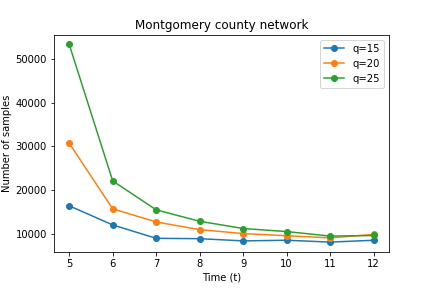
\includegraphics[width=0.3\textwidth]{{figs/montgomery_p0.0435}.png}
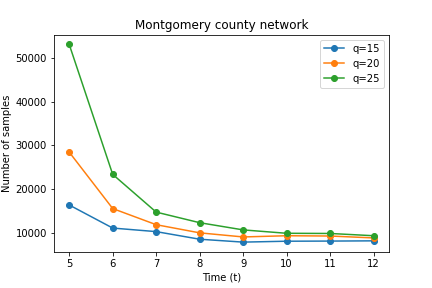
\includegraphics[width=0.3\textwidth]{{figs/montgomery_p0.044}.png}
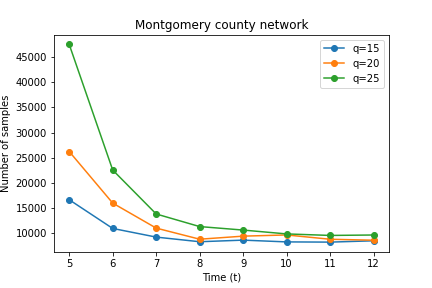
\includegraphics[width=0.3\textwidth]{{figs/montgomery_p0.0445}.png}
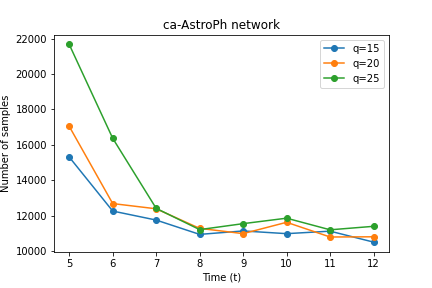
\includegraphics[width=0.3\textwidth]{{figs/ca-AstroPh_p0.0254}.png}
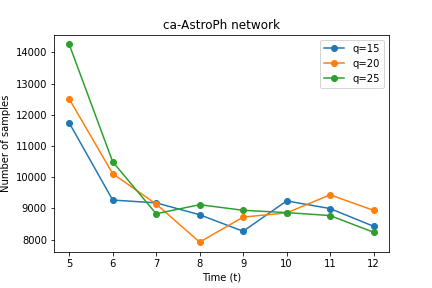
\includegraphics[width=0.3\textwidth]{{figs/ca-AstroPh_p0.03}.png}
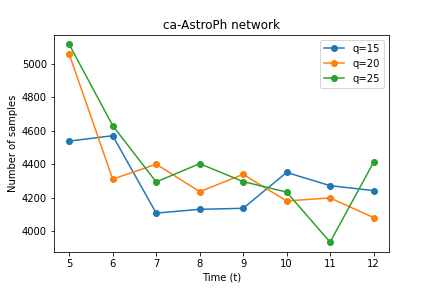
\includegraphics[width=0.3\textwidth]{{figs/ca-AstroPh_p0.06}.png}
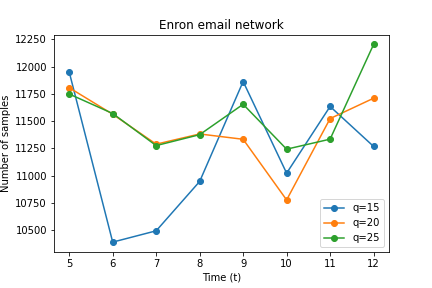
\includegraphics[width=0.3\textwidth]{{figs/email-Enron_p0.0498}.png}
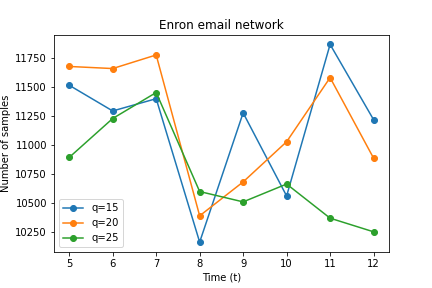
\includegraphics[width=0.3\textwidth]{{figs/email-Enron_p0.0515}.png}
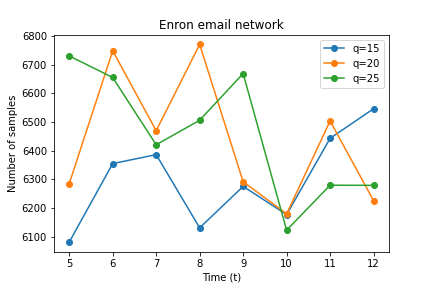
\includegraphics[width=0.3\textwidth]{{figs/email-Enron_p0.098}.png}
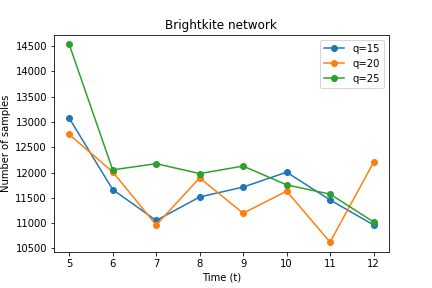
\includegraphics[width=0.3\textwidth]{{figs/loc-brightkite_p0.0693}.png}
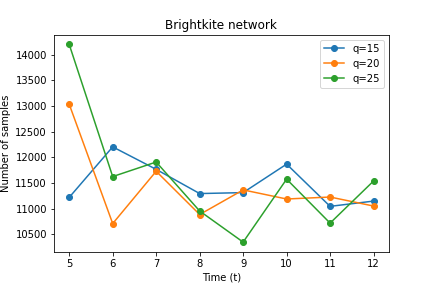
\includegraphics[width=0.3\textwidth]{{figs/loc-brightkite_p0.07045}.png}
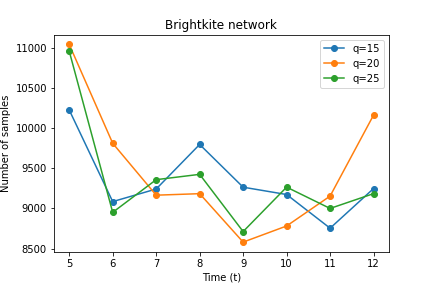
\includegraphics[width=0.3\textwidth]{{figs/loc-brightkite_p0.0852}.png}
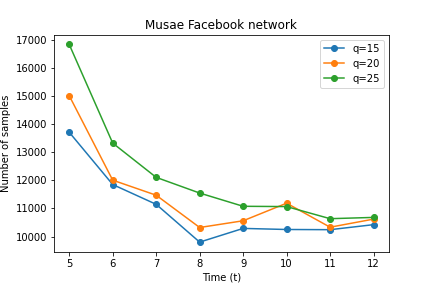
\includegraphics[width=0.3\textwidth]{{figs/musae_facebook_p0.0388}.png}
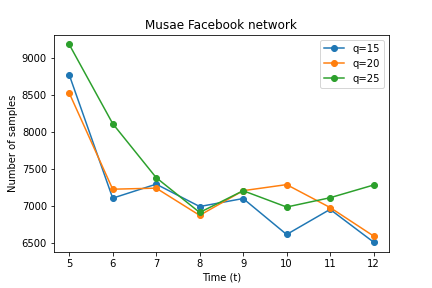
\includegraphics[width=0.3\textwidth]{{figs/musae_facebook_p0.055}.png}
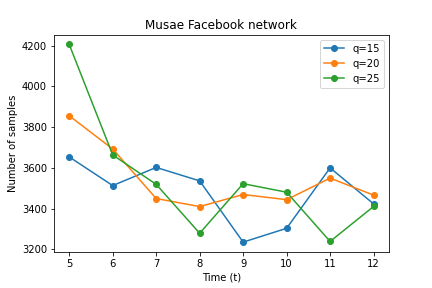
\includegraphics[width=0.3\textwidth]{{figs/musae_facebook_p0.118}.png}
\caption{Number of Monte-Carlo samples using the approach of Dagum et al. \cite{dagum:focs95}
on five different types of networks, as summarized in Table~\ref{tab:datasets}:
a social contact network for Montgomery county, VA, constructed using the approach of
\cite{eubank:nature04, barrett:wsc09} (Row 1),
ca-AstroPh (Row 2), Enron email network (Row 3),
Brightkite location network (Row 4), Facebook network (Row 5).
For each network, we choose three probability values, which ensure that the fraction
of infections is at least 15\% with varying
probability values: low$\sim 0.1$ (left), medium$\sim 0.4$ (middle), and high$\sim 0.7$ (right).
}
\label{fig:dagum-mcmc-montgomery}
\end{figure}

%%%%%%%%% 
\iffalse
\begin{figure}
\centering
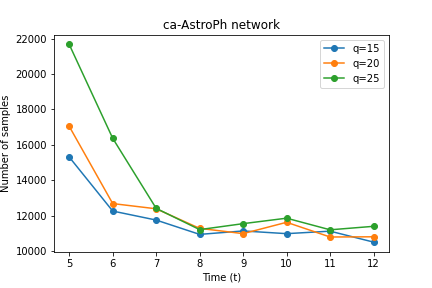
\includegraphics[width=0.3\textwidth]{{figs/ca-AstroPh_p0.0254}.png}
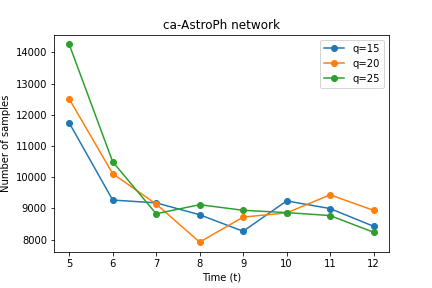
\includegraphics[width=0.3\textwidth]{{figs/ca-AstroPh_p0.03}.png}
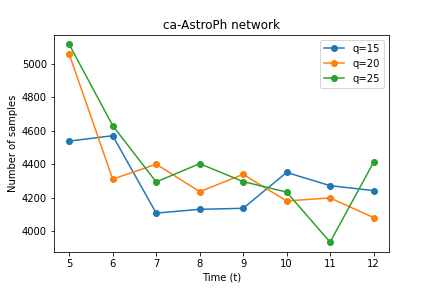
\includegraphics[width=0.3\textwidth]{{figs/ca-AstroPh_p0.06}.png}
\caption{Number of Monte-Carlo samples using the approach of Dagum et al. \cite{dagum:focs95}
for the ca-AstroPh network,
for a transmission probability, such that the expected number of infections 
is around 15\% of the total number of nodes with varying
probability values: low (left), medium (middle), and high (right).
}
\label{fig:dagum-mcmc-ca-astroph}
\end{figure}


\begin{figure}
\centering
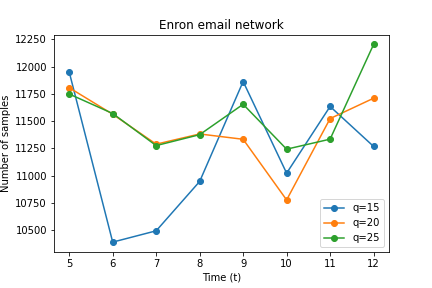
\includegraphics[width=0.3\textwidth]{{figs/email-Enron_p0.0498}.png}
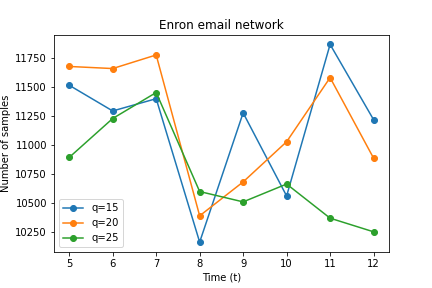
\includegraphics[width=0.3\textwidth]{{figs/email-Enron_p0.0515}.png}
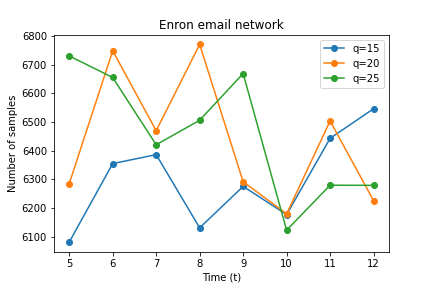
\includegraphics[width=0.3\textwidth]{{figs/email-Enron_p0.098}.png}
\caption{Number of Monte-Carlo samples using the approach of Dagum et al. \cite{dagum:focs95}
for the Enron email network,
for a transmission probability, such that the expected number of infections 
is around 15\% of the total number of nodes with varying
probability values: low (left), medium (middle), and high (right).
}
\label{fig:dagum-mcmc-enron}
\end{figure}


\begin{figure}
\centering
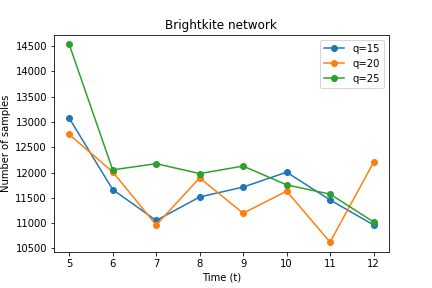
\includegraphics[width=0.3\textwidth]{{figs/loc-brightkite_p0.0693}.png}
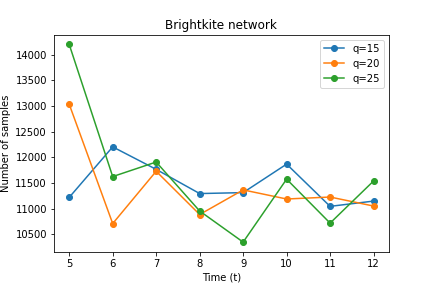
\includegraphics[width=0.3\textwidth]{{figs/loc-brightkite_p0.07045}.png}
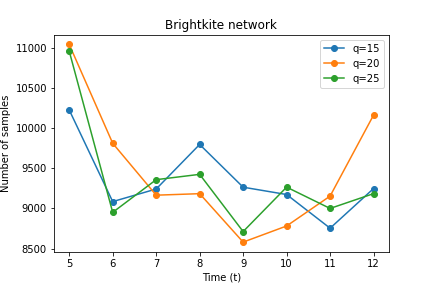
\includegraphics[width=0.3\textwidth]{{figs/loc-brightkite_p0.0852}.png}
\caption{Number of Monte-Carlo samples using the approach of Dagum et al. \cite{dagum:focs95}
for the Brightkite location network,
for a transmission probability, such that the expected number of infections 
is around 15\% of the total number of nodes with varying
probability values: low (left), medium (middle), and high (right).
}
\label{fig:dagum-mcmc-brightkite}
\end{figure}


\begin{figure}
\centering
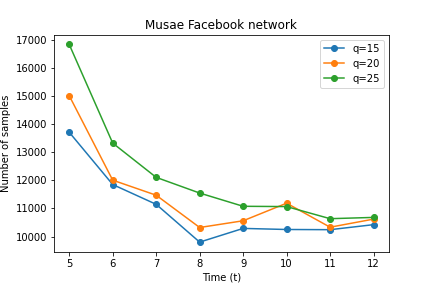
\includegraphics[width=0.3\textwidth]{{figs/musae_facebook_p0.0388}.png}
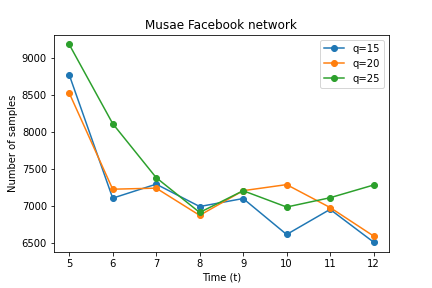
\includegraphics[width=0.3\textwidth]{{figs/musae_facebook_p0.055}.png}
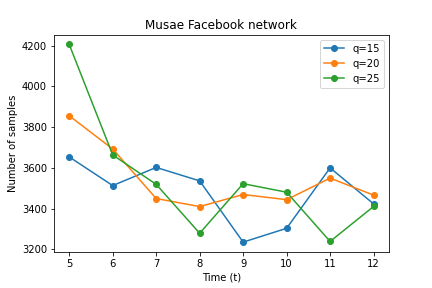
\includegraphics[width=0.3\textwidth]{{figs/musae_facebook_p0.118}.png}
\caption{Number of Monte-Carlo samples using the approach of Dagum et al. \cite{dagum:focs95}
for the Musae Facebook network,
for a transmission probability, such that the expected number of infections 
is around 15\% of the total number of nodes with varying
probability values: low (left), medium (middle), and high (right).
}
\label{fig:dagum-mcmc-facebook}
\end{figure}
\fi



\section{Conclusions and Future Work}
\label{sec:concl}

We formulated several short term forecasting problems under
the SIR model. 
Our results show that many of these problems are computationally
intractable even when the time horizon is as small as two.
These results supplement the reasons discussed in
\cite{Drake-2005,Drake-2006} for the difficulty of accurately predicting
several disease parameters. 
We also presented extensions of our results to realistic 
social networks.
Further, we demonstrated the tightness of our complexity results 
by showing that many of the problems can be solved efficiently
when the time horizon is one.
We also presented randomized approximation algorithms for 
some short term forecasting problems. 
In addition, we showed how our results can be extended to a
number of additional forecasting measures introduced in \cite{TC+2016}
and to three other common epidemic models. 

We close by pointing out some directions for future research.
One direction is to investigate whether there are useful classes
of social networks for which short term forecasting problems can be
solved efficiently. 
In a companion paper \cite{Rosenkrantz_etal_2016}, we have
shown that many forecasting problems under the SIR model can be solved efficiently
when the treewidth of the underlying graph is bounded.
A second direction is to study the complexity of the problem of 
determining the expected number of infections at time $t$, 
where $t$ is a \emph{fixed} value $\geq 3$. 
(We showed in Section~\ref{sec:poly_versions} that the problem can be 
solved efficiently for $t = 1$ and $t = 2$.) 
We also showed that the problem of computing the probability 
of reaching a configuration
that satisfies an $r$-symmetric constraint in one time step
can be solved efficiently.
It is of interest to investigate whether this result can be
extended to other forms of constraints or to special classes of
networks.
Another direction is to study forecasting problems where the input consists
of two or more networks and the goal is to determine which of the networks 
is more likely to cause a given number of infections at a specified time.
Finally, it is also of interest to study forecasting problems
under a model where the initial configuration is specified by a 
vector of probability values, with each value denoting the probability
that the corresponding node is in state \istate{}.
   %% Conclusions, etc.

%%% Bibliography.
\clearpage
\baselineskip=\normalbaselineskip

%%\bibliographystyle{plain}
\bibliographystyle{abbrv}
\bibliography{sir_references.bib,epi-refs.bib}

\clearpage

\baselineskip=1.3\normalbaselineskip
\begin{center}
\Large{\textbf{Appendix}}
\end{center}

\noindent
\textbf{Statement of Theorem~\ref{thm:hardness_for_whole_set}:}~
\begin{description}
\item{(1)}
\emph{
For any $t \geq 2$,~ the problems \tNewInfv,~ \tTotInfv{} ~and \\
\tTotVulv{} ~are~ \cnump-hard.
}

\item{(2)}
\emph{
Unless \textbf{P} = \cnp,
for each of the problems \tNewInfv, \tTotInfv{} and
\tTotVulv{} and for any $t \geq 2$,
there is a constant $\epsilon > 0$
such that if $p^*$ is the actual solution value,
the quantity $\log{(2^n\,p^*)}$ cannot be approximated to within the factor
$O(n^{\epsilon})$ in polynomial time, where $n$
is the maximum number of nodes that can get infected at $t-1$.
}
\end{description}

\medskip

\noindent
\textbf{Proof of Part (1):}~ 

\medskip
\noindent
\textbf{Proof for} \tNewInfv:~ 
We first consider the case where $t = 2$.
The reduction from \mtsat{} for this problem is identical to the one for
\tNewInfs{} for $t = 2$ given in the proof of 
Part~(1) Theorem~\ref{thm:gen_hardness}.
In that reduction, we note that every node that gets infected at $t = 2$
is a member of the node $V_2$ which contains $m$ nodes.
Therefore, the probability that at least $m$ nodes of the entire
node set $V$ get infected at $t = 2$ is equal to the probability that
all the $m$ nodes in $V_2$ get infected at time $t = 2$.
The latter probability is equal to $N/2^n$, where $n$ and $N$ denote 
respectively the number of variables in and the number of satisfying
assignments of the given \mtsat{} instance.
The result for \tNewInfv{} for $t = 2$ follows.
The construction for $t \geq 3$ is also identical to that presented
in the proof of Theorem~\ref{thm:gen_hardness}.  

\medskip
\noindent
\textbf{Proof for} \tTotInfv:~
Again, we first consider the case where $t = 2$.
We modify the construction of graph $G(V,E)$ 
and other components of the problem instance from the construction
used in the proof of Theorem~\ref{thm:gen_hardness} as follows.

\begin{description}
\item{(a)} Node sets $V_0$ and $V_1$ are unchanged.
Node set $V_2$ is modified to contain $mn$ nodes; further, 
$V_2$ is partitioned into $m$ subsets $W_1$, $W_2$, \ldots $W_m$,
where, for $1 \leq j \leq m$, subset $W_j = \{w_j^1, w_j^2, \ldots, w_j^n\}$ 
corresponds to clause $C_j$ and contains $n$ nodes.
Thus, $|V| = mn+n+1$.

\item{(b)} Edge set $E_1$ is unchanged. Edge set $E_2$ is modified as follows.
For each clause $C_j = (x_a \vee x_b)$, $1 \leq j \leq m$,
$E_2$ has the following $2n$ edges: 
$\{v_a, w_j^1\}$, $\{v_a, w_j^2\}$, $\ldots$, $\{v_a, w_j^n\}$, 
$\{v_b, w_j^1\}$, $\{v_b, w_j^2\}$, $\ldots$, $\{v_b, w_j^n\}$.
Thus, $|E| = n+2mn$.

\item{(c)} The value of $q$ in specifying event \cale{} is 
given by $q = mn + 2$.
\end{description}

\noindent
The construction of the transmission probabilities and initial
configuration are unchanged.
The event \cale{} whose probability is to be computed 
is that the number of nodes of $V$ in state \istate{} or 
state \rstate{} at $t = 2$ is at least $mn + 2$.  

To prove that the probability of \cale{} is $N/2^n$,
we establish the following: (i) each infection pattern 
corresponding to a satisfying
assignment for the \mtsat{} instance causes 
all $mn$ nodes in $V_2$
to get infected at time $t = 2$, thereby making event \cale{} occur, 
and (ii) each infection pattern corresponding to a non-satisfying assignment 
causes at most $(m-1)n$  nodes in $V_2$
to get infected at time $t = 2$, 
thereby preventing event \cale{} ~from occurring.
The proof is again in two parts.

\noindent
\underline{Part 2.1:}~
Consider any infection pattern that corresponds to a
satisfying assignment.
Since the assignment satisfies all clauses, at time $t = 2$,
each node in $V_2$ has at least one edge to a node 
in state \istate{} in $V_1$.
Moreover, at least one node in $V_1$ is in state \istate{}  at $t = 1$. 
Thus, including node $s$ which was infected at time 0,
at least $mn+2$ nodes are infected by time $t = 2$.  

\noindent
\underline{Part 2.2:}~
Consider any infection pattern that corresponds to a
non-satisfying assignment.
Then, there is at least one clause $c_j$ that is not satisfied.
Each node in set $W_j$ has two neighbors, say $v_a$ and $v_b$,
in $V_1$, and both $v_a$ and $v_b$ are in state \sstate{} at the 
end of time step $t = 1$.
Therefore, the nodes in $W_j $ cannot be infected at $t = 2$.
Thus, even if every node in $V_1$ gets infected at time $t = 2$,
at most $1 + n + (m-1)n$ nodes are infected by  time $t = 2$,
that is, the total number of nodes infected  by  time $t = 2$ 
is at most $mn+1$.

This completes the proof of \cnump-hardness of \TwoTotInfv.
The \cnump-hardness of\\ \tTotInfv{} for set $V$ for any $t \geq 3$ can be 
proven in a manner similar to that used in the proof of 
Theorem~\ref{thm:gen_hardness}.


\medskip
\noindent
\textbf{Proof for} \tTotVulv:~
Again, we first consider the case where $t = 2$.
We remind the reader that \tTotVulv{} problem at $t = 2$
requires the computation of the probability that \emph{all} the nodes
in $V$ get infected \emph{by} time $t = 2$.
We modify the construction of graph $G(V,E)$ 
and other components of the problem instance from the construction
used in the proof of Theorem~\ref{thm:gen_hardness} as follows.

\begin{description}
\item{(a)} Node sets $V_0$, $V_1$ and $V_2$ are unchanged.
Thus, $|V| = m+n+1$.

\item{(b)} Edge sets $E_1$ and $E_2$ are unchanged. 
An additional set of edges, denoted by $E_3$, includes an edge
between every pair of nodes in $V_1$.
(The edges in $E_3$ ensure that the nodes of $V_1$ form a clique.)
Hence, $|E| = n(n+1)/2+2m$.

\item{(c)} The transmission probabilities of the edges in $E_1 \cup E_2$
remain the same as before.
The transmission probability of each edge in $E_3$ is set to 1.
\end{description}

\noindent
Consider any satisfying assignment for the given \mtsat{} instance.
Such an assignment must infect at least one node in $V_2$ at $t = 1$ and
causes all the nodes in $V_2$ to get infected at $t = 2$.
Since the nodes in $V_1$ form a clique and the transmission probability
of each edge in that clique is 1, any node of $V_1$ which is in state \sstate{}
at $t = 1$ gets infected at $t = 2$.
In other words, every satisfying assignment to the \mtsat{} instance causes
all the nodes in $V$ to be infected \emph{by} time $t = 2$.
Any assignment that does not satisfy the given \mtsat{} instance leaves
at least one node of $V_2$ to remain in state \sstate{} at $t = 2$.
Therefore, the probability that all nodes of $V$ get infected by $t = 2$
is equal to the probability that an assignment chosen uniformly randomly
satisfies the given \mtsat{} instance.
It follows that the \tTotVulv{} problem is \cnump-hard for $t = 2$.
The \cnump-hardness of \tTotVulv{} for any $t \geq 3$ can be 
proven in a manner similar to that used in the proof of 
Theorem~\ref{thm:gen_hardness}.

\medskip

\noindent
\textbf{Proof of Part (2):}~ The reductions used in proof of Part~(1) above show
that for each of the three problems, the solution value $p^*$ is the
probability that the an assignment chosen uniformly randomly from the set
of all possible assignments to the \mtsat{} instance.
Also, in each case, $n$ is the maximum number of nodes that can get
infected at time $t-1$.
Thus, the result of Part~(2) follows using the same argument as the one
used to prove Part~(2) of Theorem~\ref{thm:gen_hardness}.
\QED


\end{document}
